\RequirePackage[l2tabu, orthodox]{nag} %Package complains about uses of old functions, make sure you write modern latex
\documentclass[letterpaper,10pt,twoside]{report}
\usepackage[english,canadian]{babel}
\usepackage{amsmath} %AMS Math Package
\usepackage{amssymb} %AMS Math Symbols
\usepackage[all,warning]{onlyamsmath}%Warn about non-ams math useage, suggest improvements
\usepackage[letterpaper,top=3.8cm,bottom=2.5cm,inner=2.5cm,outer=3.8cm]{geometry} %Sets up basic page dimensions
\usepackage[newcommands]{ragged2e} %provides better \right \left and \Centering, replaces old commands with improved ones
\usepackage[tracking=true,kerning=true,expansion]{microtype} %makes type look better
\usepackage{booktabs} %makes tables look better
\usepackage{siunitx} %provides standard printing for SI units
\usepackage[breaklinks,hidelinks]{hyperref} %Provides clickable links
\usepackage[capitalize,noabbrev]{cleveref} %Allows use of \cref, which knows what kind of ref you're making, so you don't have to write EQN and such
\usepackage{ifpdf} %Conditions for if pdftex is running
\usepackage[T1]{fontenc} %upgrades font encodings
\usepackage[utf8]{inputenc}%Tells latex the file is saved as UTF-8 (make sure it is!)
\usepackage{lmodern} %improved version of computer modern font
\usepackage{multirow} %Allows for mulirow a.k.a. grouped cells in tables
\usepackage{fixltx2e} %Fixings bugs in latex2e that aren't fixed due to breaking backwards compatability
\usepackage{upgreek} %Provides upright (non italic) greek fonts
\usepackage{gensymb} %Provides  \de­gree, \cel­sius, \pert­hou­sand, \mi­cro and \ohm amongst others
\usepackage{textcomp}
\usepackage{textgreek} %Provides \textbeta and similar greek letters in text mode
%\usepackage[section]{placeins} %Fixes placement of figures so they don't cross section boundaries
\usepackage[section,subsection,subsubsection]{extraplaceins} %Modified version of placeins which works at section, subsection and subsubsection
\usepackage{verbatim}%Fixes bugs in \verbatim, and provides \begin{comment} and \verbatiminput for including files
\usepackage{syntonly}%Provides syntax-only latex runs, useful for when the document starts getting big!
\usepackage{csquotes}
\usepackage{float} %Fixes up floats (figures) and provides the H placement modifier (place the float RIGHT HERE). with great power...
\usepackage[style=numeric-comp,backend=biber,sorting=none]{biblatex}
\addbibresource{library.bib}
\addbibresource{nanogold.bib}
\addbibresource{nanocdte.bib}
\addbibresource{srtio3.bib}
\usepackage[english]{isodate}%Convert any date formats to ISO style
\usepackage{listing}%Package for listing sourcecode with syntax highlighting
\usepackage{ellipsis}%Fix \ldots and similar commands, bugs with spacing and such
\usepackage{graphicx}
\usepackage{wasysym}

\pdfminorversion=5
\pdfobjcompresslevel=3 
\pdfcompresslevel=9

\usepackage{subcaption} %The standard method to do figures with a), b) and such
\usepackage{fancyhdr} %Package for changing header/footer
%\usepackage{showkeys} %Prints all instances of \label in margin for easy writing
%\usepackage{lineno} %Allows labeling of line numbers throughout document
\usepackage{makeidx} %For generating index files
\usepackage{lipsum} %Prints junk text with \lipsum
\usepackage{setspace} %Provides \doublespacing command
\usepackage{todonotes} %Provides \todo{something} which puts labels in magin and \missingfigure{something} to put in placeholder figures

\widowpenalty=300 %Prevent widows (single sentences at end of page)
\clubpenalty=300 %Prevent orphans (single sentences on empty pages)
%\doublespacing %Uncomment to turn on double spacing
\onehalfspacing
%\linenumbers %Uncomment to turn on line numbers
%\syntaxonly %Uncomment to only check compile for syntax PRODUCES NO OUTPUT
\hyphenation{nano-wires nano-wire ad-atom wurt-zite nano-structures vi-cinal nano-twins off-cut crys-tal-lites epi-tax-i-ally micro-twinning eq-ui-ang-u-la-tion}

\hypersetup{
    unicode=true,
    pdftoolbar=true,
    pdfmenubar=true,
    pdffitwindow=false,
    pdfstartview={FitH},
    pdftitle={My title},
    pdfauthor={Gabriel A. Devenyi},
    pdfsubject={Subject},
    pdfkeywords={keyword1} {key2} {key3},
    pdfnewwindow=true,
    colorlinks=false,
    linkcolor=red,
    citecolor=green,
    filecolor=magenta,
    urlcolor=cyan
}
\graphicspath{{figures/}} %Uncomment if you want to hide all figure files in a graphics/ subdirectory

\title{The Role of Energy and Symmetry at Epitaxial Interfaces}
\author{Gabriel A. Devenyi}
\date{\today}

\makeindex

\begin{document}

\begin{titlepage} %Half-title page for McMaster Formatting
	\vspace*{\fill}\Centering
	The Role of Energy and Symmetry at Epitaxial Interfaces
	\vspace*{\fill}
\end{titlepage}
% % % % % % % % % % % % % % % % % % % % % % % % % % % % % % % % % % % % % %
\begin{titlepage} %Titlepage
\Centering
\vspace*{\fill} %This makes text vertically centered
{\Large The Role of Energy and Symmetry at Epitaxial Interfaces\\
By\\GABRIEL A.\ DEVENYI, B.\ ENG.\\}
\vfill 
A Thesis Submitted to the School of Graduate Studies in Partial Fulfilment of 
the Requirements for the Degree Doctor of Philosophy
McMaster University
\vfill%This pushes copyright to the bottom
\textcopyright Copyright by Gabriel A.\ Devenyi, May 2013
\end{titlepage}
% % % % % % % % % % % % % % % % % % % % % % % % % % % % % % % % % % % % % %
\pagenumbering{roman}
\setcounter{page}{2} %Descriptive note page
{\Large Descriptive Note\\
DOCTOR OF PHILOSOPHY (2013) McMaster University
(Engineering Physics)
Hamilton, Ontario
TITLE: The Role of Energy and Symmetry at Epitaxial Interfaces\\
AUTHOR: Gabriel A. Devenyi, B.\ Eng. (McMaster University)\\
SUPERVISOR: Professor John S. Preston\\
NUMBER OF PAGES: vii, 212}
% % % % % % % % % % % % % % % % % % % % % % % % % % % % % % % % % % % % % %
	\begin{abstract}
		\thispagestyle{plain}
		\setcounter{page}{3}
			Abstract goes here.
	\end{abstract}
% % % % % % % % % % % % % % % % % % % % % % % % % % % % % % % % % % % % % %
	\setcounter{page}{4}
	\chapter*{Acknowledgements}
	My wife, my dog, my parents, my supervisor.
	\newpage

	\tableofcontents
	\listoffigures
	\listoftables
	\newpage
	\pagenumbering{arabic} %Reset page numbering

%Fix all the header/footer according to McMaster Requirements
	\pagestyle{fancy}
	\fancyhead{}
	\fancyfoot{}
	\fancyhead[RE,LO]{McMaster University -- Engineering Physics}
	\fancyhead[LE,RO]{PhD Thesis -- Gabriel A. Devenyi}
	\fancyfoot[CE,CO]{\thepage}

% % % % % % % % % % % % % % % % % % % % % % % % % % % % % % % % % % % % % %
%Thesis starts here

%For large LaTeX documents, it is best practice to separate the material into smaller files so that it is easier to handle, use \input to insert each file into the overall document

\chapter{Introduction}
Epitaxy has been a dominant technological feature since near the very inception of the semiconductor age.
It has also been intimately entwined with the dominant semiconductor up till the present day, silicon.
Silicon has dominated almost every field of semiconductor research for the better part of 40 years, becoming the most well understood material in the world.
This vast focus on silicon has also greatly influenced the thinking of what were at the time fledgling fields, most notably epitaxy.
\emph{Epi-taxis} or ``above --- in an ordered manner'' is the Greek root of the term epitaxy and as it is originally defined, it has been very narrowly interpreted by most of the research field.
Silicon on silicon epitaxy, or homoepitaxy, has been the dominant type of epitaxy both for research and production, due to its relevance to semiconductor chip manufacturing.
This idea of the `ideal' epitaxy as modelled by silicon homoepitaxy has pervaded the thinking of research into the field, with the material systems being most similar as the result being the most researched, and the most successful.

The material systems most similar to homoeptiaxy (besides other homoepitaxy) are the III-V group semiconductors, specifically the Al/Ga/In-P/As/Sb binary/ternary/quaternary family as in \cref{fig:intro_bandgaps}.
These zincblende semiconductors through the manipulation of exact atomic concentration, can be grown from exactly lattice matched to strongly mismatched. These material systems all have covalent or primarily covalent bonds with strongly preferred atomic sites for the atomic species.
When parameters are optimized, epitaxial growth in such systems is orientationally commensurate with the underlying substrate and dominated by strain effects.
\begin{figure}
    \centering
    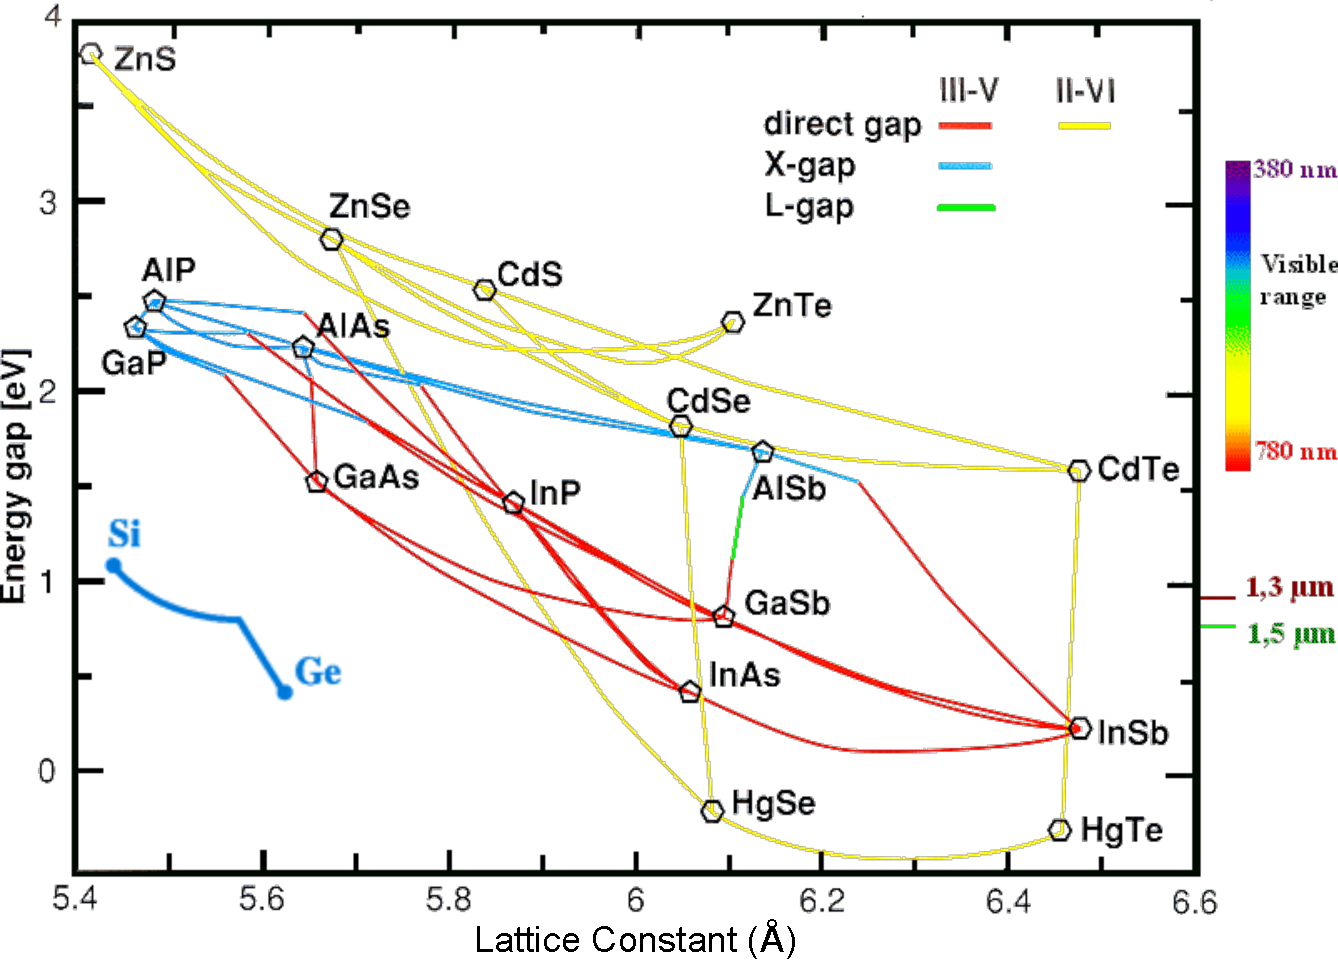
\includegraphics[width=0.9\textwidth]{intro_bandgaps}
    \caption[Bandgap versus lattice constant]{\label{fig:intro_bandgaps}Bandgap versus lattice constant for the most common semiconductors (modified from Helmut\cite{HelmutFoll2013}) (used with permission)}
\end{figure}

Beyond the III-V homologous growth systems, the next most investigated epitaxial process is when these materials are grown on silicon.
In addition to the always-present issue of strain due to the intrinsic lattice mismatch between the III-V family and silicon, the diamond structure of silicon results in an issue of polar (zincblende) on non-polar (diamond) epitaxy\cite{Kroemer1987} where group III and group V atoms cannot differentiate between sites on the silicon surface.
Such site non-specificity has been an issue of great interest to the epitaxy research community resulting in numerous attempts (some successful)\cite{Kroemer1987} to improve growth of such a chemically dissimilar system.

Outside the extensive research into the epitaxy of silicon and the III-V systems, work into epitaxy has mostly been on a material-by-material basis.
Material systems of interest are examined on an issue by issue basis with the goal of producing high quality material for some application, rather than examining the generalized epitaxy phenomenon.
In this work, the goal has been to expand the understanding of epitaxy through an experimental exploration of several model systems which are epitaxial corner cases, and to show other conditions under which high quality epitaxy can occur.
Through this work, two key themes were examined in epitaxial systems, the role of symmetry and the role of energy at epitaxial interfaces.
These themes were examined through investigations into three model material systems, III-V semiconductors on silicon, II-VI semiconductors on crystalline oxides, and noble metals on crystalline oxides.
Investigations into III-V semiconductors on silicon focused on the role of vicinal surfaces, surface reconstructions, and higher order crystal surfaces. Vicinal (or offcut) surfaces of substrates, truncated and reconstructed, were found to have a strong effect on twinning during epitaxial growth, a potential method of improving quality of material growth. (211), a higher order substrate orientation was found to allow accommodation of strain by tilting of a growing epitaxial layer.
Investigations into II-VI semiconductors concentrated on the role of surface reconstructions, and the role of bond strength in epitaxial interfaces. A new epitaxial relationship between temperature stable surface reconstruction and CdTe was observed and atomically modeled, such stable surface reconstructions may offer a new route for lattice matched epitaxial growth. In addition, growths of CdTe on sapphire substrates were found to show a unique liftoff phenomenon, where single crystal films are weakly bonded to the substrate and can be removed while maintaining crystalinity.
Finally, investigations into noble metals on oxide surfaces concentrated on the properties of epitaxy in the weak bonding regime. Epitaxial growth of gold on spinel, a complex oxide, was found to be possible, despite the weak reactivity of both the noble metal and the oxide substrate.
The results from these investigation and the main contribution of this work is to show that epitaxy is possible for symmetrically and chemically dissimilar model systems, and to experimentally examine the implications to epitaxy that such systems have.

\section{Major Themes}
\subsection{Symmetry}
The 2D (and as we shall later see sometimes 3D) interface that separates the epitaxial substrate from the growing crystal has a symmetry relationship which relates the substrate to the crystal.
These surface symmetries are different than the bulk symmetry of the substrate and crystal.
In the simplest treatment of surfaces, the surface of a given substrate is simply a truncation of the crystal in a given orientation, exposing a plane of atoms which then present a subsymmetry of the bulk crystal. Any truncation through a bulk crystal is unstable, since the surface is now exposed to the outside world, and the surface can resolve this instability in a variety of ways.
As will be seen later there are many complications to this model and it is in these complications that we find interesting changes in symmetry, breaks in symmetry and distortions of this 2D surface into a more complex 3D interface.
It is these changes to the surface symmetry, and it's interaction with the growing crystal which have profound and useful implications for epitaxy.
The first major theme investigates the implications of unique interface symmetries, broken symmetries and 3D interfaces on the epitaxial process.

\subsection{Energy}
While symmetry describes the spatial distribution of the landscape presented to a growing crystal, energy describes the magnitude of the effect that landscape has.
Strong energy landscapes cause the symmetry of a given substrate to have it's influence felt strongly, while a weak landscape can have a subtle effect on growth. Whether atoms are bonded via physisorption, covalent bonding, ionic attraction or Van der Walls forces determines the strength of the interface landscape energy.
The energy landscape of the epitaxial interface can vary over a large range, and the role of these strengths has not been examined extensively.
The second major theme of this work investigates the implications of energy landscapes outside the typical heteroepitaxy regime, specifically relating to the weaker energies.

\section{Secondary Themes}
\subsection{Combined Reciprocal Space and Real Space Characterization}
The investigations into epitaxy discussed throughout this thesis have relied upon a variety of techniques to reveal the patterns behind these processes. The most fruitful of the techniques utilized in this work has been the combined use of reciprocal space mapping via 2DXRD and the direct imaging of samples using TEM/STEM. These techniques, when used individually, often lead to ambiguity in the results. STEM/TEM, being a small-area sampling technique can frequently miss information, or cause false interpretations of ``common'' results, when a given sample may be unique or atypical. Similarly, the use of reciprocal space mapping alone gives a picture which convolves all of the data in the sampling area together, providing little insight about its spatial distribution. When these two techniques are combined, the two datasets must be successfully reconciled for a given model of the underlying system to be coherent. Such consistency requirements allow competing explanations to be discriminated from one another based on predictions they make about the data, leading to more complete and less ambiguous models. Such a combination of techniques has also encouraged collaboration, as one cannot be an expert in the operation and interpretation of both systems without compromising the work one originally intended to do.

\chapter{Theory}
\input{theory.tex}
\chapter{Experimental}
\section{Introduction}
The work presented in this thesis, being experimental in nature, hinges on numerous experimental techniques.
The fundamental components of this work rely on extensive use of X-ray diffraction (XRD) and transmission electron microscopy (TEM) in both standard and novel ways.
These techniques will be examined and examined in some detail, as their novel usage is integral to the work presented here.
Several other experimental techniques are also utilized in this work, but they are used in their everyday implementations as seen in the literature.
These experimental techniques will be discussed only briefly for brevity.
The two primary growth techniques used in this work will also be described, however as this work concentrates on epitaxy is a general phenomenon the intricacies and parameter spaces of these techniques will not be considered again for brevity.

\section{X-Ray}
X-rays are high energy photons, generated from the transitions of electrons between their core shell energy levels and bremsstrahlung (the deceleration of electrons).
X-rays have weak interactions with matter, being absorbed or perturbed only slightly upon passing through it.
X-rays have wavelengths comparable with the typical spacings between atoms in crystals, placing them as an ideal non-destructive probe for crystal structure.
X-rays experience elastic scattering when interacting with the electrons surrounding atoms.
The scattering of X-rays, combined with the 3D periodic structure of atoms, results in constructive and destructive interference and X-ray diffraction\cite{zavalij}.
\begin{equation}
 \label{eqn:bragg}
 2d \sin(\theta) = n \lambda
\end{equation}
X-ray diffraction is fundamentally an interference phenomenon, for a set of planes within a crystal separated by some distance (\textbf{d}), they will diffract from those planes at an angle (\textbf{\straighttheta}) depending upon the wavelength (\textbf{\textlambda{}}), this is known as Bragg's law as in \cref{eqn:bragg}.
Bragg's law is identical to the phenomenon of thin film interference of visible light, only differing by the scale.
Bragg's law, while correct, is a one dimensional expression, in three dimensions it can be represented by the Laue equations as in \cref{eqn:lauea,eqn:laueb,eqn:lauec}.
The vectors \textbf{k\textsubscript{i}} and \textbf{k\textsubscript{0}} are the incident and outgoing X-ray beam, \((a,b,c)\) are the primitive vectors of the crystal lattice and \((h,k,l)\) are the reciprocal lattice indices.
Thus, for a given crystal with a fixed unit cell, there are only certain relationships between the incident and outgoing X-ray beams that satisfy the diffraction conditions, resulting in diffraction.
\begin{align}
 a \cdot (k_0 - k_i) = 2 \pi h \label{eqn:lauea} \\
 b \cdot (k_0 - k_i) = 2 \pi k \label{eqn:laueb} \\
 c \cdot (k_0 - k_i) = 2 \pi l \label{eqn:lauec}
\end{align}

A concept known as reciprocal, or momentum space, is a common construct used in solid state physics to discuss the properties of crystals and is intimately related to diffraction.
Reciprocal space can be visualized as a lattice of points, each representing a spacing present in the crystal, and the lattice having the same symmetry as the real crystal.
Reciprocal space is also the Fourier partner of the real space lattice of the crystal.
Reciprocal space provides an opportunity for an alternate expression of the conditions for diffraction, known as the Ewald construction.
The Ewald construction or Ewald sphere expresses the diffraction condition through the overlay of a sphere of radius 1/\textlambda{} pinned on its radius at the origin in reciprocal space, an incident X-ray beam (\textbf{k\textsubscript{i}}) entering the sphere.
The direction of the exiting diffraction beam is determined by the intersection of the surface of the sphere with the reciprocal lattice, as shown in \cref{fig:exp_xray_ewald}.
As a crystal is rotated (or the incoming beam is moved), the Ewald sphere will rotate about the reciprocal space origin, sweeping through reciprocal space and exciting diffraction conditions as the sphere coincides with lattice points.
The pinned rotation of the Ewald sphere about the origin means that only reciprocal lattice points with a radius from the origin of less than 2/\textlambda{} can be excited into diffraction, indicating the effective limitation of a given X-ray source, as well as why light is an ineffective diffraction probe.
\begin{figure}
 \centering 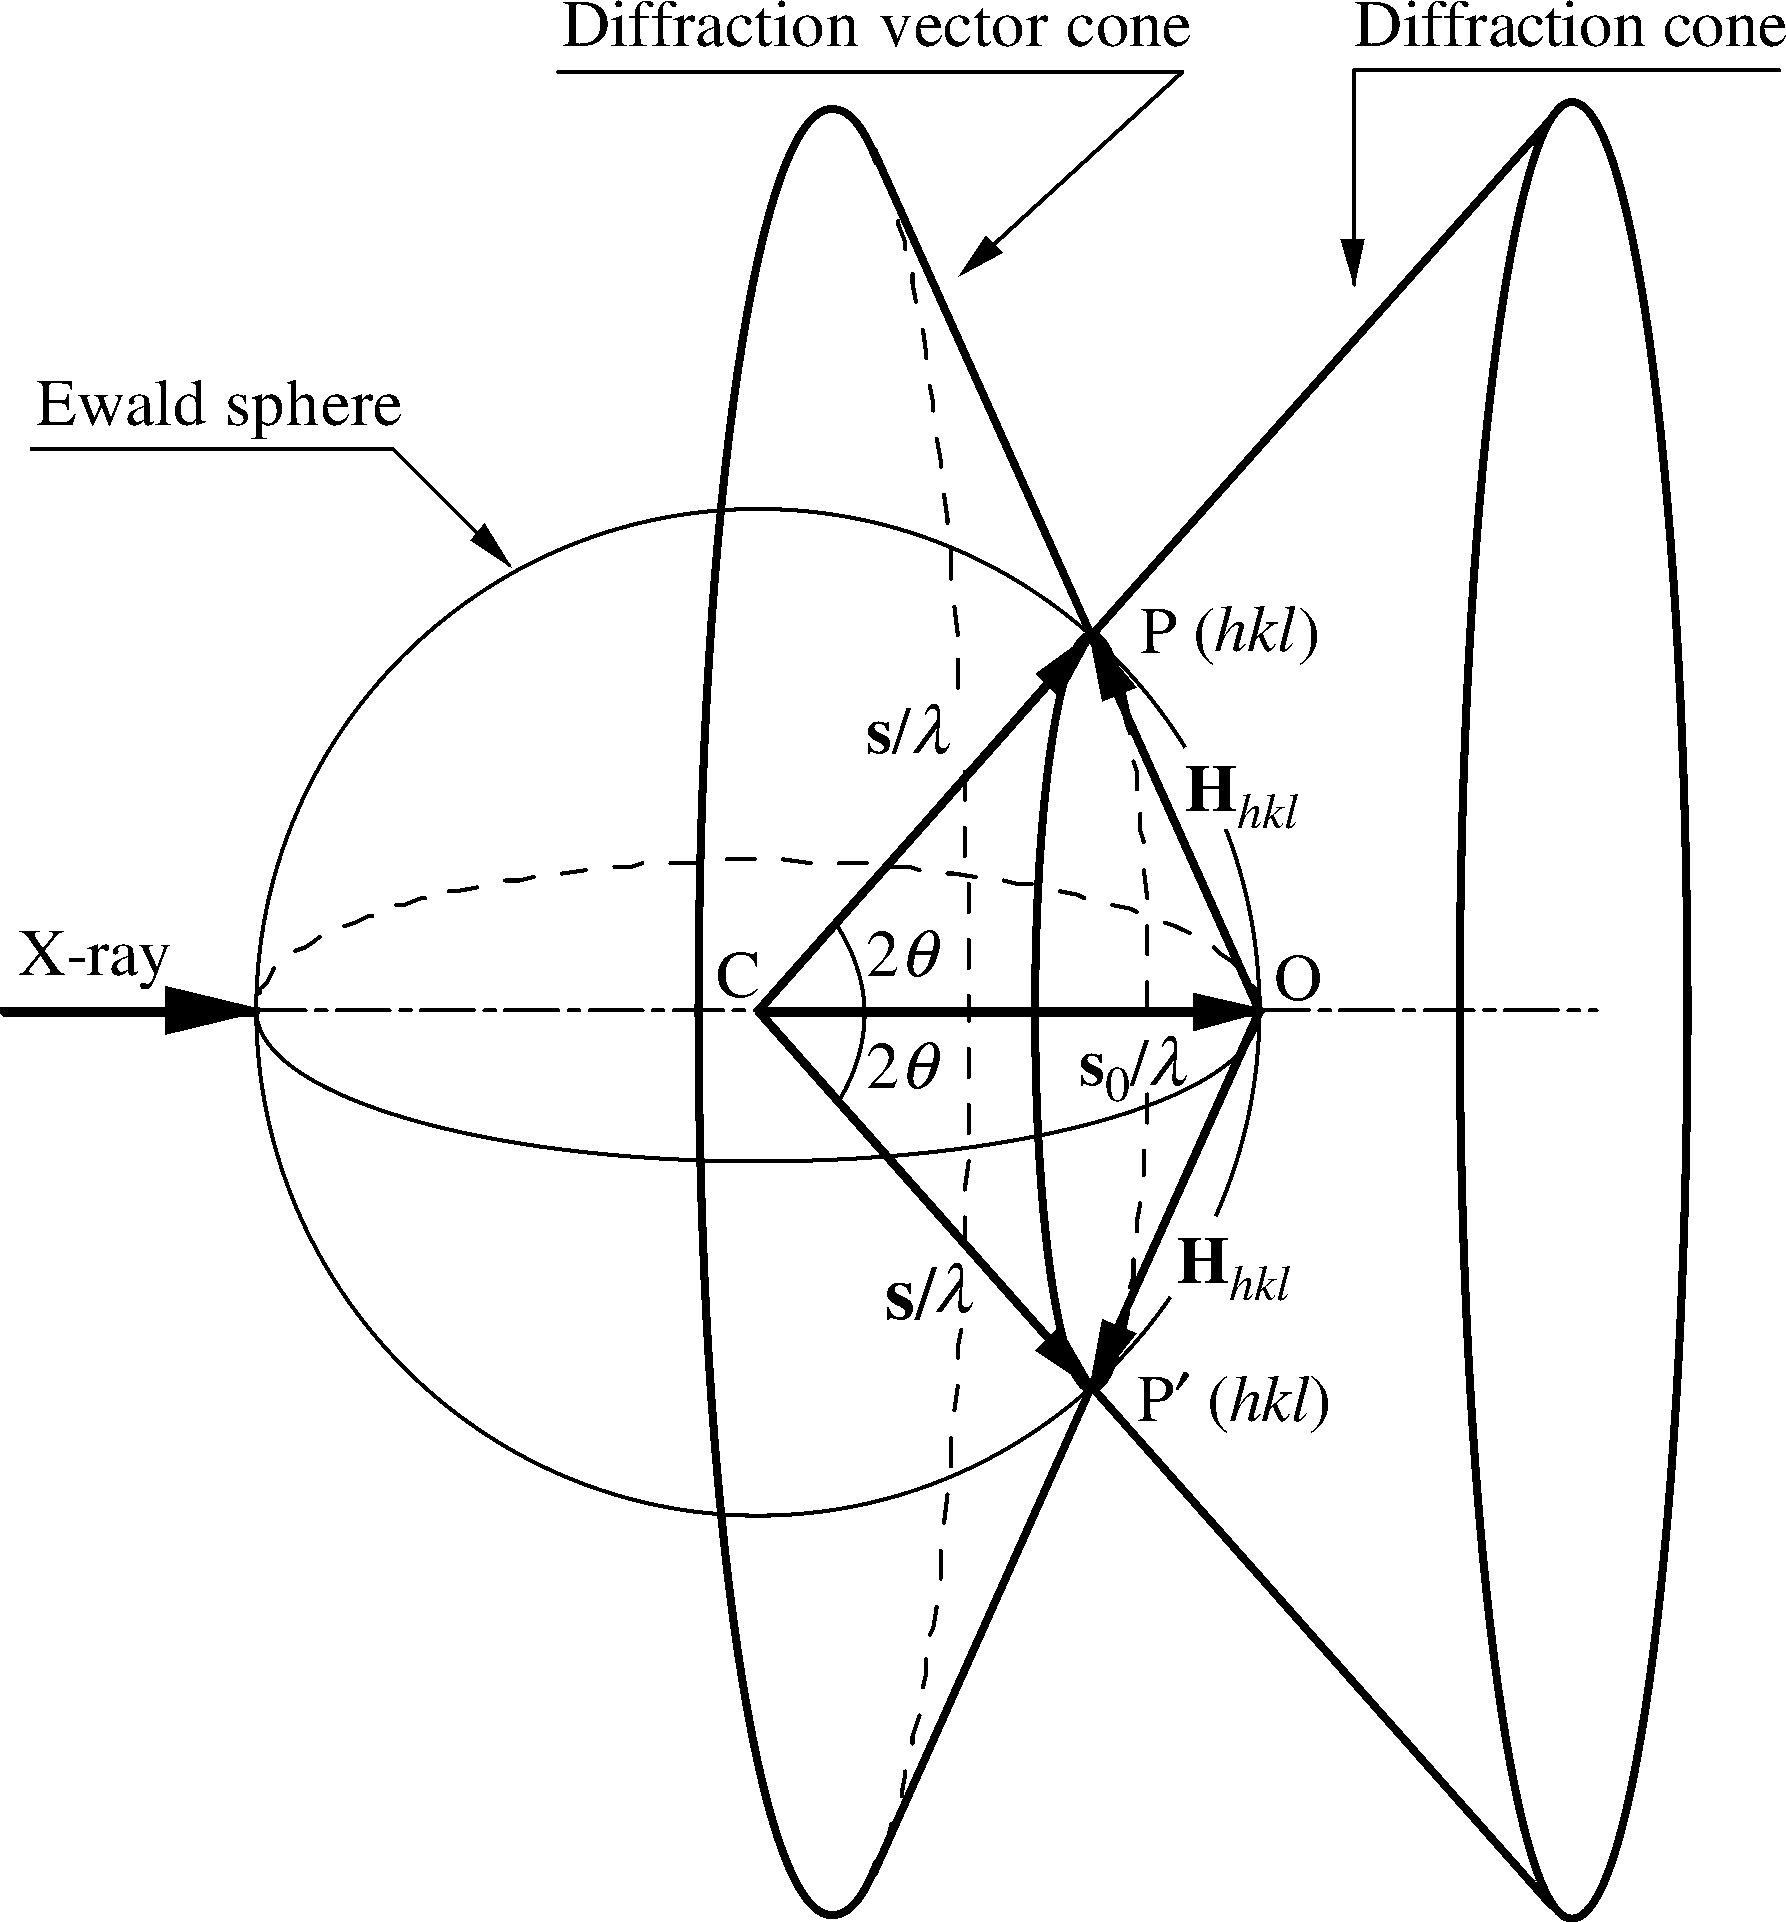
\includegraphics[width=0.6\textwidth]{exp_xray_ewald}
 \caption[Ewald sphere]{\label{fig:exp_xray_ewald}Ewald sphere construction of diffraction conditions (vector form of laue equation) showing incoming X-ray beam to crystal (C) and the reflected and transmitted diffraction cones for a fixed (hkl) and 2\straighttheta{} (used with permission from \cite{He2009})}
\end{figure}

\subsection{2DXRD --- Reciprocal Space Mapping}
\label{sec:2DXRD}
As shown by \cref{eqn:lauea,eqn:laueb,eqn:lauec} and \cref{fig:exp_xray_ewald}, there are a large number of orientations of a crystal which generate diffraction.
For the analysis of crystals, the lowest orders of crystal diffraction (small h,k,l) are the strongest, and provide the least ambiguous information, the they are also at the lowest 2\straighttheta{} values.
This still leaves a significant number of diffraction beams of interest to measure and provide structural information.
The naive measurement technique for collecting this information involves taking a crystal and orienting an incoming X-ray beam, and a detector in configurations that satisfy \cref{eqn:lauea,eqn:laueb,eqn:lauec}.
Such measurements assume that the experimenter knows the orientation and unit cell of the crystal to a degree well enough calculate those configurations.
If either of those pieces of information is unknown, the experimenter must instead sample the 4\textpi{} solid angle (usually only the upper 2\textpi{} half) of angular space surrounding a crystal with enough resolution to intersect with the diffraction conditions of interest.
Such experiments, when performed using a typical X-ray point detector, take inordinate amonts of time, as the angular space is large and the point detector must count for a long time to achieve good counting statistics.

An alternate implementation of such a measurement process is with a 2D planar detector rather than a point detector.
A 2D X-ray detector can subtend a large section the angular space surrounding a given experiment, potentially collecting information about a large section of reciprocal space with each frame it collects.
If configuration is then swept through a range of diffraction conditions, the 2D detector will collect information about a wide swath of reciprocal space.
2DXRD techniques simultaneously collect information about the phase and symmetry of an unknown sample allowing that information to be then examined via a variety of techniques.

\subsubsection{Practical 2DXRD Measurement}
\begin{figure}
 \centering 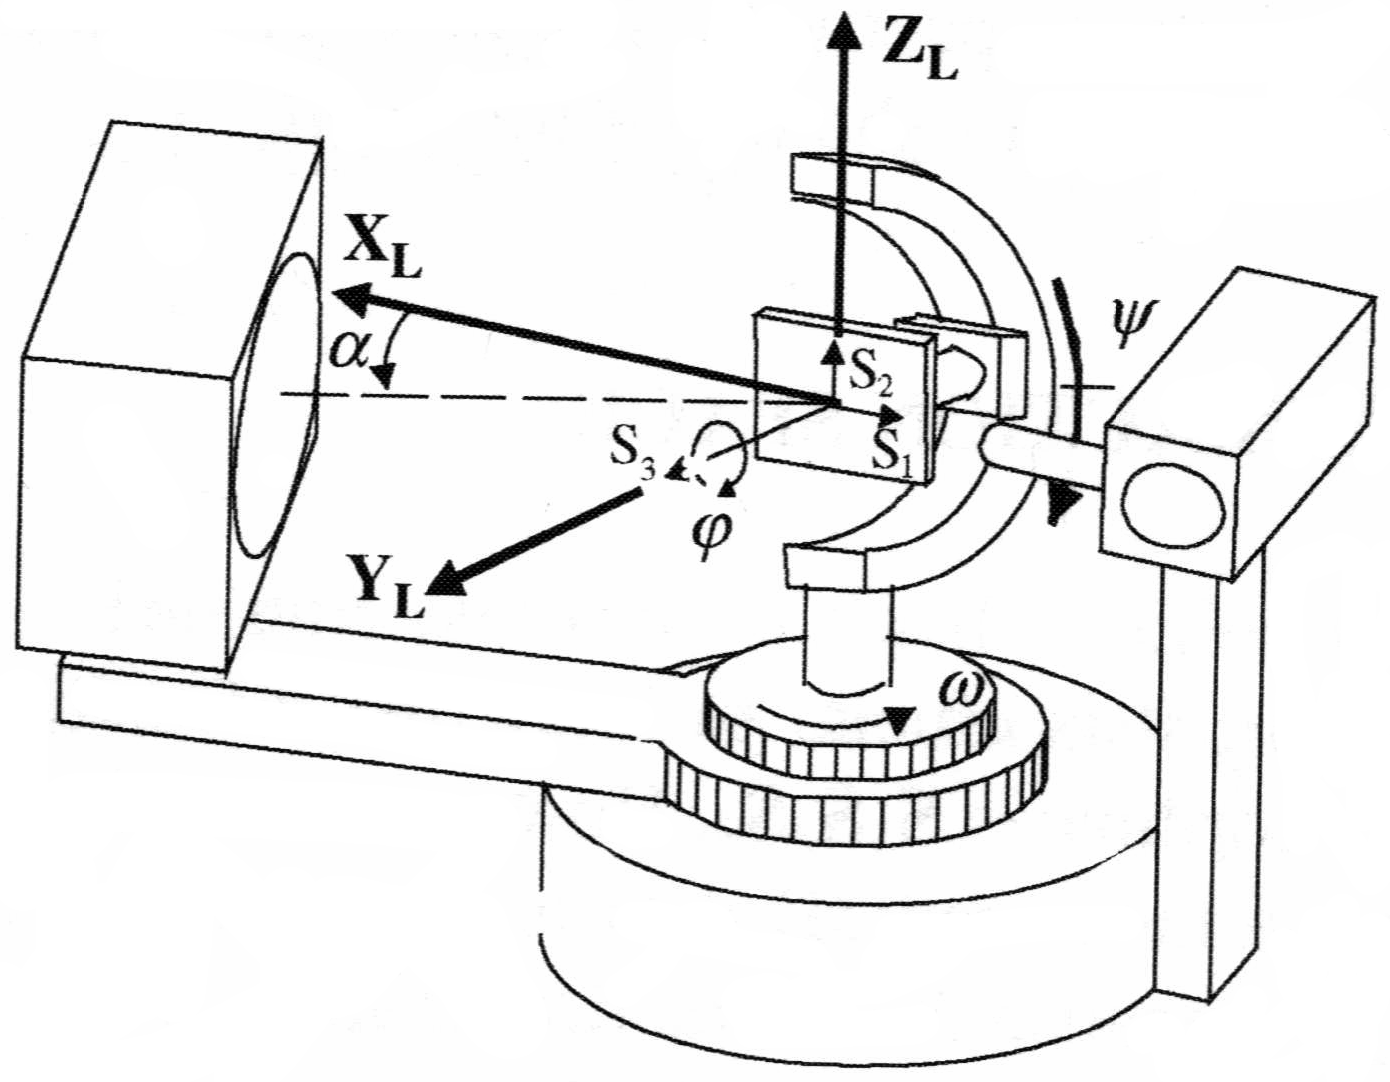
\includegraphics[width=0.8\textwidth]{exp_xray_machine}
 \caption[Typical 2DXRD experimental implementation]{\label{fig:exp_xray_machine}Standard configuration of a 2DXRD system with source, sample and detector, with the sample (S) and laboratory (L) coordinate systems labelled. Standard goiniometer angles are also labelled (used with permission from \cite{He2009})}
\end{figure}
Practical 2DXRD measurements are achieved through the use of a multi-axis goiniometer, a device which maintains the sample at a central point while rotating its orientation relative to the X-ray source and detector.
For epitaxial crystals grown on crystalline substrates, a sample under measurement is placed in the goinometer with its surface normal oriented along the goiniometer's sample axis and a reference edge.
An X-ray source is placed on one arm of the goiniometer and the 2D detector is placed on the other arm.

A standard 2DXRD measurement is performed by configuring the goiniometer (\cref{fig:exp_xray_machine}) such that the X-ray source to 2D detector angle corresponds to a known or presumed low-order 2\straighttheta{} angle for the sample.
The sample was then rotated such that incident angle relative to the surface is shallow, less than 5\degree{}.
Such a beam configuration is ideal for collection of maximum diffraction information, however it can greatly increase the X-ray beam width, as shown in \cref{fig:exp_xray_beam_width} and \cref{eqn:exp_xray_beam_width}.
If the sample of limited size, alternate measurement schemes must be computed.
The sample is then rotated about its surface normal while the 2D detector takes sequential images, a process known as a \textphi{}-scan.
By aligning the sample along 2\straighttheta{} in one dimension, as the sample rotates in a complimentary dimension crystallographic directions that contain the d-spacing corresponding to a range of 2\straighttheta{} around the selected value will be collected on the detector.
The number of frames exposed during this rotation determines the resolution along the rotation direction in reciprocal space, while the resolution of the 2DXRD detector determines the complimentary dimension.
An additional scan of the sample while maintaining the 2\straighttheta{} configuration and scanning the X-ray beam incident angle is known as an \textomega{}-scan.
While the combination of these two scans collects only the reflections surrounding the centred 2\straighttheta{} of interest, if the measurement scheme successfully collects all or the most of the reflections, the symmetry of the underlying system will allow any other reflections to be inferred, greatly reducing overall measurement time.
\begin{figure}
 \centering 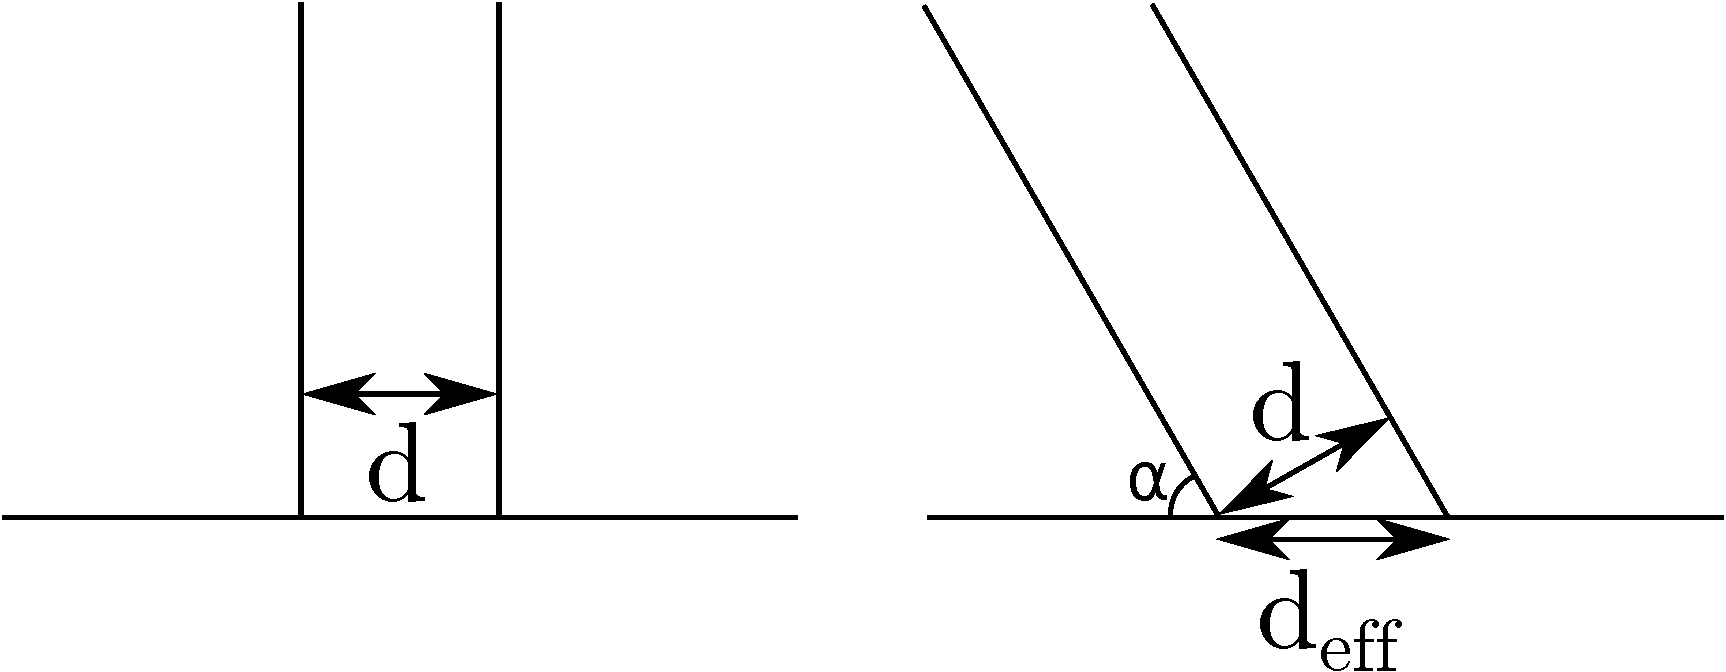
\includegraphics{exp_xrd_beam_width}
 \caption[X-Ray Beam Width]{\label{fig:exp_xray_beam_width}Comparison of beam width and effective beam width caused by inclination of sample}
\end{figure}
\begin{equation}
 d_{eff} = \frac{d}{\sin{\alpha}} \label{eqn:exp_xray_beam_width}
\end{equation}

As reciprocal space mapping is a process which operates in angular space, the distance the detector is an important optimization parameter for 2DXRD measurements.
The distance the 2DXRD detector is situated away from sample will change the solid angle subtended by the detector.
Close detector distances allow the collection of more reciprocal space data in a given scan, at the expense of reducing the resolution due to finite pixel size, as well as increasing the risk of overlap for features close in 2\straighttheta{}.
For epitaxial thing films grown on lattice mismatched substrates, close detector distances can result in substrate and epitaxial crystal peaks overlapping, making interpretation difficult.

The last optimization parameter for 2DXRD scans is the time duration collecting each frame.
For a given brightness of X-ray source and thickness of material, the frame exposure times are ideally set to capture counts just below the maximum the electronics can achieve.
Maximizing the counts for the X-ray detector ensures optimum signal to noise for a given measurement.

\subsubsection{Interpretation of 2DXRD Measurements} Once a 2DXRD measurement has been taken, the resulting data consists of a series of 2D detector frames.
The exact number of frames is determined by the sampling resolution set during the 2DXRD scans.
Each frame is a snapshot of the diffraction intensity collected from the sample for the exact angular configuration in space stored with the frame.
A single 2DXRD frame (\cref{fig:exp_xray_frame}) which contains a X-ray diffraction peak can be analyzed via a number of integration techniques.
The two perpendicular pixel directions on the 2DXRD frames are transformed into two angular dimensions in the coordinate system of the sample, 2\straighttheta{} and \textchi{} \cite{He2009}.
The resulting frame is sliced into hyperbola with the x-direction of the frame corresponding to the radius and a new dimension \textchi{} corresponding to the direction along a given hyperbola.
\begin{figure}
 \centering 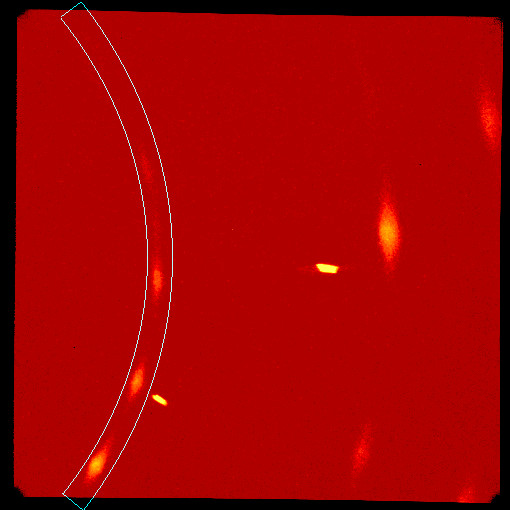
\includegraphics{exp_xray_frame}
 \caption[Example 2DXRD frame]{\label{fig:exp_xray_frame}An example X-ray frame with a conic section of fixed 2\straighttheta{} highlighted}
\end{figure}

The data on a frame can be integrated in one dimensional plots along either dimension of the hyperbola.
Integration of the data along \textchi{} and plotting with respect to 2\straighttheta{} results in a pseudo-powder pattern similar to those taken in a common Bragg-Brantano XRD system, expect it can be performed for diffraction peaks other than perpendicular to the substrate.
Such plots show the presence of d-spacings within the frame of interest, and their width.
Integration of data over a 2\straighttheta{} range and producing a one dimensional plot will show the spatial intensity distribution of a given diffraction peak.
An example 2DXRD frame, with labels of the two diffraction dimensions is shown in \cref{fig:exp_xray_frame}.

\subsubsection{Pole Figure Generation} While integration of the diffraction data on a single frame provides useful quantitative measures of the distribution of a diffraction peak in space, when many frames are collected the generation and interpretation of many frames is tedious difficult to interpret.
Pole figure generation from a set of frames is a method of graphically representing the spatial extent of the diffraction intensity of a given d-spacing around a given sample.
Pole figures readily allow the interpretation of diffraction data to assess crystalinity, presence of phases and orientation relationships between a substrate an epitaxial crystal.
%\begin{figure}
%    \centering
%    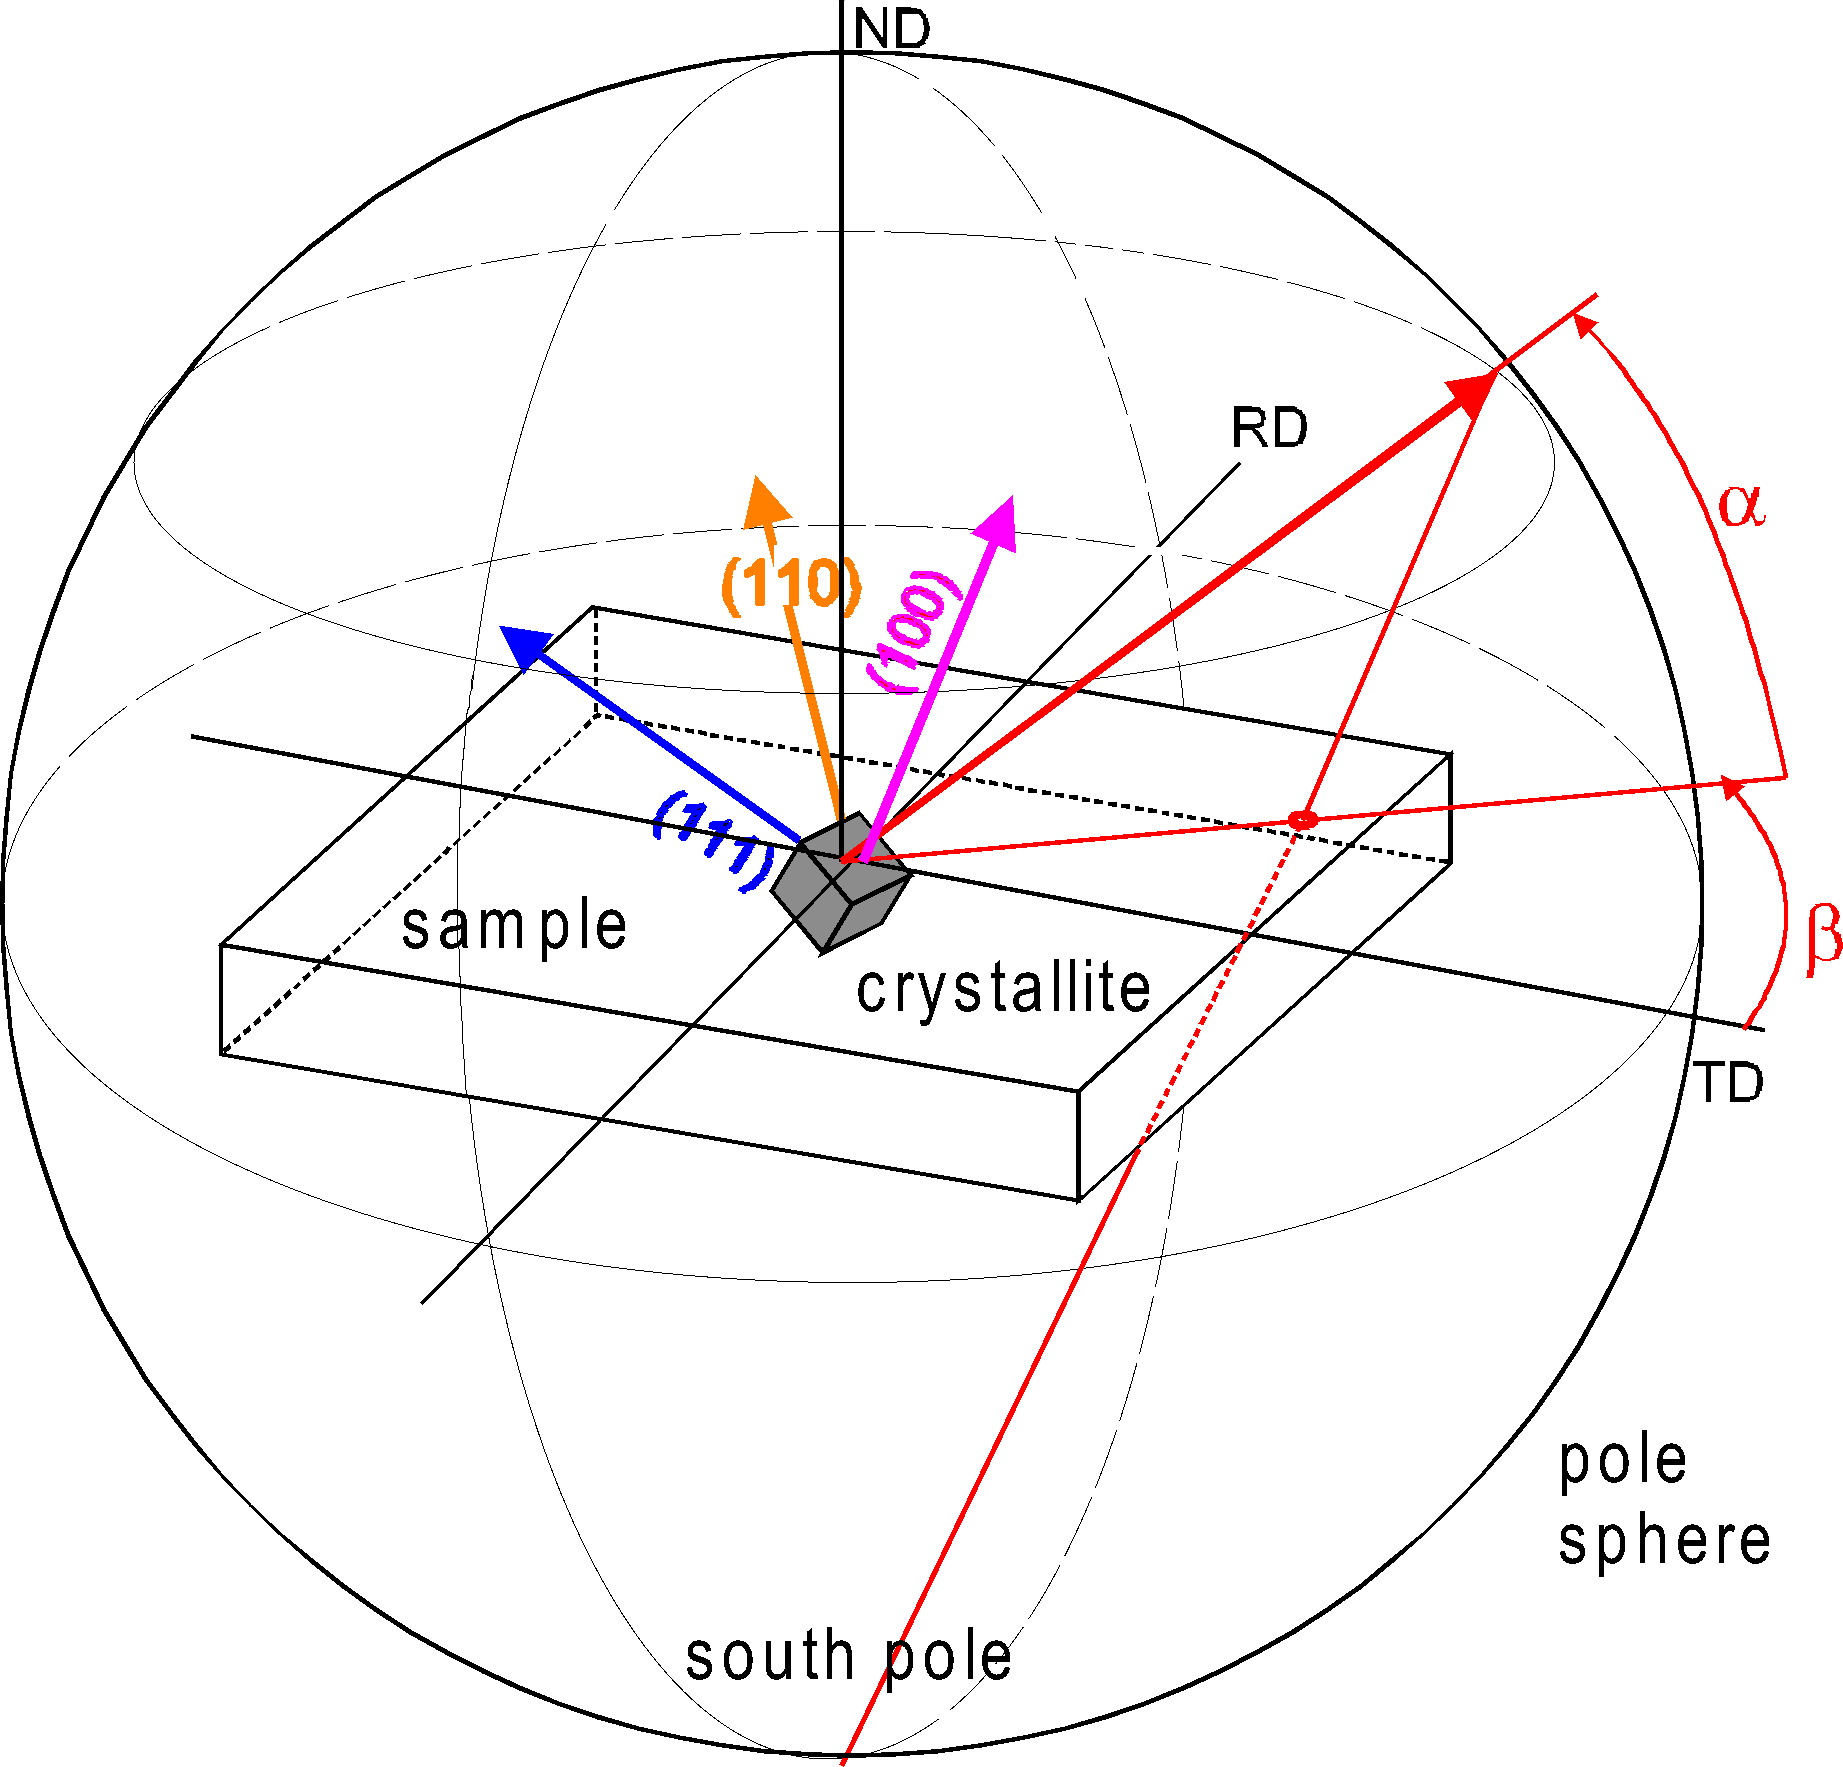
\includegraphics[width=0.7\textwidth]{exp_xray_polesphere}
%    \caption[Mapping of a unit cell to pole sphere]{\label{fig:exp_xray_polesphere}The pole sphere showing the origin of peaks in a pole figure and their relationship to the sample and an individual unit cell\cite{gadds_manual}}
%\end{figure}

To generate a pole figure from a collection of frames a 2\straighttheta{} and \textchi{} range are selected on the first frame of a series of frames.
Generally, such a range will include the maximum width of a single d-spacing of interest (such as \{111\}) and the entire extent of \textchi{} on the frame.
The range is integrated across 2\straighttheta{}, producing a one dimensional intensity scan.
The intensity scan from each frame is then mapped onto the pole sphere (\cref{fig:exp_xray_polefigure}) according to the frame orientation information, forming a geodesic line of intensity.
The pole sphere is a construction centred on the sample which maps the direction in space that diffraction intensity is collected by the detector.
As each frame is integrated, the surface of the pole sphere is painted with colour mapped intensity data.
The resulting sphere of data is then stereographically (angle preserving) projected onto a circle, resulting in a pole figure\cite{He2009}.
The pole figure is a polar diffraction intensity colour map with the radial direction represented by \textalpha{}, the angle from the top of the sphere and the azimutual direction \textphi{} is the in-plane orientation relative to the sample's \textphi{} zero orientation set during sample mounting.
An example pole figure mapping a single data point from the pole sphere is shown in \cref{fig:exp_xray_polefigure}.
\begin{figure}
 \centering 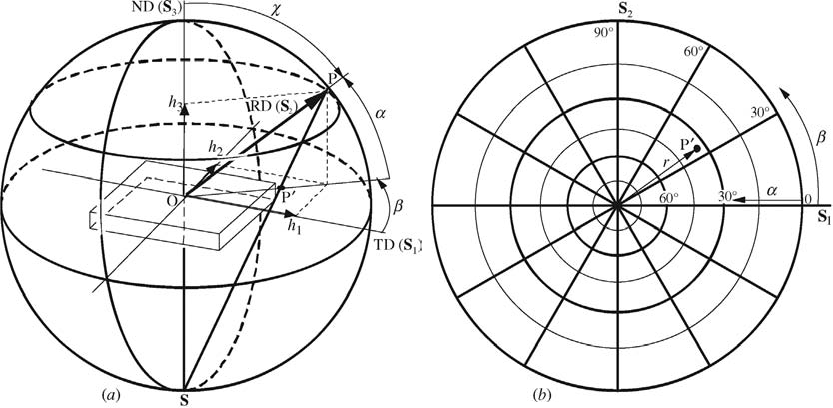
\includegraphics[width=\textwidth]{exp_xray_polefigure}
 \caption[Mapping of pole sphere to pole figure]{\label{fig:exp_xray_polefigure}Example mapping of pole sphere data points to pole figure\cite{He2009}(used with permission)}
\end{figure}

\subsubsection{Interpretation and Simulation of Pole Figures} Once a pole figure has been generated the resulting graphical representation of the diffraction data must be interpreted in the context of the sample composition.
Generally, a pole figure will be generated for a low-index reflection (100,110,111) for both the epitaxial crystal and the substrate.
By generating two figures, the orientation relationship between the diffraction intensity produced by the grown crystal and the single crystal substrate can be examined by comparing the two figures.
\begin{figure}
 \centering \centering
 \begin{subfigure}[t]{0.55\textwidth}
  \centering 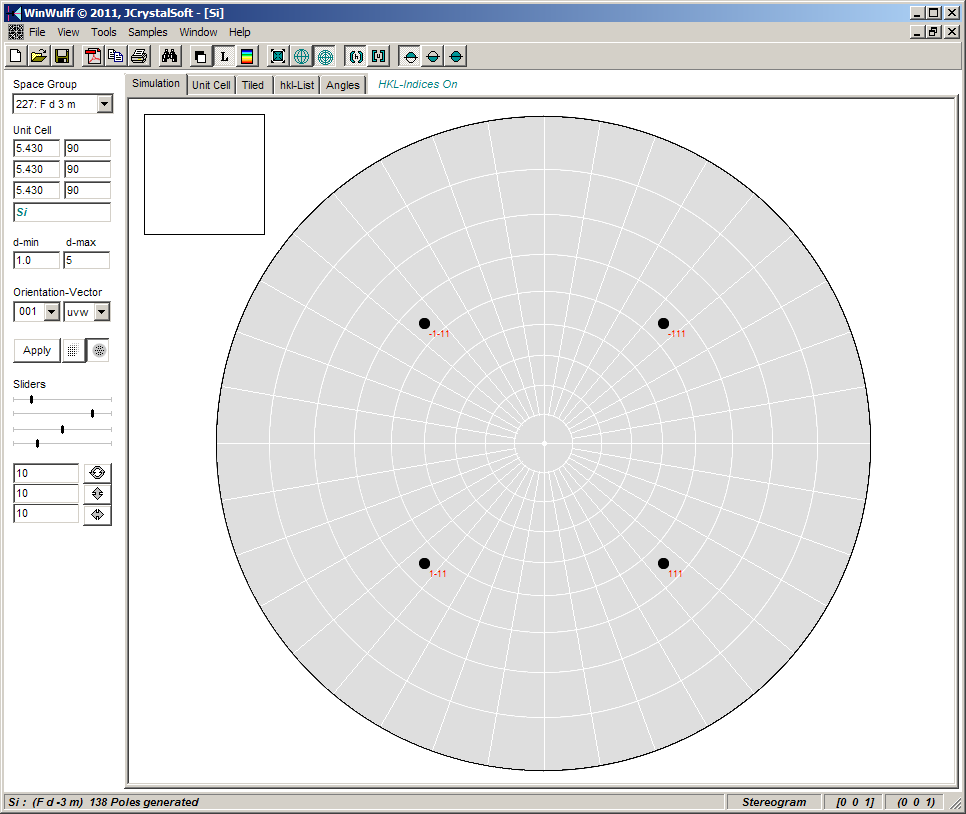
\includegraphics[width=\textwidth]{exp_xrd_winwulff_si_100}
  \caption{\label{fig:exp_xrd_winwulff_si_100}WinWulff (111) pole figure of (100)-up silicon}
 \end{subfigure}%
 \begin{subfigure}[t]{0.45\textwidth}
  \centering 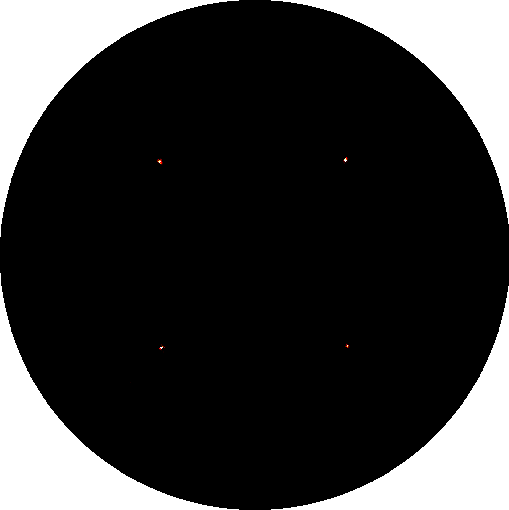
\includegraphics[width=\textwidth]{exp_xrd_si_100}
  \caption{\label{fig:exp_xrd_si_100}Experimentally generated (111) pole figure of (100)-up silicon}
 \end{subfigure}
 \caption{\label{fig:exp_xray_winwulff}Comparison of WinWulff simulation and experimental single crystal silicon pole figure}
\end{figure}

The first step for pole figure analysis is to examine the pole figure generated from the substrate low index reflection.
Since the substrate should be a single crystal, it is trivial to interpret it for its orientation information.
A single crystal pole figure of the substrate can be simulated by considering the space group (cubic, hexagonal, etc.), unit cell, and physical orientation (100-up, 111-up), calculating the surface normals of the d-spacing of interest, collecting them on a pole sphere and mapping them onto a pole figure.
This is conceptually identical to the generation of a pole figure from raw data, except the data is computed from a perfect crystal unit cell.
Such pole figures are simulated using a piece of software such as WinWulff\cite{Weber2006} as seen in \cref{fig:exp_xray_winwulff}, allowing interaction with the pole figure.
The pole figure generated from the data is then compared to the simulated pole figure and the simulation is manipulated by changing the orientation of the crystal until the two figures coincide.
The orientation information provided by the simulation software is now the same as the orientation of the measured crystal.
Such comparison provides the absolute orientation of the crystal in the diffractometer, and all other pole figures generated form the dataset can be referenced to that crystal.

Now that the substrate orientation is known, the pole figure generated from the data can be referenced to the substrate.
If the epitaxial crystal is also a single crystal, the same trivial comparison process can be performed.
The resulting orientation of the eptitaxial crystal can be compared to the substrate, providing the epitaxial relationship.

For the case of systems which have non-ideal epitaxial growth, the pole figures likely contain diffraction intensity information from a number of crystalline sources.
This pole figure as the convolution of the pole figures for each of the components of the epitaxial crystal.
There are several features which arise in such pole figures which are characteristic of certain growth relationships.
A pole figure that, when generated, is uniform in intensity, or has intensity present everywhere with a broad distribution is characteristic of a strongly polycrystalline growth random in orientation, with no epitaxial relationship to the substrate, a simulated pole figure of such a situation is shown in \cref{fig:exp_xray_polefigure_examples}a.
Pole figures which contain bands of diffraction intensity which are rotationally symmetric about their centre are characteristic of a crystal that has a preferred stacking order in the vertical direction, but has no in-plane orientation, such an example is shown in \cref{fig:exp_xray_polefigure_examples}b.
Such preferred stacking orders, usually (111)-up is a common occurrence when growing binary cubic materials.

The most difficult situation that occurs is when the generated pole figure contains multiple single crystal-like peaks.
The presence of single crystal-like peaks indicates a number of different orientations of the epitaxial crystal.
These epitaxial crystals are referred to as textured materials, an example of which is shown in \cref{fig:exp_xray_polefigure_examples}c.
For textured epitaxial crystals, there are number of possibilities for the cause of texturing during growth.
Faced centered cubic binary semiconductors have a propensity to have stacking faults or twins during growth.
The twinned crystallite will create new diffraction peaks in the pole figure, they will have a twin relationship with the host crystal about the twin direction (usually \{111\}).
Other textured epitaxial crystals may arise through multiple preferred growth relationships with the underlying substrate.
Such systems typically have pole figures where the symmetry of the overall pole figure reflects the substrate surface symmetry.
The example in \cref{fig:exp_xray_polefigure_examples}c is one of a (111)-up crystal (3-fold symmetry) on a (100) substrate (4-fold symmetry), showing \(3\times 4=12\) peaks.
\begin{figure}
 \centering 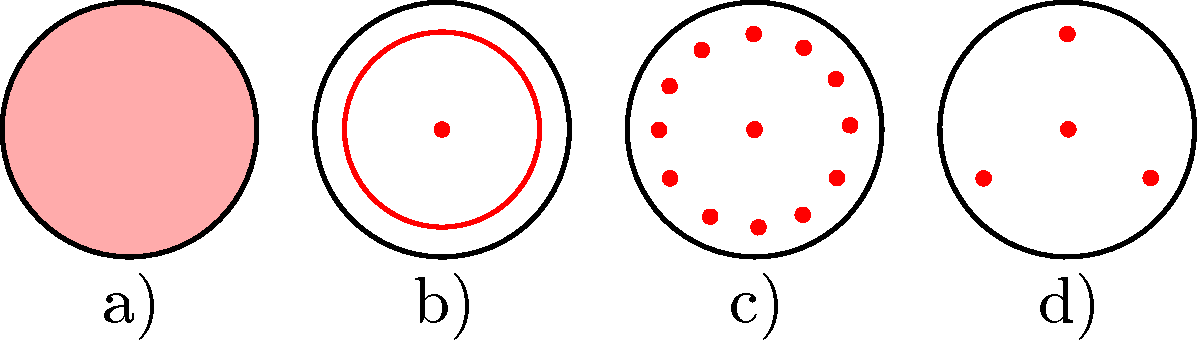
\includegraphics{exp_xray_polefigure_examples}
 \caption[Example simulated pole figures]{\label{fig:exp_xray_polefigure_examples}Example pole figures of a) Polycrystalline randomly oriented b) in-plane random orientation c) textured epitaxial crystals of the same composition and crystal structure}
\end{figure}

Beyond the analysis of the symmetry of diffraction intensity, which indentifies the crystallites present within a sample, the relative intensities within the pole figure provide a wealth of information about the epitaxial crystal.
Similar to the integration techniques applicable to raw 2DXRD frames, the diffraction intensity in a pole figure can be sliced and integrated in a number of ways.
The pole figure can be inspected by integrating the intensity in a given area, allowing comparison of individual diffraction peaks.
Pole figure intensity can also be integrated radially and plotted versus \textphi{}, providing information on the in-plane rotational misalignment of the selected epitaxial crystallites.
Finally, pole figure intensity can be integrated versus \textphi{} and plotted radially.

Plots of peak broadening from pole figures are particularly informative.
Broadening of diffraction peaks preferentially in the radial dimensions is a sign of strain present in a crystallite.
The radial location of a peak in a pole figure is determined by angular relationships of the unit cells of the sample, fixed angles are expected for a given crystal group (e.g.\ cubic).
Radial broadening in a pole figure is an indication that the unit cell has been distorted relative to it's preferred shape.
Similarly, broadening in azimuthal directions indicates the individual crystallites sampled by the 2DXRD measurement have in-plane misalignment, similar to a textured film, but of much smaller extent.

\subsection{High Resolution XRD} While mapping reciprocal space provides much information about the phases and symmetries present in a given sample, the resolution available on such 2D detectors is limited in both the number of pixels, and the spacing between them.
In addition, the X-ray beam geometry associated with 2DXRD measurements introduces instrumental broadening into the measurements preventing careful inspection of small scale diffraction details.
To examine the small scale details of diffraction intensity, a different configuration must be implemented for the X-ray source and detector, this configuration is known as high resolution X-ray diffraction (HRXRD).
If the general landscape of reciprocal space (diffraction intensity) is known through the application of 2DXRD techniques, HRXRD can carefully sample small sections of reciprocal space with very high resolution.

Recall that for a perfect crystal, there is only a single configuration for which the diffraction condition will be satisfied, resulting in a highly intense diffraction peak with minimal spacial extent.
For a real sample, intensity distribution of individual diffraction peaks in reciprocal space provides information about the deviance from the ideal crystal.

Using HRXRD measurements, the exact d-spacing of a given material can be determined, showing whether a sample has its lowest energy structure or it is strained.
If the orientation of the sample can be controlled carefully, the d-spacing can be measured absolutely, otherwise, it can be measured relative to a known standard such as a single crystal substrate.
The broadening (spatial extent) of a HRXRD peak provides different information depending upon the dimension along which it is examined.
In the 2\straighttheta{} direction, the radial direction in reciprocal space, broadening indicates that the spacing of interest a distribution of spacings within the region of the sample illuminated by X-rays.
Such distributions can indicate strain or compositional variation in the region of interest.
The broadness of the X-ray peak when sample is rocked in the \textomega{} direction, while keeping 2\straighttheta{} fixed indicates that a given d-spacing has a distribution of orientations within the sample, usually indicating multiple crystallites.

\subsubsection{Practical HRXRD Measurement} To ensure the validity of HRXRD measurements of exact d-spacings and X-ray diffraction peak widths, the HRXRD system and it's operation must satisfy several conditions.
These properties specifically deal with the properties of the X-ray source used in HRXRD, and the operation of the goiniometer in the rotation of the sample, source, and detector.

For practical HRXRD, the X-ray source must be much monochromated far more than for general X-ray work.
Typical X-ray sources will contain bright peaks from multiple core electron levels, along with Bremsstrahlung radiation, and will be monochromated with a single monochromator.
Such a source will still have an appreciable broadening in its peak and such broadness will convolve with the sample's true properties.
HRXRD measurements must be taken with X-ray sources with at least two monochromators, and may have up to four.
Monochromation will ensure that the instrumentation broadening will be below the level of the sample's diffraction properties, allowing a sensible measurement result.
Such extra monochromation results in a weaker signal than general experiments, and a much longer experiment time.
Beam size considerations are a balance between the sample's spatial distribution and the intensity of the diffraction signal.

The second practical requirement for HRXRD is for precise alignment of the sample, and the ability to be make precise movements of the sample.
Absolute alignment of the sample is required to absolutely determine the orientation of crystal structures and the d-spacing of the planes of interest.
Precise orientation and movement of sample is achieved by a goniometer with resolution of at least one arcsecond (1/3600 of a degree), with good reproducibility.

Practical HRXRD measurements, even after performing alignment, are best performed with reference to a known diffraction peak.
2DXRD pole figures generated from a sample are an essential first run to screen samples and to determine absolute orientations, if multiple crystal orientations are present, HDXRD does not provide useful results.
If crystal orientation is determined relative to the sample orientation and careful sample mounting is undertaken, absolute crystal d-spacings can be determined from straight HRXRD scans.
For most practical HRXRD measurements attempting to determine the exact d-spacing for a epitaxial crystal, it is best practice to align to a strong reference peak of the substrate, and including that peak in the measurement to allow both absolute measurement and relative calculation of the d-spacing.
D-spacings in such a configuration are calculated by measuring the difference in 2\straighttheta{} between the reference peak (which has a known d-spacing) and the peak of interest, determining the absolute d-spacing.

\section{Electron Microscopy}
The second of two useful probes for examining the properties of epitaxial thin films is electrons, specifically, electron beams generated for electron microscopy.
The electron, unlike the X-ray is a charged particle which interacts fairly strongly with materials.
Free electrons can be generated and accelerated to high velocities, resulting in de~Broglie wavelengths orders of magnitude smaller than X-rays and as a result can be confined or focused to sub-angstrom areas.
The electron's use as a probe can be used as both a mechanism to excite other phenomena for study, or to measure the effect a given sample has on a beam of uniform electrons.
For a generic beam of nearly-monochromatic electrons, typical of electron microscopy, a number of interactions are possible for a sample of finite thickness, as shown in \cref{fig:exp_em_electron_interaction}.
The interactions of electrons with a sample can provide both chemical and structural information with fine spatial resolution thanks to the tight control of electron beams.
\begin{figure}
 \centering 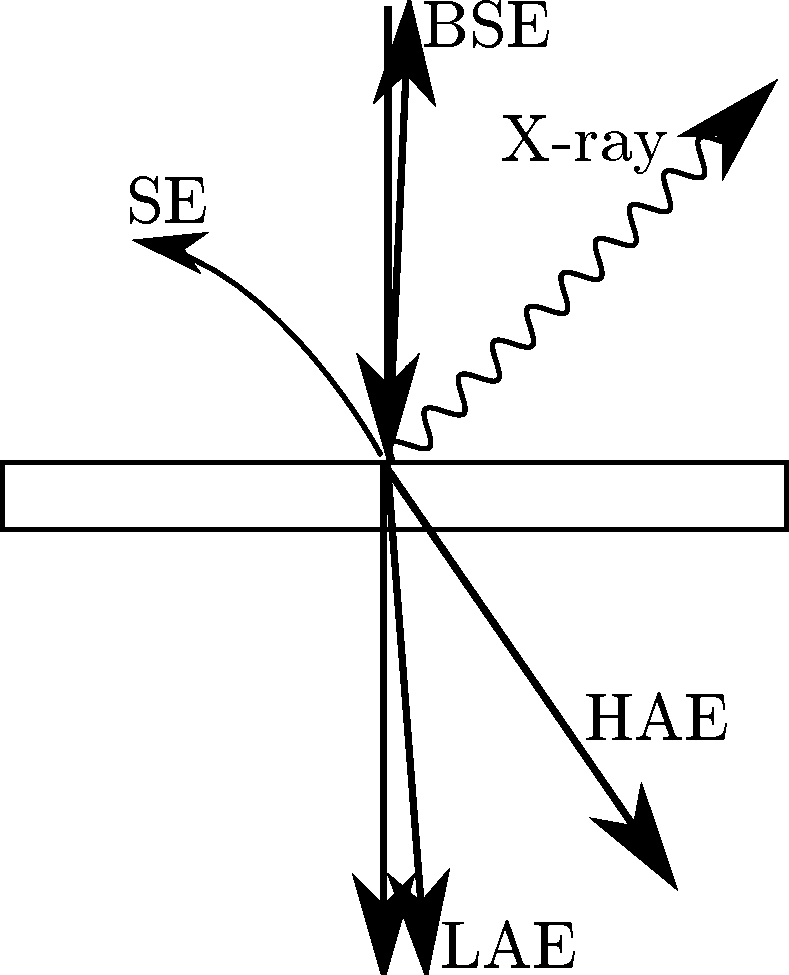
\includegraphics[width=0.5\textwidth]{exp_em_electron_interaction}
 \caption[Electron interactions with materials]{\label{fig:exp_em_electron_interaction}Schematic of an electron beam interacting with a sample showing backscattered electrons (BSE), secondary electrons (SE), generated X-rays, low angle scattered electrons (LAE), high angle scattered electrons (HAE), and the main electron beam passing through the sample.}
\end{figure}

This work relied upon two measurement techniques which utilized electrons as their primary probe, scanning electron microscopy (SEM) and (scanning)transmission electron microscopy (STEM/TEM).
SEM is an invaluable technique non-destructive technique for examining surfaces at high resolution to extract information about both the structural and chemical properties.
STEM/TEM is a tool which uses similar interactions to examine the cross sectional structural and chemical properties of mechanically thinned slices of materials with sufficient resolution to examine individual columns of atoms in crystals.
\subsection{SEM} Scanning electron microscopy is a high resolution non-destructive and non-contact technique used to examine the surface of a sample.
SEM can reveal the topography and chemical composition of a surface down to 10's of nanometers, and the chemical composition on the micrometer scale.
These measurements are achieved through the interaction of a beam of nearly-monochromatic electrons generated from a heated filament or cold cathode and accelerated to kilovolt velocities in an high vacuum chamber and focused onto a sample.
Magnification is achieved in SEM by careful scanning of the focused beam over a small area.

\subsubsection{Secondary Electron Imaging} The most common electron-material interaction utilized in SEM is generation of images through the production and capture of secondary electrons.
Secondary electrons are continuum (valence and conduction band electrons) excited from the sample through inelastic scattering excitations as an electron beam penetrates into a sample.
These electrons typically have energies of less than 50~eV\cite{goldstein2003scanning}.
Secondary electrons, while generated along the path of incoming electrons, can only escape from depths of less than 7.5~nm, making secondary electrons surface sensitive\cite{goldstein2003scanning}.
Secondary electrons are collected by biasing an electron detector to electrostatically attract these low energy electrons while not appreciably affecting the incoming beam.
Electron detectors are typically a phosphor screen combined with a photomultiplier tube to provide high gain.
Images are formed by scanning the beam across the surface of the sample and counting the secondary electron yield for each dwell point within the scan.
The resulting grid of counts is transformed into a bitmapped grayscale image.

As secondary electrons are low energy, their escape depth from a surface is very shallow (\(<\)~2~nm), as such their yield is very sensitive to the local topography of the sample.
Thus to the first approximation, the contrast in a grayscale image formed from secondary electrons is a representation of the topography present on the surface of the sample.
Regions with vertical extent will increase the yield of secondary electrons, due to more of the sample being within nanometers of the surface.
An extreme case of this is vertical edges, which will have a high yield of secondary electrons, due to having the top and side surfaces both yielding secondary electrons.

\subsubsection{Backscattered Electron Imaging} High energy incoming electrons can also interact with samples via elastic scattering.
Electrons which are scattered at close to 90\degree{} are backscattered close to the incoming beam.
By placing unbiased detector near the incoming electron beam the detector can capture backscattered electrons.
The electron elastic scattering process is proportional to atomic mass (\(\sim\)\(\sqrt{Z}\))) of the sample.
The yield of backscattered electrons provides mass (usually called compositional) contrast of the sample under the electron beam.
Penetration depth of the electron beam for backscattered electrons is deeper than secondary electrons, generally penetrating 1--2~\micro{}m into the sample, as well as laterally broadening.
Such broadening reduces the resolution of backscattered imaging compared to secondary electron imaging.

\subsubsection{Practical SEM} The practical application of SEM for imaging of samples requires the optimization of several parameters.
While SEM is a non-destructive measurement technique, intentional sample preparation can vastly improve the imaging resolution and reduce noise.
A key requirement for SEM samples is that the sample is sufficiently conductive to conduct away the electrons delivered by the scanning beam.
For high conductivity samples, sample preparation can be as simple as bonding to a sample holder using conductive tape or paste (such as carbon tape or silver paste).
Samples with poorer bulk conductivity may require conductive paste applied to contact the top surface to the sample holder.
Highly insulating samples are normally coated with a thin layer of high density metal (Pt, Au) or amorphous carbon in order to provide a conduction path to the conductive paste connecting the top surface to the sample holder.

Optimization of imaging for a given sample is achieved through the tuning of several imaging parameters, working distance, accelerating voltage, beam current and dwell time\cite{goldstein2003scanning}.
For typical secondary electron imaging, the goal is to interact with the thin top surface layer with the smallest lateral beam possible.
Minimization of accelerating voltage, beam current and working distance will maximize the resolution and reduce the surface interaction.
Reduction of these working parameters has the side effect of reducing the signal to noise ratio (SNR) of imaging.
Increasing dwell time can improve SNR, but for poorly conductive samples charge buildup will cause deflection of the incoming beam.
Stacked averaging of quick scans yields improved SNR on the tradeoff of time.

Interpretation of the secondary electron images in one key case is ambiguous; topographic features with vertical extent can appear to be both a depression and a bump simultaneously, due to the assumption of the human visual system that lighting always comes from above\cite{goldstein2003scanning}.
Care must be taken for features of this type to avoid misinterpretation.
Modification of some imaging parameters can break the ambiguity and reveal the topography, including tilting the sample, rotating it about its surface normal using the SEM's focus and depth of field parameters to slice through the topography.

Imaging of samples using backscattered electrons to achieve chemical composition requires optimization of the elastic scattering process from the sample.
The primary parameter than improves backscattered electron yield is increases of the electron accelerating voltage.
Increasing the accelerating voltage has the downside of increasing the area of electron interaction, which reduces the effective spatial resolution\cite{goldstein2003scanning}.
The elastic scattering process is less efficient per incident electron than secondary electron generation, as such beam dwell times must be increased to improve SNR\@.
To obtain a accurate measure of chemical composition, samples for backscatter analysis should be as flat as possible, as topography can modify the yield of backscattered electrons, processing such as polishing is essential for the highest accuracy chemical composition.
If the measurement is intended to be non-destructive, careful correlation between backscattered and secondary electron images must be used to ignore topographic effects.
\subsection{TEM} While scanning electron microscopy relies on the information generated from the surface and sub-surface of arbitrarily thick samples, transmission electron microscopy (TEM) relies on the information generated from electrons which transmit through a sample.
Through control of the electron beam information about the thickness, crystalinity and defects of a sample can be collected.

Imaging of samples via TEM is produced via one of several interaction mechanisms of a beam electrons with a thin sample, as noted in the transmitted electron beams in \cref{fig:exp_em_electron_interaction}.
Electron beams are generally on the order 10's to 100's of kilovolts and are controlled via magnetic lenses\cite{Egerton2005}.
Images can be formed by collecting the scattered beam (dark-field) or the transmitted beam (bright-field) focused onto a scintillating screen or electronic CCD array.
Magnification in TEM is achieved by controlling the width of the beam that passes through the sample and then expanding it again onto the detector.
Magnification is generally limited by aberrations present in the magnetic lenses of the system.

Without any specific alignment of the sample, TEM image intensity provides contrast of the thickness-density product of the sample\cite{Egerton2005}.
Electrons are absorbed or scattered away more strongly where there are more atoms present in the path of the electron beam, either through more electrons per unit thickness, or more thickness in total.
Thus, some contrast formed in the image is an indication of the composition.

While thickness-density contrast can provide some information, it is generally useful for amorphous or biological samples.
Crystalline materials offer several other contrast mechanisms.
The de~Broglie wavelength of electrons accelerated in a TEM is much smaller than the spacing between atoms in typical materials, so those electrons can undergo diffraction when they interact with a crystalline sample.
Polycrystalline samples will provide distinct intensity contrast due to their large changes in orientation relative to the incoming electron beam, diffracting varying amounts of electrons\cite{Egerton2005}.

Whens samples are more crystalline, polycrystalline diffraction contrast generally no longer plays a large role.
In order improve the contrast effects of electrons passing through crystalline samples, the sample must be aligned along a ``zone-axis,'' along some crystal direction in order to transport electrons mostly unperturbed down atomic columns.
TEM samples are tilted to align the sample so the beam travels along a crystal direction.
When crystalline samples are aligned in such a way, defects that break the periodicity of the crystal result in phase contrast.
Phase contrast will highlight regions where the atomic columns have defects which scatter electrons\cite{Egerton2005}.

When a sample has crystal defects which present the same zone axis, such as twins, they do not show up in diffraction contrast or traditional phase contrast.
In these cases, single zone axis imaging cannot provide a contrast mechanism which differentiates the two phases.
Two-zone axis contrast tilts the sample in a second direction perpendicular to the first and brings the sample into a dual-diffraction condition.
Since such crystal phases differ in the direction perpendicular to the zone axis, the dual-zone diffraction uses this difference to provide contrast.

Beyond imaging, the electron beam can be adjusted such that after the electrons pass through the sample, the electrons that diffract with the crystal planes can be focused into spots resulting in a diffraction pattern.
This diffraction pattern is akin to an X-ray pattern, it can be used to determine the crystal structure and orientation of the sample under the beam.
The size of the electron beam can also be limited, a method known as selected area diffraction (SAD), allowing examination of sections of the sample.
\subsubsection{Practical TEM} While TEM is a excellent technique for investigating the microstructure of epitaxial thin films, it imposes strict limitations on sample preparation.
Samples must have lateral dimensions of several millimetres while being thinned to electron transparency.
The exact thickness depends upon the density of the material and the TEM conditions.
Samples must be generally thinner than 100~nm for enough electron transmission to provide enough electron scattering to provide contrast while also having those scattered electrons pass through to a detector.

Samples generally start out as wafers or sections of wafers with thicknesses of 500~\micro{}m and lateral dimensions of up to several inches.
Before thinning of a TEM sample can be undertaken, a section of a (possibly) large bulk sample must be selected.
The section selected must be of a size compatible with the thinning process.
Preparation of such sections depends upon the properties of the substrate.
For substrates with good cleaving properties, a thin bar can be cleaved, for substrates which are much harder, bars must be sectioned using sawing methods such as diamond or wire saws.

Once sections have been extracted from a larger sample, they must be progressively thinned.
This is done through a number of steps, starting with mechanical polishing.
In traditional sample preparation a sample is preferentially polished in a wedge shape, providing a gradient of thickness, where at some point the ideal thickness is present.
In modern preparation techniques the sample is ``dimpled,'' creating a sample with circular gradient of thickness and then ion milled until break through.
Samples prepared by most methods are gentle argon ion milled to remove polishing damage.

When preparation of a specific region of a sample is required, traditional preparation techniques do not provide enough spatial specificity to select features at the micro or nano level.
For sample preparation of this type preparation is performed using a Focused Ion Beam (FIB) milling system.
A hybrid gallium beam/SEM system is used to selectively mill the region of interest and perform localized sputtering of a sample, slicing out a section.
After isolating the section, it is welded to a nanomanipulator probe and transferred onto a TEM grid.
The sample is then thinned to electron transparency with the FIB beam, before finally being cleaned by argon gentle ion milling.

Preparation techniques must be extensively experimented with when preparing new or unknown samples.
Some epitaxial layers will have greatly differing mechanical properties and react differently to mechanical polishing and ion sputtering.
Care must be taken to not preferentially remove the material of interest.
Haphazard preparation can result in the introduction of artifacts which may cause misinterpretation during imaging.

Beyond sample preparation, imaging in a TEM can be modified by tuning several parameters.
The accelerating voltage of the TEM affects the wavelength of the electron beam, improving resolution with increasing accelerating voltage\cite{Kohl2008}, however resolution is ultimately limited by lens aberrations.
Lens aberrations can only be improved by the introduction of correctors such as electron monochrometers (which reduce electron current by throwing away those outside a set energy range) and aberration correctors which significantly increase cost.
Beam current control is important to provide good signal to noise, but excess current can cause heating and damage in ultra-thin samples.

\subsection{STEM}
While TEM image formation passes a large beam of electrons through a region of a sample, scanning transmission electron microscopy (STEM) forms an image more akin to SEM\@.
The electron beam is rastered across the thin sample and an image is formed by measuring electron beam current on one of several detectors.
Because the electron beam is a focused point rather than a beam, with the detector immediately after the sample, the maximum resolution achievable in such a system is substantially higher than traditional TEM, reaching levels of \(<\)~1\AA{}.
While STEM's rastering system is beneficial for improving traditional bright-field and dark-field imaging, its major benefit is the addition of the High Angle Annular Dark Field (HAADF) detector for imaging.
The HAADF detector is located after the sample at a larger angular deviation in comparison to the small angle scattering used in TEM, this high angle scattering arises due to atomic Z number scattering of the electrons.
The resulting image formed by collecting data with a HAADF detector is a Z-contrast image, with the brighter spots corresponding to higher Z-number atomic columns within a sample.
The Z-contrast provided by STEM allows identification of atoms within a crystal structure based upon the relative intensities.

In addition to the Z-contrast imaging available within STEM, the electron beam which passes through the sample has energy losses which are characteristic of the atoms which the beam passed.
If a spectrometer is placed below the sample, the energy loss can be measured and a Z-contrast image can be correlated with simultaneous spectroscopic energy loss information, providing chemical pseudo-contrast after post processing.
Such a process is known Electron Energy Loss Spectroscopy (EELS).

\subsubsection{Practical STEM} 
The preparation conditions for STEM is even more onerous than those for traditional TEM\@.
The electron yield for HAADF imaging and EELS quickly diminishes with increasing thickness of the sample.
Samples must be thinned by progressive low energy ion milling to ensure no remaining damage or amorphous layers are present.
Such thin layers must also be stored in vacuum and analyzed quickly as such thin samples can quickly react with water and oxygen in air and chemically react or adsorb contaminants.

STEM imaging is most useful when paired with traditional TEM imaging, as phase and diffraction contrast can highlight regions of interest and Z-contrast imaging can examine the fine details at boundaries between such regions.
Additionally, combining STEM with 2DXRD and careful sample preparation which maintains orientation relationships can provide absolute crystal orientation information, including polarity of polar crystals.

\section{Growth Techniques}
The work presented in this thesis are prepared primarily by two different growth methods, pulsed laser deposition (PLD) and molecular beam epitaxy (MBE).
While these methods are distinct in their properties and the regimes under which they operate, the same material systems were not prepared by both systems, so direct comparisons cannot be made.
Nevertheless, the differences between these growth processes will be examined in some detail to provide sufficient motivation for their choice for the given experiments.
\subsection{PLD} Pulsed laser deposition (PLD) is a versatile method of growing epitaxial thin films and nanostructures.
PLD has the ability to operate in a non-equilibrium growth regime, that is, at a point where the atoms are excited to energies much above the temperature of the growth substrate.
Such a regime is achieved by the use of a pulsed, high photon energy and high energy density laser to produce the atomic species used for growth.
The properties of the PLD growth system allow a wide range of temperatures, pressures and material types to be used during attempts at epitaxial growths.
\begin{figure}
 \centering 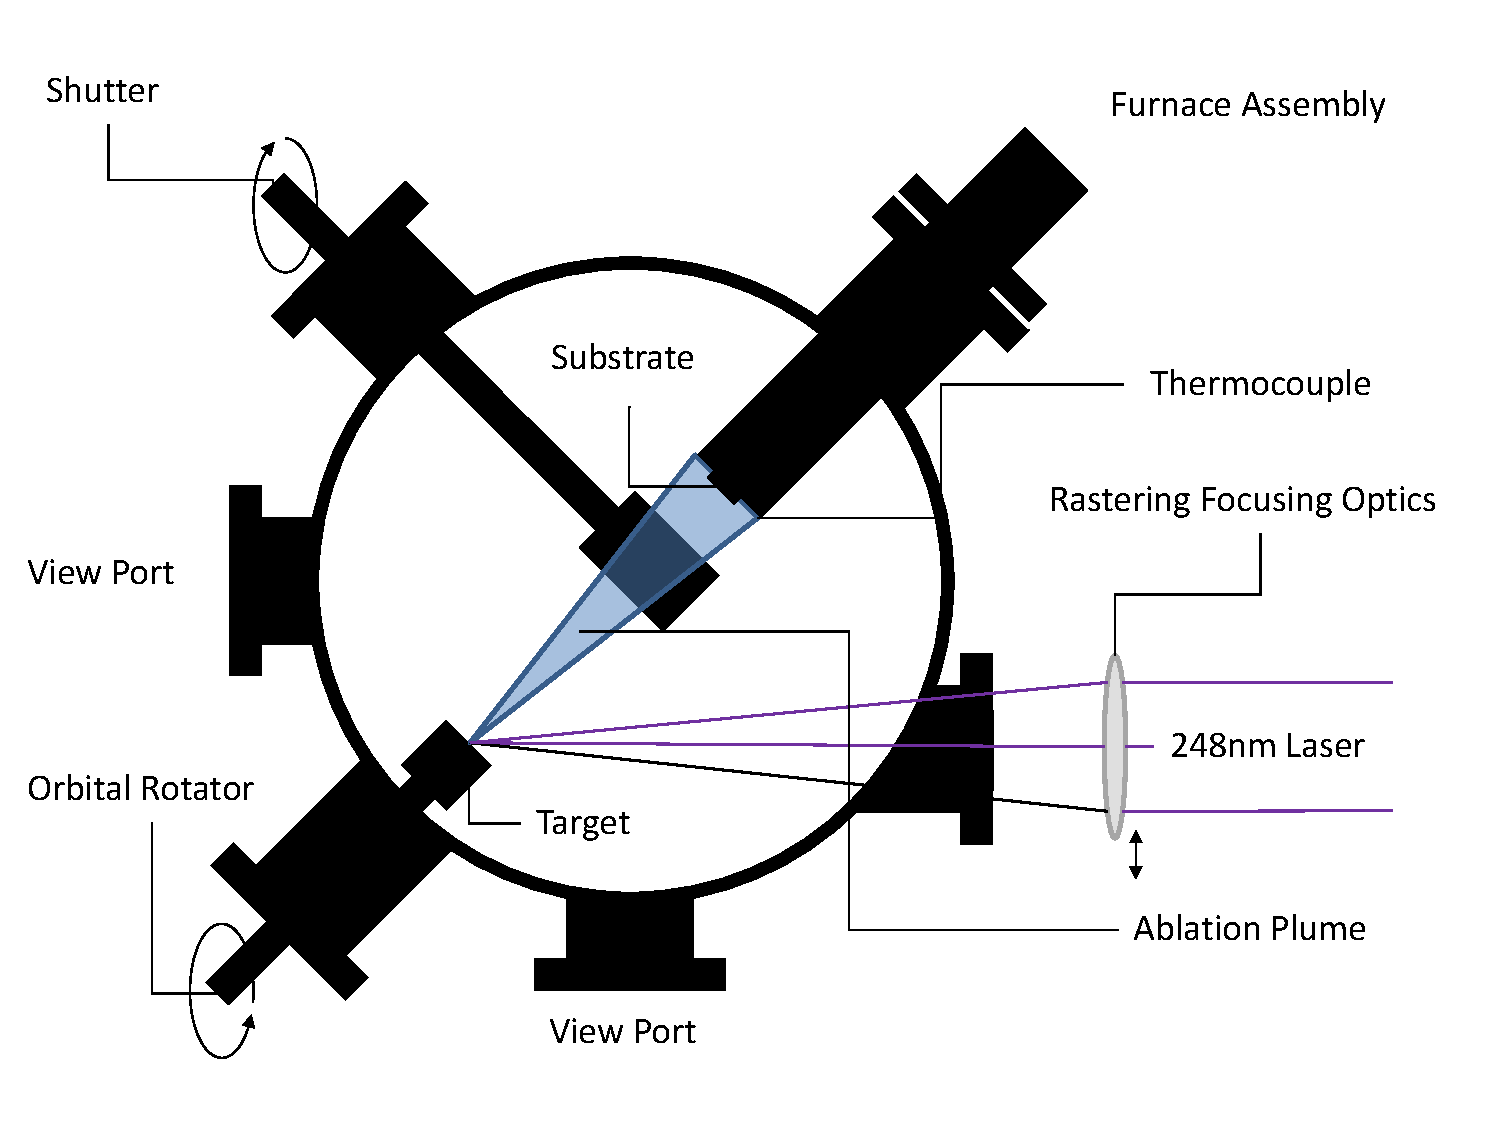
\includegraphics[width=0.9\textwidth]{exp_PLD_chamber}
 \caption{\label{fig:exp_pld_chamber}PLD Chamber Schematic after~\cite{stephen-thesis} (used with permission)}
\end{figure}

The PLD process uses a process known as laser ablation to produce the atomic species used for epitaxial growth.
The laser ablation process relies on several key parameters of the laser and to a lesser extent a few material parameters.
The lasers used in PLD have pulse widths of \(<\)~50~ns, with UV photon energies and total energies of 50---500~mJ/pulse.
Typical PLD lasers are excimer lasers with 248~nm UV photons and pulse widths of \(\sim\)25~ns.
Growth rates for PLD are limited by the pulse rate of the laser, and secondarily by the ability of the target to withstand the sustained energy deposition without melting.

The laser ablation process is achieved by application of laser pulses focused onto a target material, to achieve energy densities \(>\)~1~J/cm\textsuperscript{2}.
The photon energy is absorbed within a thin surface layer 1/\textalpha{}, producing plasmons, excited electrons and excitons\cite{Willmott2000}.
These high energy electrons thermalize and release their energy into the lattice within a few picoseconds.
After this thermalization step, the ablation depth is modified by thermal diffusion, highly conductive metals can quickly spread heat up to a micron deep.
The deposited energy then results in a pulse of evaporation from the target, called the plume.
For highly thermally conductive samples, the surface layer can begin to ablate before laser pulse is fully absorbed, in these cases further absorption in bulk is screened by the atomic plume\cite{Willmott2000}.

Regardless of the target material, a plume is generated at the laser spot which, due to the laser pulse and heating timescales, is stochiometric with regards to the composition of the target.
The atomic plume is also highly ionized, with energies of 1--100~eV and with typical energies of 5--50~eV\@. The atomic plume is now a vapour but highly compressed next to the target surface, explodes perpendicular to the surface, expanding across the deposition chamber, to be collected by a waiting substrate.
The plume expands from the target with a \(\cos^{10-20}(\theta)\)
dependence, meaning it is highly peaked centrally about the spot.
Once the atomic plume arrives at the substrate, its energy is delivered to the growing film.
The high energy atoms, in addition to having high rates of diffusion, also promote the movement of atoms already present by providing activation energy for their diffusion processes\cite{Willmott2000}.
This is a key reason the PLD process can be used at substrate temperatures lower than other methods, the atomic plume delivers energy directly to the growing film.

Due to the generation of atomic species using light, the environment surrounding the target and growth substrate need not be ultra-high-vacuum or even high vacuum for the excited plume to successfully traverse the gap between target and substrate.
Gas pressures on the order of mTorr can be used to modify the energetics of the atomic plume, reducing the total energy or modifying the distribution\cite{Willmott2000}.
The addition of reactive gasses into the chamber, in addition to participating in plume modification, can also participate chemically in the growth process, allowing the growth of oxides and other gas-incorporating materials.
Doping of materials grown with PLD is achievable by incorporating the dopant elements into the existing targets, or by periodically co-abating pure targets using a target exchange system.

The main limitations of PLD are due to the highly peaked nature of the laser plume, the spatial extent of the atomic plume is limited.
The plume must be rastered across large substrate into order to grow a uniform layer.
A secondary limitation is the production of macroscopic droplets which can impact the epitaxial growth process.
The droplets are produced by several processes, some of which can be mitigated.
Targets must be of very high density in order to ensure superheated gasses from voids do not eject pieces of the target.
For highly thermally conductive samples (typically metals), the laser pulse can cause sub-surface boiling, resulting in ejection of liquid material from the target.
For systems which experience this issue, energy per pulse must be reduced to the minimum which can achieve ablation.
A similar process which produces macroscopic droplets is recoil ejection, again for fast conducting materials.
As the vaporization shockwave in a target moves into already melted material, the forces can cause a compression and rebound of the liquid material into a macroscopic droplet.

\subsection{MBE} Molecular beam epitaxy (MBE) is considered the gold standard for the growth carefully controlled epitaxial thin films and nanostructures, being used for both research and commercial purposes.
Its implementation as a growth process allows for a wide range of growth rates from angstroms per second to microns per minute, while controlling the exact ratio of incoming atomic species, and allowing for abrupt changes in composition.

MBE growth systems consist of a large ultra high vacuum (UHV, \(<\) 1e-8 Torr) chamber, along with associated load lock system and exchange hardware and can accept growth substrates of sizes up to several inches.
This low pressure environment is essential to the MBE process to ensure a mean free path of larger than the chamber for the atomic beams used during growth.
These atomic beams are generated in the chamber by one of two processes, effusion cells, or gas sources.
In an effusion cell, a high temperature ceramic containing a solid ultra-pure source of material, is heated to cause evaporation, which then travels in the molecular beam regime across the chamber to a substrate.
Effusion cell rates are controlled by the temperature of the cell.
In gas sources, an organometallic gas containing the atomic species of interest is passed into the chamber via a ``cracker,'' a heated filament used to burn the organic components of the gas, leaving the atomic species which travel across the chamber and are collected on a substrate.
Gas source rates are controlled by mass flow controllers adjusting the rate of gas passing into the system.
Growth rates of angstroms per minute to micrometers per hour are possible via high flow crackers and industrial growths.

MBE systems are used to grow materials in a wide variety of systems, typically concentrated in the III-V, and can also include a wide variety of electrical dopants during growth.
Strict control of the atomic sources allows growth of repeating multilayer stacks, graded materials and quantum structures.
In addition to the careful control of the atomic species, MBE's low pressure system allows in-situ monitoring and characterization of the growth surface using electron-based techniques such as reflection high energy electron diffraction (RHEED).

The main limitation of MBE is the ability to only produce a single sample at a time, making it unsuitable for high volume commercial production.
Another limitation is the heating and temperature control of the substrate.
Since samples must be added via load lock, contact heating and temperature measurement is impractical, leaving only indirect radiative heating and pyrometry temperature measurement.

\part{III-V Materials on Silicon}
\chapter{The Role of Vicinal Surfaces in Epitaxial Twin Formation}
\subsection{Introduction}
Since the microelectronics revolution, Silicon has been a dominant material 
for the production of devices for a variety of applications. Silicon has 
non-ideal properties for a variety of applications but remains dominant due 
to its well-understood processing parameters and large manufacture install 
base, providing economies of scale. The III-V semiconductors offer superior 
properties for a variety of applications when compared to silicon, and are 
actively used in applications were performance is valued above other 
considerations, such as military and space sectors. The goal of integrating 
III-V semiconductors into silicon based microelectronics has spawned extensive 
research into the processing involved to grow or otherwise electronically 
attach these materials with minimal defects.

Under auspices of the ARISE Photovoltaics project, the III-V 
semiconductors GaAs, GaSb, AlSb and InP were grown as thin films under a 
variety of conditions on single crystal silicon substrates, in order to 
examine the growth process and electro-optic properties. The role of the 
varied lattice mismatch, growth parameters, and substrate properties were 
examined and several previously undocumented phenomona were examined due to 
the use of 2DXRD, whose benefits were documented in \cref{sec:2DXRD}.

The formation of epitaxial (or growth) twins was found to be a key area where 
the literature had performed little examination. The role of twins in the 
formation of electronic defect networks, and the effects vicinal (offcut) 
substrates had on their formation were thoroughly examined and a 
explanatory model was developed to explain factors that affect their formation 
and provide proposed routes towards their minimization and 
elimination\cite{Devenyi2011}. This work was completed in close collaboration 
with Ms. Steffi Woo, a Ph.D. candidate in Material Science and Engineering and 
McMaster, with the TEM/STEM work performed exclusively by her and all other 
work being collaborative.

\subsection{Background}
\todo{Should a section covering the background of III-V on Silicon go here, or 
go into the introductory material at the beginning of the thesis}

\subsection{Experimental} \todo{This section is currently copy-pased from 
paper, is this appropriate?}
Semiconductor thin films (GaAs, InP, GaSb, and AlSb) were deposited on nominal 
(001)-oriented ($\pm$0.5$^\circ$) and vicinal Si substrates (offcut 
4.7$^\circ$ ($\pm$0.25$^\circ$) towards [110]) using a SVT Associates 
molecular beam epitaxy (MBE) system. As-received epi-ready wafers were cleaned 
for 1 min in a 4\% HF in deionized (DI) water dip followed by a 30 sec DI 
rinse immediately prior to their insertion into the MBE load-lock. Before film 
deposition, both the nominal and vicinal Si(001) substrates underwent a 15 min 
degassing procedure at 350~$^\circ$C followed by a thermal treatment at 
800~$^\circ$C for up to 5 min, in order to reconstruct the Si surface into 
single domain 
terraces\cite{NeergaardWaltenburg1995,S1991,Sakamoto1986,Pehlke1991}. A small 
number of single steps are expected to remain on vicinal substrates, a higher 
number on nominal substrates because of the larger terrace length. Growth 
conditions followed established 
protocols\cite{Akahane2004,Balakrishnan2006a,Fischer1986} and yielded 
comparable rocking curve full-width half-maximum for the [004] reflection 
using double crystal X-ray diffraction. AlSb thin films were grown to a 
thickness of 550~nm with a 20~nm GaSb capping layer to avoid oxidation. GaAs 
thin films was grown to a thickness of 600~nm and GaSb to a thickness of 
500~nm. InP samples were grown at 470~$^\circ$C with a V/III flux ratio of 2 
at a growth rate of 1 $\mu m$/hr, resulting in a thickness of 600~nm. Double 
crystal X-ray and TEM data also revealed that all films are fully relaxed by a 
network of interfacial misfit dislocations\cite{Vajargah2011}. GaSb samples 
were grown in the presence of a 5 nm AlSb buffer layer, as prescribed by 
Akahane \textit{et al}.\cite{Akahane2004}.

Stereographic pole figures were generated for each sample using 2DXRD 
techniques. A Bruker SMART 6000 CCD detector on a Bruker 3-circle D8 
goniometer (Bruker AXS Inc., Madison, WI) with a Rigaku RU-200 rotating anode 
X-ray generator (Rigaku MSc, The Woodlands, TX) and parallel-focusing 
monochromator optics was used for the data collection. Scans were taken with 
the detector centered on the (111) 2$\theta$ of the material of interest and 
the sample rotated through 360$^\circ$ in 0.5$^\circ$ increments about the 
surface normal of the sample. A 1D integration of all frames was used to 
determine the combined width of the (111) peaks using MAX3D software (McMaster 
University)\cite{Britten2007}. The peak width was then used to integrate (111) 
reflections from all frames, including a background and absorption correction 
for the corresponding material with GADDS (Bruker-AXS) software, resulting in 
a pole figure. Pole intensities were obtained from pole figures using a 
circular integration cursor with a 10 pixel radius which was centered on the 
pole so as to maximize the total intensity captured. All pole intensities were 
corrected for structure factor and frame exposure times.

For each sample two \{110\} TEM cross-sections were prepared, one parallel to 
the [110] miscut direction and the other perpendicular. The specimens were 
prepared by the standard procedure of mechanical polishing, dimpling, and 
ion-milling (4 keV Ar-ions at an incident angle of $\pm$4$^\circ$ using a 
liquid nitrogen cold stage for InP) until perforation. Crystallographic 
information of the epitaxial layer was obtained using diffraction contrast 
imaging with a Philips CM12 conventional transmission electron microscope 
(TEM) operated at 120 kV and equipped with a LaB$_6$ filament. In addition, 
electron diffraction analysis was performed using selected area electron 
diffraction (SAD).
\subsection{Results}
2DXRD measurements performed on as-grown thin films indicated a bulk 
orientation of the material consistent with epitaxial alignment with the 
single crystal silicon substrate. The pole figures generated from 2DXRD data, 
such as \cref{fig:twins_pole_example} also contained a number of other peaks 
at reduced intensity indicating other orientations of the material of interest 
other than the bulk orientation. In order to develop a comprehensive picture 
of the distribution of the grown thin films, simulated pole figures were 
examined in an attempt to generate a composite pole figure which qualitatively 
matched the figures generated from data. Based on these simulations, the 
simulated pole figure \cref{fig:twins_sim_polefigure} was developed, 
indicating that the thin films consisted of a bulk epitaxial phase, and four 
primary twin phases, along with secondary twin phases (not shown). The primary twins form 
along (111), (1$\overline{1}$1) ($\overline{1}\overline{1}$1) and ($\overline{1}$11) 
habit planes.
\begin{figure}
    \begin{subfigure}[b]{0.5\linewidth}
        \centering
        \missingfigure{Representative Single Pole Figure}
        \caption{A representative pole figure of GaAs grown on nominal (100) 
        Silicon\label{fig:twins_pole_example}}
    \end{subfigure}
    \begin{subfigure}[b]{0.5\linewidth}
        \centering
        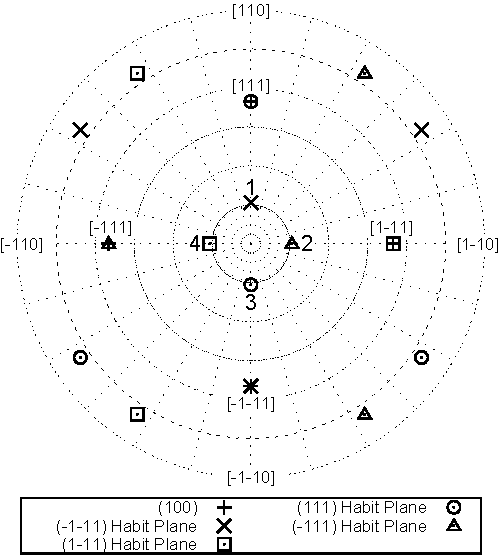
\includegraphics[width=\textwidth]{twins_sim_polefigure}
        \caption{Simulated III-V on silicon pole figure. Unique markers are used 
        for later intensity measurements.\label{fig:twins_sim_polefigure}}
    \end{subfigure}
    \caption{\label{fig:polefigure_example}Represenative pole figure and simulated pole 
    figure}
\end{figure}

Growths of III-V thin films were performed on vicinal substrates due to the established 
literature indicating the ability of atomic height steps formed by such substrates to 
overcome the polar-on-non-polar growth problem\cite{Kroemer1987}. The pole figures 
generated for thin films grown on vicinal substrates were found to have a distinctive 
asymmetry in the intensity distribution of the peaks associated with twinned orientation, 
when compared to the thin films grown on nominal silicon substrates. The pole figures for 
both nominal and vicinal pole figures for the III-V thin films are shown in 
\cref{fig:twins_polefigure}.

\begin{figure}
    \centering
    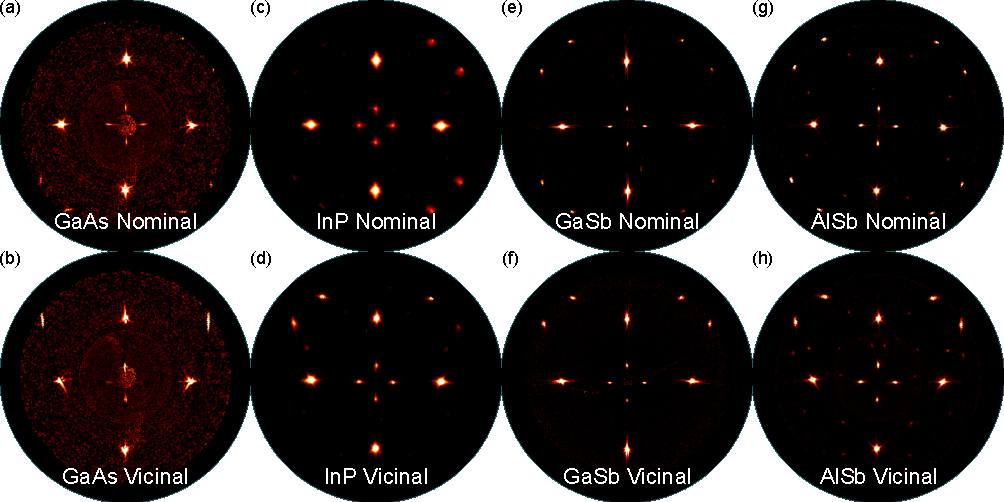
\includegraphics[width=\textwidth]{twins_polefigure}
    \caption{Stereographic \{111\} pole figures generated from 2DXRD show a bulk (100) 
    phase plus four twinned variants as identified in \cref{fig:twins_sim_polefigure}. 
    Twin variant intensity is asymmetric for vicinal 
    substrates.\label{fig:twins_polefigure}}
\end{figure}
\chapter{Tilted Epitaxy on (211) Oriented Substrates}
\section{Introduction}
In parallel to the investigations of vicinal (100) substrates, the ARISE project investigated alternative substrate orientations including (111) and (211). While the results of (111) substrates were uninteresting, growth of thin films on (211) substrates demonstrated a number of interesting properties. Most interesting amongst these was the spontaneous tilting of thin films grown on top of (211) oriented silicon substrates. Such tilting had been remarked upon previously in literature,  but no comprehensive examination of its origins or relationship to material parameters had been examined.

In this work, also done in close collaboration with Ms. Steffi Woo, the spontaneous 
tilting of thin films grown on (211) oriented silicon substrates was examined. The 
effects of the naturally asymmetric substrate was found to cause a tilt of the growing 
thin film in order to minimize the strain across the interface. Using this idea of 
projected strain minimization across the interface, a model was developed which predicted 
the tilt as a function of intrinsic lattice mismatch between the substrate and thin film. 
Examination of the reports of thin film tilting in literature showed the model 
successfully calculated tilt for a large number of material systems and made predictions 
for those systems for which no measured values had been reported.
\section{Background}
The (211) orientation of non-polar semiconductor substrates, most notably silicon, has a number of beneficial properties. Of most relevance to the epitaxy of thin films on Si(211) substrates is the occurrence of two energetically non-equivalent lattice sites on the surface, without the need for surface reconstruction.\cite{Wright1982} These two non-equivalent lattice sites offer preferential nucleation locations for the individual adatoms during growth of polar (group III-V and II-VI) semiconductors. Such preferred nucleation is proposed to eliminate the occurrence of anti-phase domains (APDs) during the growth of polar semiconductors\cite{Wright1982} while also maintaining the interface neutrality condition of h$\pm$k$\pm$l$=$0.\cite{Wright1982} The intrinsic asymmetry of the (211) surface is also expected to influence the formation of epitaxial twins during growth\cite{Devenyi2011}. Si(211) substrates have been used to produce the highest quality CdTe\cite{Zhao2011}, ZnTe\cite{Wang2011a} and HgCdTe\cite{Dhar1997a} despite large lattice mismatches of 19.4\%, 12.3\%, and 19.1\%, respectively. 

Thin films grown on (211) substrates have been previously observed in literature to have a tilted epilayer orientation relative to the substrate.\cite{Zhao2011,Wang2006,Dhar1997a,Lange1991,Nakamura1992} The tilt phenomenon has been attributed to a number of causes by different authors including the glide and interactions of misfit dislocations \cite{Olsen1975,Riesz1994,Ayers1991,Johnson2011} and localized distortion of the lattice at the interface.\cite{Sasaki1992} The mechanisms proposed thus far have been unsuccessful at predicting the tilt of mismatched epilayers over large range of mismatch (0--20\%) found in III-V and II-VI material systems. A phenomenon intimately intertwined with tilted epitaxy is ``dual epitaxy'', observed by numerous authors\cite{Li1995a,Nakamura1992,Rujirawat1998,Lange1991} that mismatched CdTe on GaAs(211) epitaxy can result in films growing in a twinned orientation, combined with a tilt; such that the (133) planes make up the epilayer surface and are parallel to the substrate (211) planes. The tilt component of dual epitaxy is same tilt phenomenon examined here.

\section{Experimental}
GaSb thin films were deposited on nominal (211)-oriented Si substrates, according to our 
previously published procedures\cite{Devenyi2011}, at 600, 640 and 500{\degree}C. Two 
dimensional X-ray diffraction (2DXRD) frames were captured for stereographic pole figure 
analysis and crystallographic indexing as per Devenyi \textit{et al.}\cite{Devenyi2011}.
\begin{figure}
    \centering
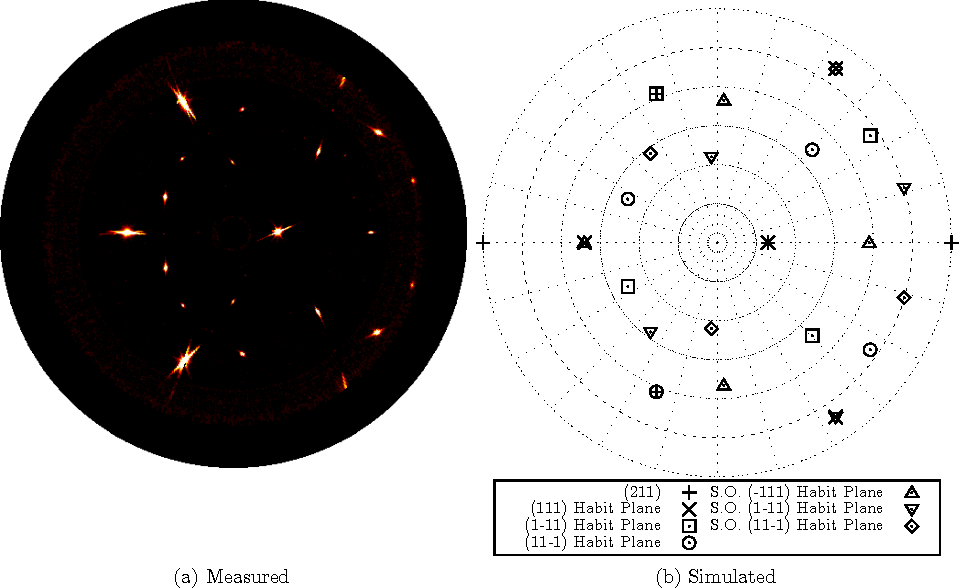
\includegraphics{211_polefigure}
\caption{\label{fig:211_polefigure}a) 2DXRD Stereographic pole figure and b) accompanying modelled pole figure, identifying the origin of each peak in the pole figure from the bulk or one of six twin variants. Overlapping peaks indicate twinning habit planes. Outermost poles are partially visible due to experimental limitations. Streaking in peaks is due to instrumental broadening. (S.O. = second-order twinning).}
\end{figure}
\section{Results}
2DXRD data was processed into a GaSb (111) pole figures as shown in FIG.~\ref{fig:211_polefigure}, representing a stereographic projection of all $<$111$>$ spacings present in the GaSb epilayer. Modeling (as per Devenyi \textit{et al.}\cite{Devenyi2011})\ of the poles present indicate that there are seven phases of GaSb, the bulk (211) orientation of GaSb and six twin variants, three first-order twins and three second-order twins from the twin variant with (111) habit plane, with 58\%, 21\% and 2\% of the intensity (and hence volume fraction) present in the twinned orientation for the films presented here. Volume fractions were determined by integration of the sum of intensity of unique (111) X-ray peaks from all twinned orientations, and divided by total intensity of all unique (111) reflections (sum of bulk and twin intensities), performed using \textit{Bruker GADDS}. There are two distinct nomenclatures used in literature to describe phases present in epitaxial films.\cite{Kim2010a,Lange1991,Johnson2011,DeLyon1995} One method describes the crystallographic direction which is normal to the surface for each phase, while the other (which the authors choose to employ here) describes the nature of the crystallographic orientation relationship between the secondary phases with respect to the orientation of the substrate. Where reference is made to literature using the first, descriptions will be translated into the second for ease of comparison.

Indexing of the crystal unit cells present in the film was performed using \textit{Bruker APEXII} single crystal refinement software, to obtain orientation matrices for the Si substrate as well as the seven GaSb phases. The bulk thin film orientation matrix was then compared to the substrate matrix and a tilt calculated using \textit{orilib} a crystal orientation calculation library, yielding a tilt of 2.65\degree, 2.55\degree and 2.40\degree $\pm$ 0.2\degree about the [01$\overline{1}$] direction towards [$\overline{1}$11], these values are indistinguishable within experimental error. The (111) habit plane twin formed in these films is also tilted with respect to the substrate, by the same angle as the bulk, this is expected by crystallography, since this twinned orientation shares extended interfaces with the bulk orientation.
\begin{figure}
    \centering
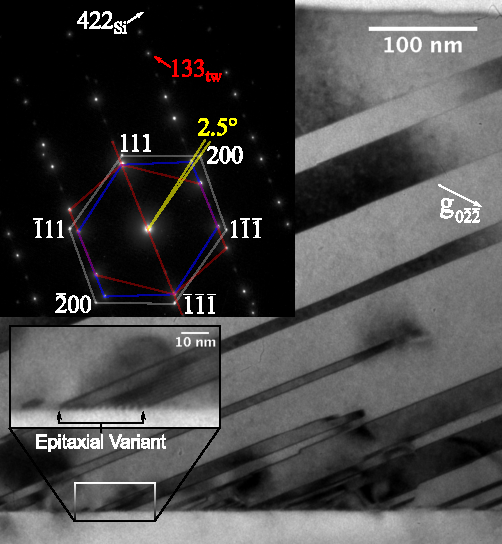
\includegraphics{211_tem}
\caption{\label{fig:211_tem}Conventional TEM image of the (0$\overline{1}$1) cross section, with inset diffraction pattern of the epitaxial and (111) habit plane twin variant in blue and red, respectively, and inset higher-magnification of the epitaxial variant showing misfit dislocations.}
\end{figure}

Two transmission electron microscopy (TEM) cross-sections were prepared, in orthogonal directions of [0$\overline{1}$1] and [1$\overline{1}\overline{1}$]. The specimens were prepared by conventional mechanical polishing and ion milling, and examined as described in Woo \textit{et al.}\cite{Woo2012} Conventional TEM imaging of the (0$\overline{1}$1) cross-section of the epilayers, combined with the selected area electron diffraction (SAED) pattern of the [0$\overline{1}$1] zone axis as shown in FIG.~\ref{fig:211_tem} confirms the presence of microtwins with (111) habit planes. These microtwins are observed in the perpendicular (1$\overline{1}\overline{1}$) cross-section as large bands lying parallel to the interface over a long-range, alternating with the epitaxial variant (not shown). The observed misorientation between the GaSb and Si reflections in the [0$\overline{1}$1] SAED pattern also indicate a tilted epilayer (both epitaxial and twin variants) with a tilt of 2.54$^\circ \pm 0.2^\circ$ towards the [$\overline{1}$11] direction. The 133 reflection of the twinned GaSb nearly coincides with the Si substrate normal 422 reflection. The GaSb twin variant can be differentiated in real space by selective dark-field imaging formed using one of the twinned reflection spots. The jagged features at the GaSb/Si interface (seen in detail in the inset of FIG.~\ref{fig:211_tem}) only belong to the epitaxial variant. This is indicative of the presence of misfit dislocations at the portions of the interface where the epitaxial region meets the substrate, as characterized by Vajargah \textit{et al.}\cite{Vajargah2011b}
\section{Discussion}
Analysis using an atomic ball-and-stick model, along with trigonometric modelling of lattice plane spacing, can be used to demonstrate that the tilted epitaxy reduces the projected in-plane lattice strain along one dimension for the GaSb/Si system. FIG.~\ref{fig:211_model} shows the alignment of planes present in the epitaxial and twinned variants of the GaSb epilayer. The Si(111) plane spacing (in red) at an angle of 19.471\degree to the Si(211) surface is aligned to the GaSb(111) plane spacing (in blue), by a tilt of 2.50\degree in the epilayer. The relationship describing zero projected strain condition between these planes across the interface is described in EQN.~\ref{eqn:211_epi} for the case of $a_{Sub} = a_{Si}$ and $a_{Film} = a_{GaSb}$, where $\delta$ is the tilt angle. This relationship (dot-dash line) also applies over the full range of common heteroepitaxial lattice mismatches grown on (211) substrates, from GaP/Si to CdTe/Si, as shown in FIG.~\ref{fig:211_data}.
\begin{gather} 
 \frac{ a_{film}}{\sqrt{3} \sin(19.471^\circ + \delta)} = \frac{a_{Sub}}{\sqrt{3}\sin(19.471^\circ)} \label{eqn:211_epi}\\
 \frac{ a_{film}}{2\sin(74.207^\circ + \delta)} = \frac{ a_{Sub}}{\sqrt{3}}   \label{eqn:211_twin}
\end{gather}
\begin{figure}
    \centering
\includegraphics{211_model}
\caption{\label{fig:211_model}Ball-and-stick atomic model of a triple junction of the epitaxial orientation, twinned orientation (with (111) habit plane in blue), and the Si(211) surface. Geometrical alignment of the atomic planes as described by EQNs.~\ref{eqn:211_epi} and \ref{eqn:211_twin} are also shown in red/blue and black, respectively. Terrace (T) and edge (E) atom labels denote the two non-equivalent surface sites.}	
\end{figure}
\begin{figure}
    \centering
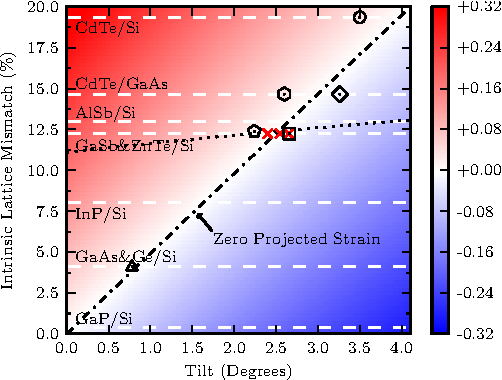
\includegraphics{211_data}
\caption{\label{fig:211_data}Colormap showing the projected strain as a function of 
intrinsic lattice mismatch and positive tilt angle of an epitaxial film, computed from 
EQN.~\ref{eqn:211_epi} with the zero projected strain contour highlighted (dot-dash 
line). The dotted line also overlays EQN.~\ref{eqn:211_twin}. Experimental data points 
from this work ($\times$), Ref.~\textcite{Zhao2011} ($\odot$), Ref.~\textcite{Wang2011a} 
($\boxdot$), Ref.~\textcite{Johnson2011} ($\Diamond$, $\bigtriangleup$) and 
Ref.~\textcite{smith2012_znte,smith2012_gaas} ($\pentagon$, $\varhexagon$) are shown, 
indicating good agreement with measured tilts of thin films. Common heteroepitaxial 
systems are also highlighted. Close lattice mismatches are merged for figure clarity.}
\end{figure}
In the twinned orientation, the Si($\overline{1}$11) plane spacing is aligned to the projection of the GaSb(200)$_{tw}$ plane spacing (both in black) onto the GaSb/Si interface, by a tilt of 2.22\degree. The geometrical constraints of these planes can be described by the relations as expressed in EQN.~\ref{eqn:211_twin}. The line of zero projected strain for the twinned region is also shown in FIG.~\ref{fig:211_data} (dotted line). The applicability of EQN.~\ref{eqn:211_twin} is considerably more limited across heteroepitaxial systems, as the constraints described by EQN.~\ref{eqn:211_epi} also needs to be simultaneously satisfied as extended interfaces are shared. However, an equivalent relationship describing another set of planes for other lattice mismatches may replace the relationship described by EQN.~\ref{eqn:211_twin}. The proposed ball-and-stick atomic model (FIG.~\ref{fig:211_model}) also shows that the Ga- and Sb-atoms in the twinned variant are perfectly registered with the terrace (T) and edge (E) atoms of the Si substrate. The epitaxial variant interface is significantly distorted, and the same atomic registration of Ga- and Sb-atoms to the underlying Si substrate does not occur, however the projected sublattice is still aligned. This correlates well with the misfit dislocations observed at the GaSb/Si interface in the inset of FIG.~\ref{fig:211_tem}.

For general case of an epilayer with unknown twin volume-fraction, the tilt is bounded by competing factors of minimizing strain in both the epitaxial and twinned variants (as in GaSb on Si), with the projected strain effectively minimized at the volume-fraction weighted average of the two tilts. For GaSb with 58\%, 21\% and 2\% twin fraction, the predicted tilts are 2.493\degree, 2.498\degree and 2.500\degree. This small variation in tilt angle is due to the steeper slope of EQN.~\ref{eqn:211_epi}, thus its contribution dominates the weighted average. The intrinsic +12.2\% lattice mismatch between GaSb and Si is minimized, however there are localized strain variations between the epitaxial and twinned regions. For a film with 58\% twin, the projected (111) d-spacing in the epitaxial region is +0.03\% (in compression), while the projected GaSb(200) and Si($\overline{1}$11) d-spacing in the twinned region is -0.12\% (in tension). Thus, the proposed driving force for the tilted epilayer during growth is the minimization of lateral strain of close-packed (111) planes (red/blue planes in FIG.~\ref{fig:211_model}), in one dimension within the two-dimensional projected interface net.

In addition to accounting for the tilt observed for GaSb on Si, this model predicts the tilts observed in several other material systems. The growth of CdTe on Si(211) and GaAs(211) is a common use to buffer the growth of HgCdTe for detector applications. Several authors\cite{Triboulet2009,Yu1999,Lange1991} published results which indicate CdTe epilayers which are tilted in the range of 3.5\degree on Si(211)\cite{Zhao2011} and 3.26\degree on GaAs(211)\cite{Johnson2011}, about the [01$\overline{1}$] direction towards [$\overline{1}$11]. The direction and magnitude reported by those authors agrees well with the tilt of 3.97\degree and 3.00\degree, respectively, as predicted by this model. Discrepancy between the predicted and reported value of tilt is expected to be partially due to the presence of twinning in the epilayer, along with uncertainty in the reported values.

ZnTe is often used as an intermediate buffer epilayer, prior to the growth of CdTe and HgCdTe on Si(211).\cite{Zhao2011,Dhar1997a} Wang \textit{et al.}\cite{Wang2011a} published results which indicate epilayer tilts in the range of 2.66\degree while Smith \textit{et al.}\cite{smith2012_znte} reports tilts of 2.24\degree. This is in good agreement to the predicted value of 2.50\degree obtained from the proposed model. The good matching between our predicted and the reported values of tilt in ZnTe on Si(211) is expected to be due to the substantially low degree of twinning observed.

The model also makes a prediction of the tilt expected from the growth of GaAs on Si(211), a value of 0.83\degree is predicted. A tilt of 0.781\degree is reported by Johnson \textit{et al.}\cite{Johnson2011} when grown alone, and 0.835\degree when capped subsequently with CdTe, again demonstrating good agreement with the model.

For the systems AlSb/Si, InP/Si and GaP/Si, the model predicts tilt angles of 2.65\degree, 1.64\degree and 0.07\degree. Measurements of these material systems are expected to yield tilts that quantitatively follow this model.
\section{Implications for Symmetry and Energy at Epitaxial Surfaces}
The natrually asymmetric (211) surface of cubic non-polar semiconductors offers a alternative route to breaking the symmetry for epitaxial growth. The (211) surface offers two unique properties which can enhance nucleation and growth of lattice mismatched thin films, it's asymmetric surface offers a energy landscape offering different bonding locations, and it's surface has a naturally stepped nature.

The two non-equivalent surface sites present on an unreconstructed (211) surface offer an energy landscape which encourages the nucleation of the polar adatoms. Such a preferred nucleation of adatoms into the two non-equivalent sites results in the natural elimination of anti-phase-domains.

The surface of (211) oriented semiconductors, in addition to having non-equivalent sites, also has a naturally asymmetric surface, consisting of 
\part{Semiconductors on Oxide Substrates}
\chapter{CdTe Growth on Sapphire Substrates and Liftoff Phenomenon}
\section{Introduction}
The growth of CdTe on oxide substrates, specifically single crystal sapphire, has been a 
region of great interest for the Preston research group. Work has been published on 
optimization of growth parameters, the role of lattice constants, and the optical 
properties of the resulting thin films\cite{svetlana-work,stephen-paper}.

While the work investigating the growth parameters and properties of the resulting thin 
films has progressed to a high level, relatively less investigation has been focused on 
explaining the surprising success that has been achieved with this material system. With 
a relative lattice mismatch of 3.xx\% between CdTe and sapphire, a difference in the 
crystallographic space group (cubic CdTe versus hexagonal sapphire), and a vast chemical 
difference (high ionicity semiconductor CdTe versus complex oxide sapphire), the high 
quality single crystal nature of the grown thin films is far from expected.

In this work investigating the CdTe on sapphire heteroepitaxial material system, the 
unexpected high quality growth is examined through the lens of symmetry and energy at the 
epitaxial 
interface. These examinations reveal theoretical support for an explanatory model of the 
epitaxial alignment 
and defects present in CdTe thin films. These examinations also reveal the previously 
undocumented and highly surprising result that CdTe is not bonded nearly as strongly as 
expected to the sapphire substrates after epitaxial growth, resulting in the 
technologically relevant liftoff phenomenon. The liftoff phenomon is examined and its 
resulting freestanding thin films are characterized. This liftoff phenomon has been 
discovered to be significantly robust as to apply for a provisional patent\cite{patent}. 
This work was completed in collaboration 
with Mr. Stephen M. Jovanovic (growths), Dr. Kristoffer Mienander (DFT, surfaces) and Ms. 
Steffi Woo (TEM), and relies on prior work by Dr. Robert Hughes and Dr. Svetlana Neretina.

\section{Background}
CdTe is a cubic semiconductor (a = 6.14xxx) with a very strong propensity to grown 
(111)-up, that is 
alternating layers of cadnimum and telurium, regardless of the structure of the 
underlying substrate. Thus the key requirement for the growth of quality single crystal 
thin films is to control the nucleation and in-plane orientation. \textalpha-Al$_2$O$_3$ 
(sapphire) 
is a rhobehedral complex oxide (a = xxxx, c = yyy), which presents a hexgonal surface net 
on its c-plane surface. As had been previously investigated by the Preston research 
group, the (110) diagonal of CdTe matches to a lattice constant of sapphire to within 
3.xx\%, providing a geometric template for the epitaxial alignment of (111)-up on the 
c-plane surface. While the c-plane sapphire offers an epitaxial template for the CdTe, 
the mismatch of cubic on hexagonal symmetries offers two equivalent orientations for the 
CdTe crystal, as shown in \cref{fig:cdteliftoff_geometry}.
\begin{figure}
    \centering
    \missingfigure{Triangle on Hexagon Fit}
    \caption{\label{fig:cdteliftoff_geometry}Geometric model of cubic CdTe crystal 
    structure fit on hexagonal c-plane sapphire surface}
\end{figure}
Despite the geometric equivalence of two orientations of cubic on hexagonal symmetry, 
growths done by this research group have resulted in a single orientation of CdTe on the 
sapphire surface. Previous work by this research group attempted to explain the preferred 
orientation through experiments in the modification of sapphire\cite{Neretina2009b}, 
suggesting that the energy considerations at the surface play a key factor in epitaxy.
\section{Experimental}
CdTe thin films were deposited on single crystal c-plane \textalpha-Al$_2$O$_3$ $\pm$ 
0.5\degree wafers, obtained from MTI Crystals Inc and diced into 12 mm $\times$ 12 mm 
squares. Prior to deposition, substrates were solvent cleaned in an ultrasonic bath. 
Samples were loaded into a custom pulsed laser deposition chamber at a base pressure of 
1x10E-7 Torr and in-situ annealed at 450\degree\celsius for 30 minutes. CdTe thin films 
were deposited by pulsed laser deposition using a GSI Lumonics IPEX-848 KrF excimer laser 
with a wavelength of 248 nm. Pulses from the laser were focused and rastered radially 
onto a rotating CdTe 2.54 cm diameter target with a spot size of 4.25 
mm\textsuperscript{2} and average 
energy density of 1.8 J/cm\textsuperscript{2}. The CdTe 5N (99.999\%) pressed powder 
target obtained from 
Princeton Scientific was stoichiometric and undoped. During growth samples were kept at a 
nominal temperature of 300\degree\celsius via a Pt-Rh thermocouple on the growth furnace 
surface. 
Films were grown to a thickness of 100 nm, as determined by optical and stylus 
profilometry.

Structural information was obtained using 2DXRD techniques. A Bruker SMART6000 CCD 
detector on a Bruker 3-circle D8 goniometer with Rigaku RU-200 rotating anode X-ray 
generator and parallel-focusing mirror optics were used for the data collection. 2DXRD 
data was processed into pole figures using Bruker GADDS.
\section{Results and Discussion}
CdTe thin films had been previously thoroughly structurally characterized via 2DXRD, AFM 
and TEM. As such, one of the next steps to fully characterize the CdTe thin films was to 
produce larger uniform films\cite{stephen-thesis} and to electrically characterize films 
via resistivity and hall effect. As part of this investigation, lithographic patterning 
of Pt contacts was performed to create van der pauw geometry. Upon performing the acetone 
soak, as the photoresist dissolved, and the metal film floated off the sample, it 
remained in one piece, lifting off the areas of CdTe that were in contact with the metal from the epitaxial substrate. 
For a sample that had been previously characterized to be single crystal, this result was 
unexpected, as all that was required for this liftoff was an ultrasonic bath.
\begin{figure}
    \centering
    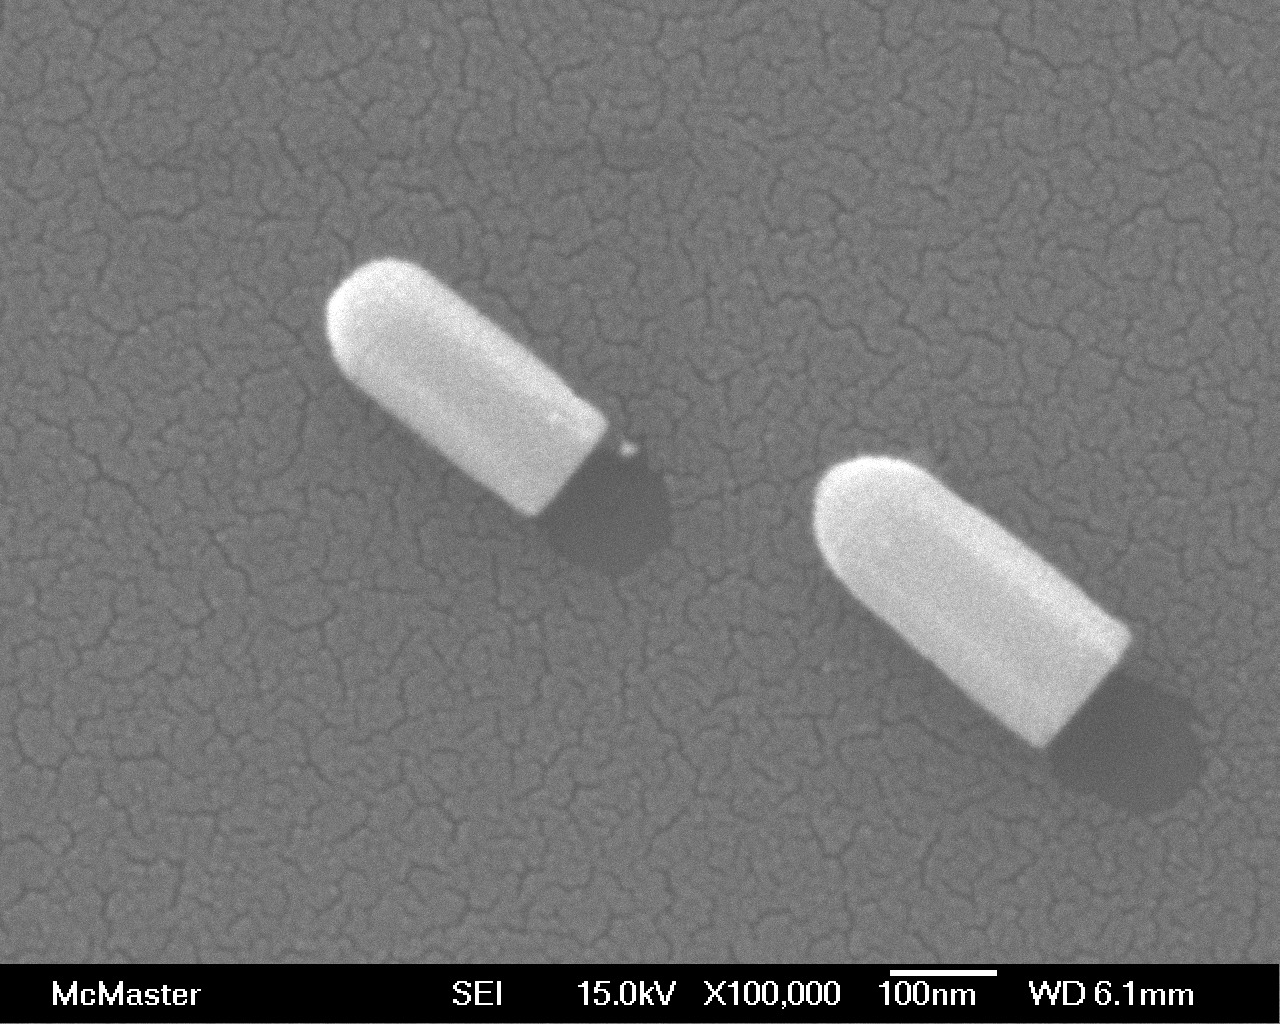
\includegraphics[width=0.8\textwidth]{cdteliftoff_nanowires}
    \caption{\label{fig:cdteliftoff_nanowires}}
\end{figure}
This weak bonding phenomenon had been previously hinted at when CdTe nanowires were 
observed in SEM to have toppled in place, as shown in \cref{fig:cdteliftoff_nanowires}, a 
event that could not have happened unless the bond strength with the interface was very 
weak.

After the discovery of the liftoff phenomenon with lithographic patterning, simpler 
methods of liftoff were attempted. Strong adhesive tapes were found to successfully 
remove thin films with a simple mechanical peeling motion. While the tape peeling was 
effective, the large curvatures cause cleaving and breakage in the lifted off film. 
Adhesive epoxies were attempted and found to provide a more rigid carrier, eliminating 
cleaving and breakage. Yields of liftoff are highly dependent on the quality of bonding 
to the CdTe surface, clean surfaces and effective adhesives are key. Numerous other 
bonding methods were tested including optical element adhesive, polymer films and the 
simplification of liftoff by the addition of LN\textsubscript{2} as thermal shock. The generalized adhesive based liftoff process is shown in \cref{fig:cdteliftoff_process}
\begin{figure}
    \centering
    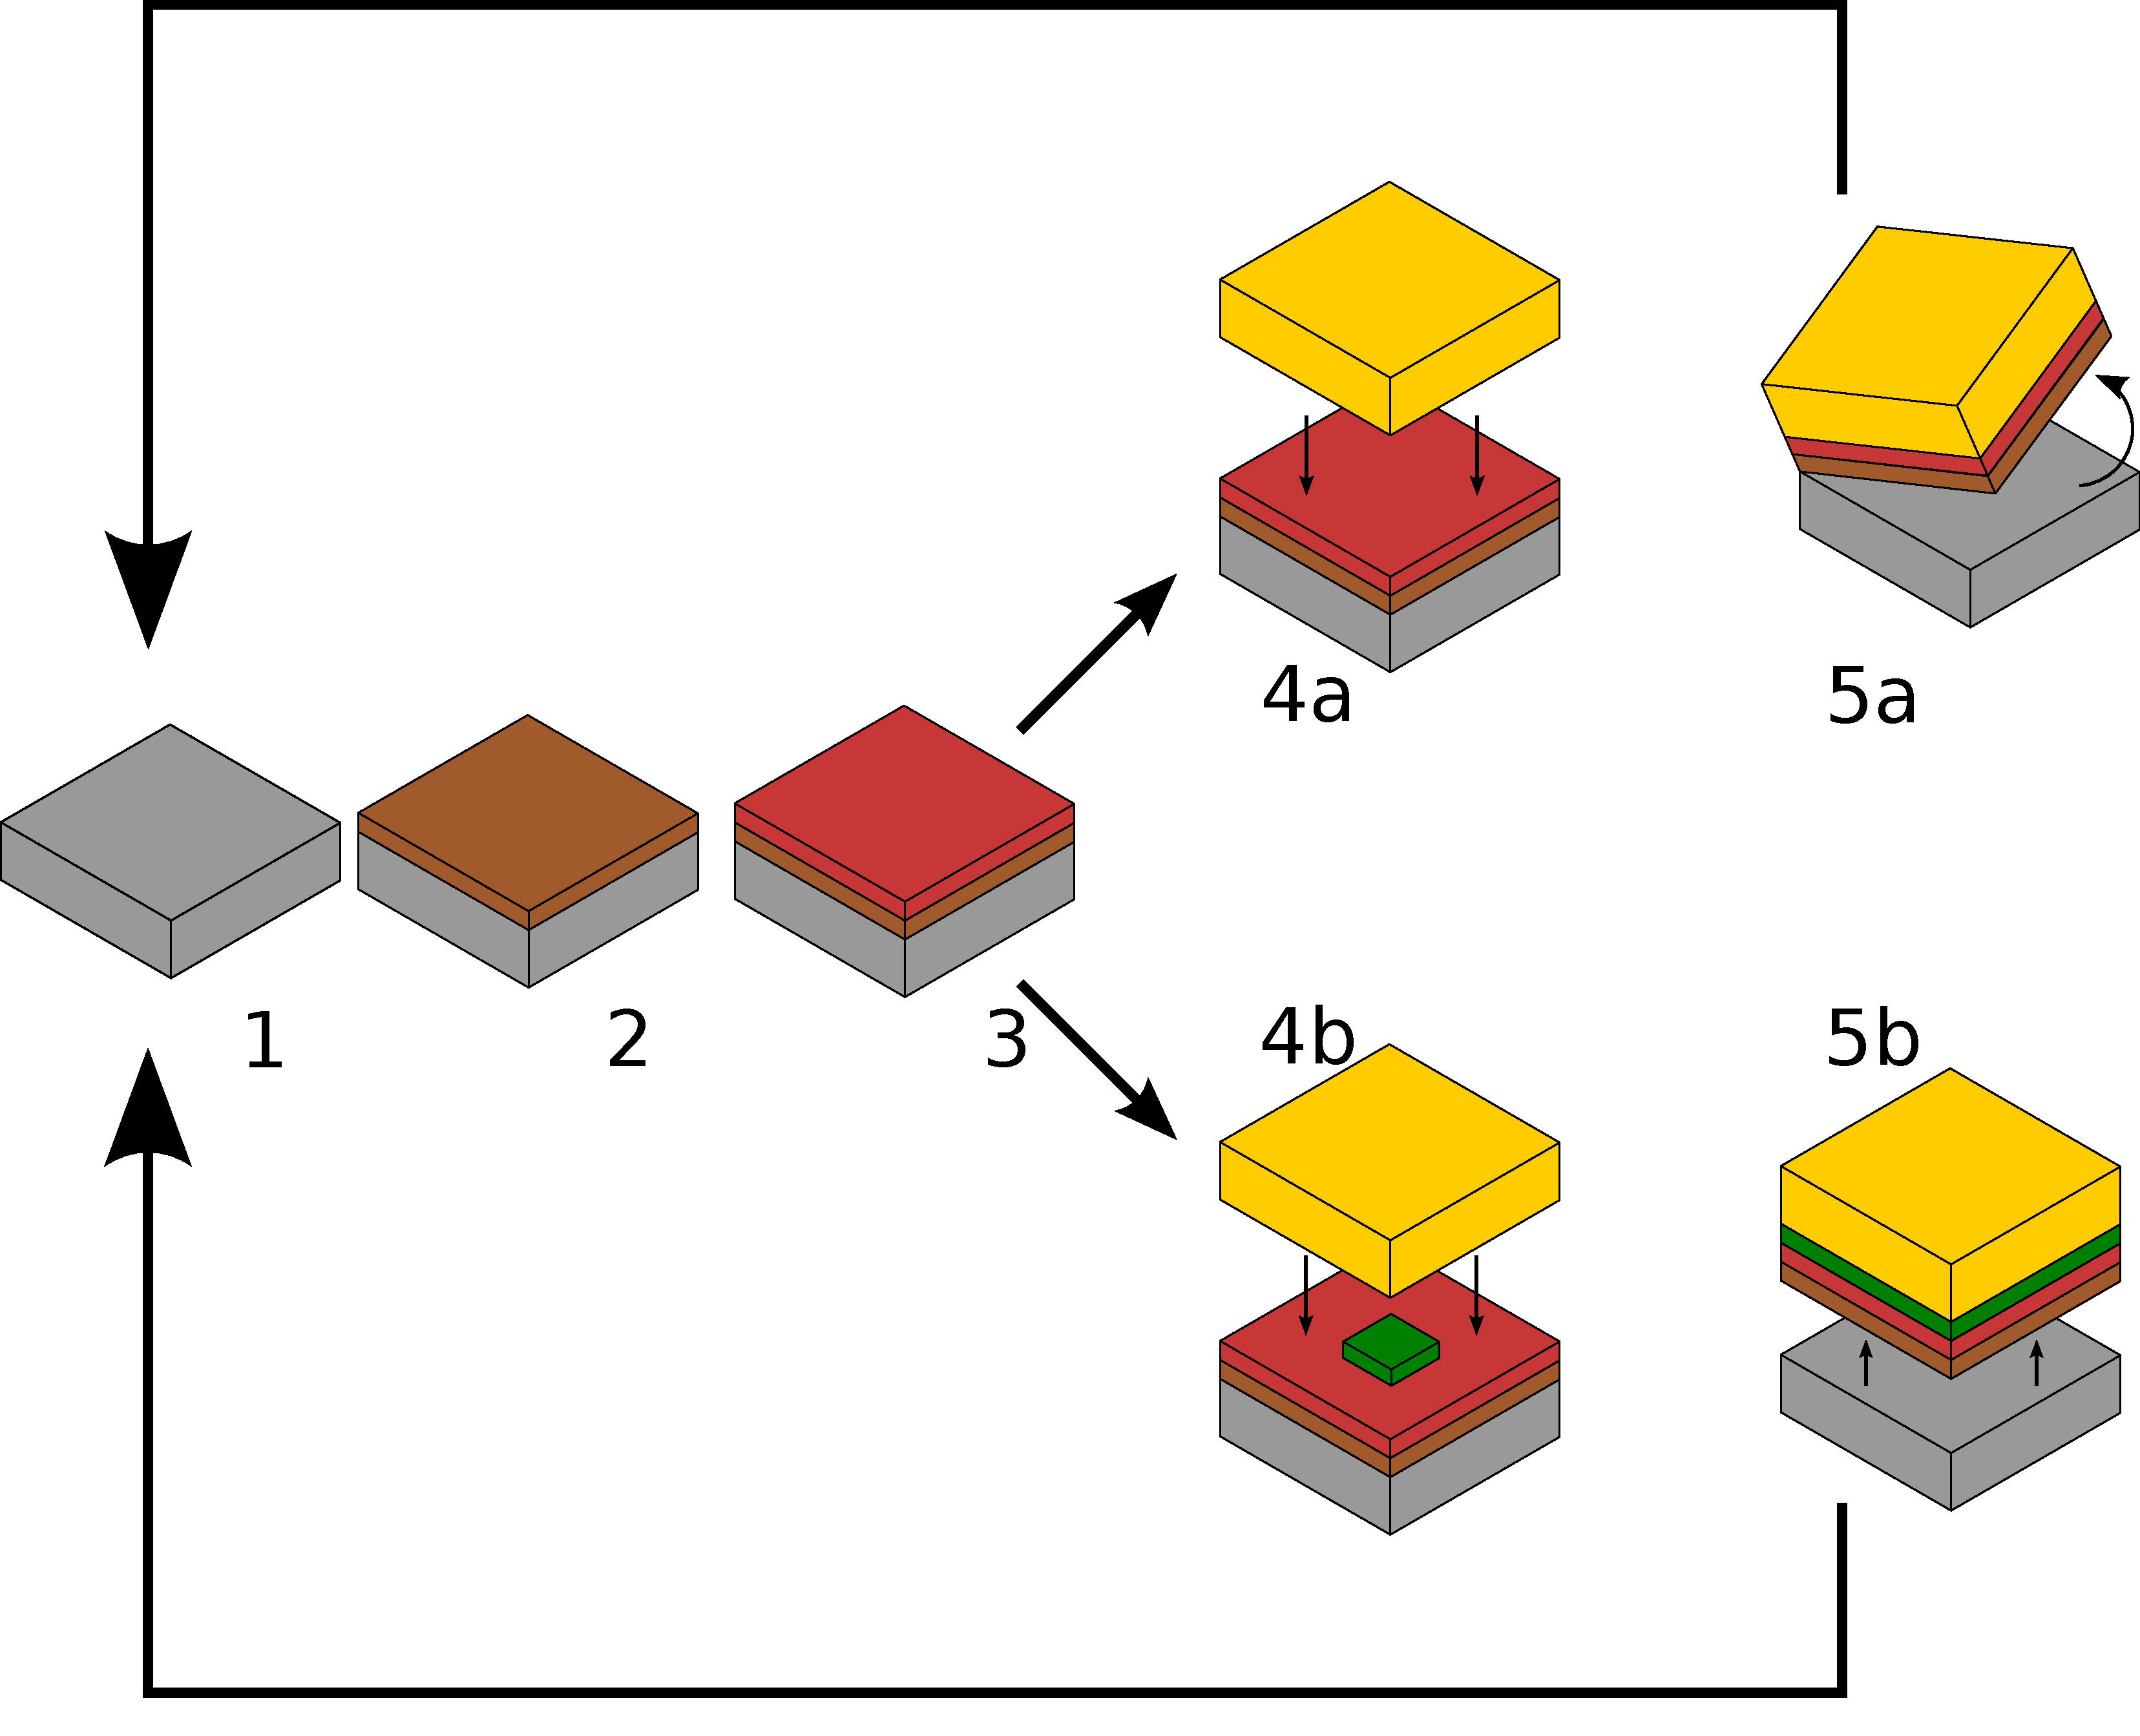
\includegraphics[width=\textwidth]{cdteliftoff_process}
    \caption{\label{fig:cdteliftoff_process}The generalized CdTe liftoff process}
\end{figure}
The flexible non-conductive liftoff carriers offered a first step to producing 
freestanding thin films, but electrical contact to the films is a key property in order 
to yield devices. To this end, thin films were coated with metal, first platinum (a known 
CdTe contact material) and then copper, in order to create a temperature stable surface. 
Samples were then wetted with solder paste and placed metal side down onto a copper 
surface, and thermally cycled through a solder reflow curve, as shown in 
\cref{fig:cdteliftoff_process}b. Upon removal from the oven, the films were found to have bonded to the copper surface and spontaneously lifted off from the original sapphire substrate. These experiments have demonstrated that the production of freestanding thin films by the liftoff phenomon is remarkably simple and straightforward.

Concurrent to investigations into the production of freestanding thin films via the liftoff process, the obvious question arose as to the properties of these films when compared to those attached to the epitaxial substrate. 2DXRD measurements were undertaken on thin films before, \cref{fig:cdteliftoff_F22_attached} and after \cref{fig:cdteliftoff_F22_released}, liftoff processing using two part epoxy.
\begin{figure}
    \centering
    \begin{subfigure}[b]{0.4\textwidth}
        \centering
        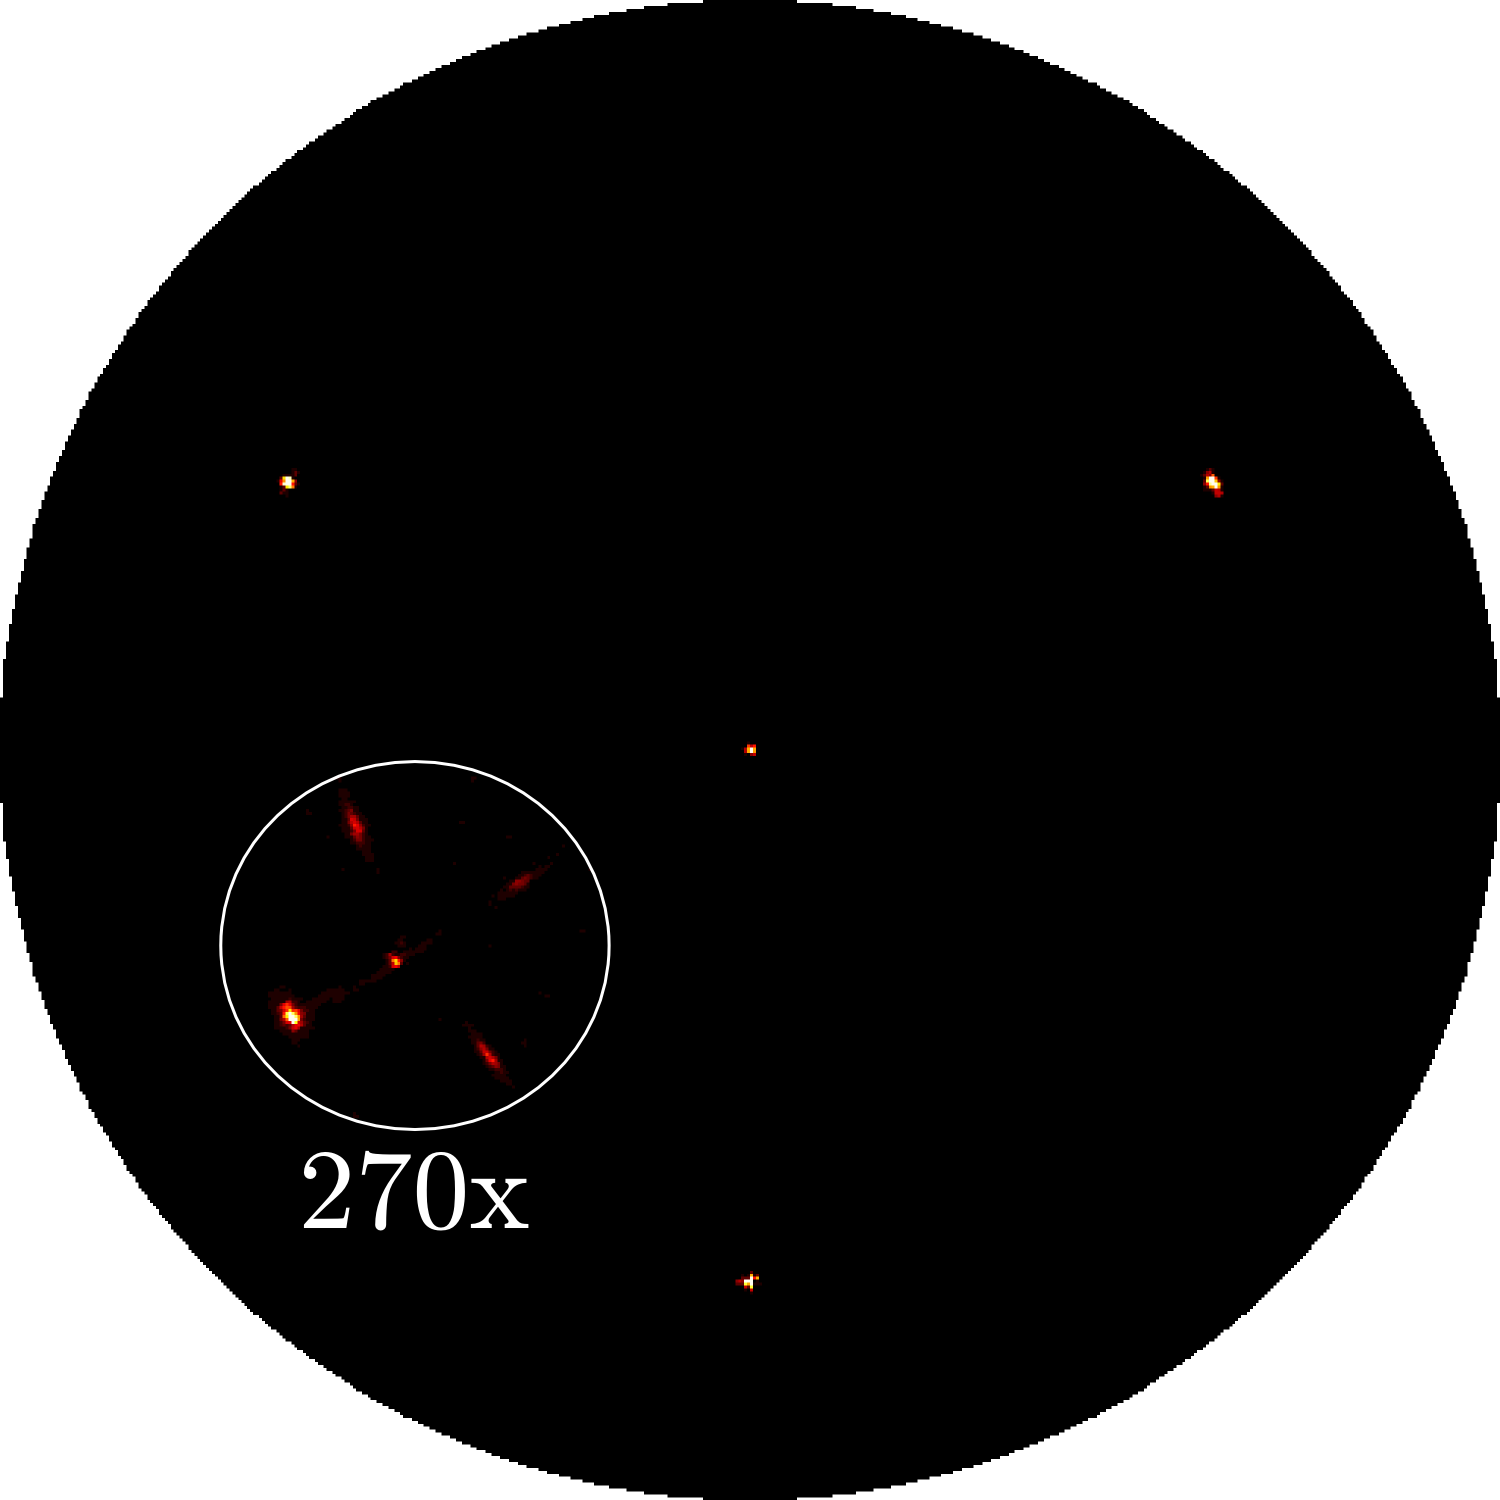
\includegraphics[width=\textwidth]{cdteliftoff_F22_attached}
        \caption{\label{fig:cdteliftoff_F22_attached}(111) Pole figure of as-grown CdTe on sapphire}
    \end{subfigure} %
    \begin{subfigure}[b]{0.4\textwidth}
        \centering
        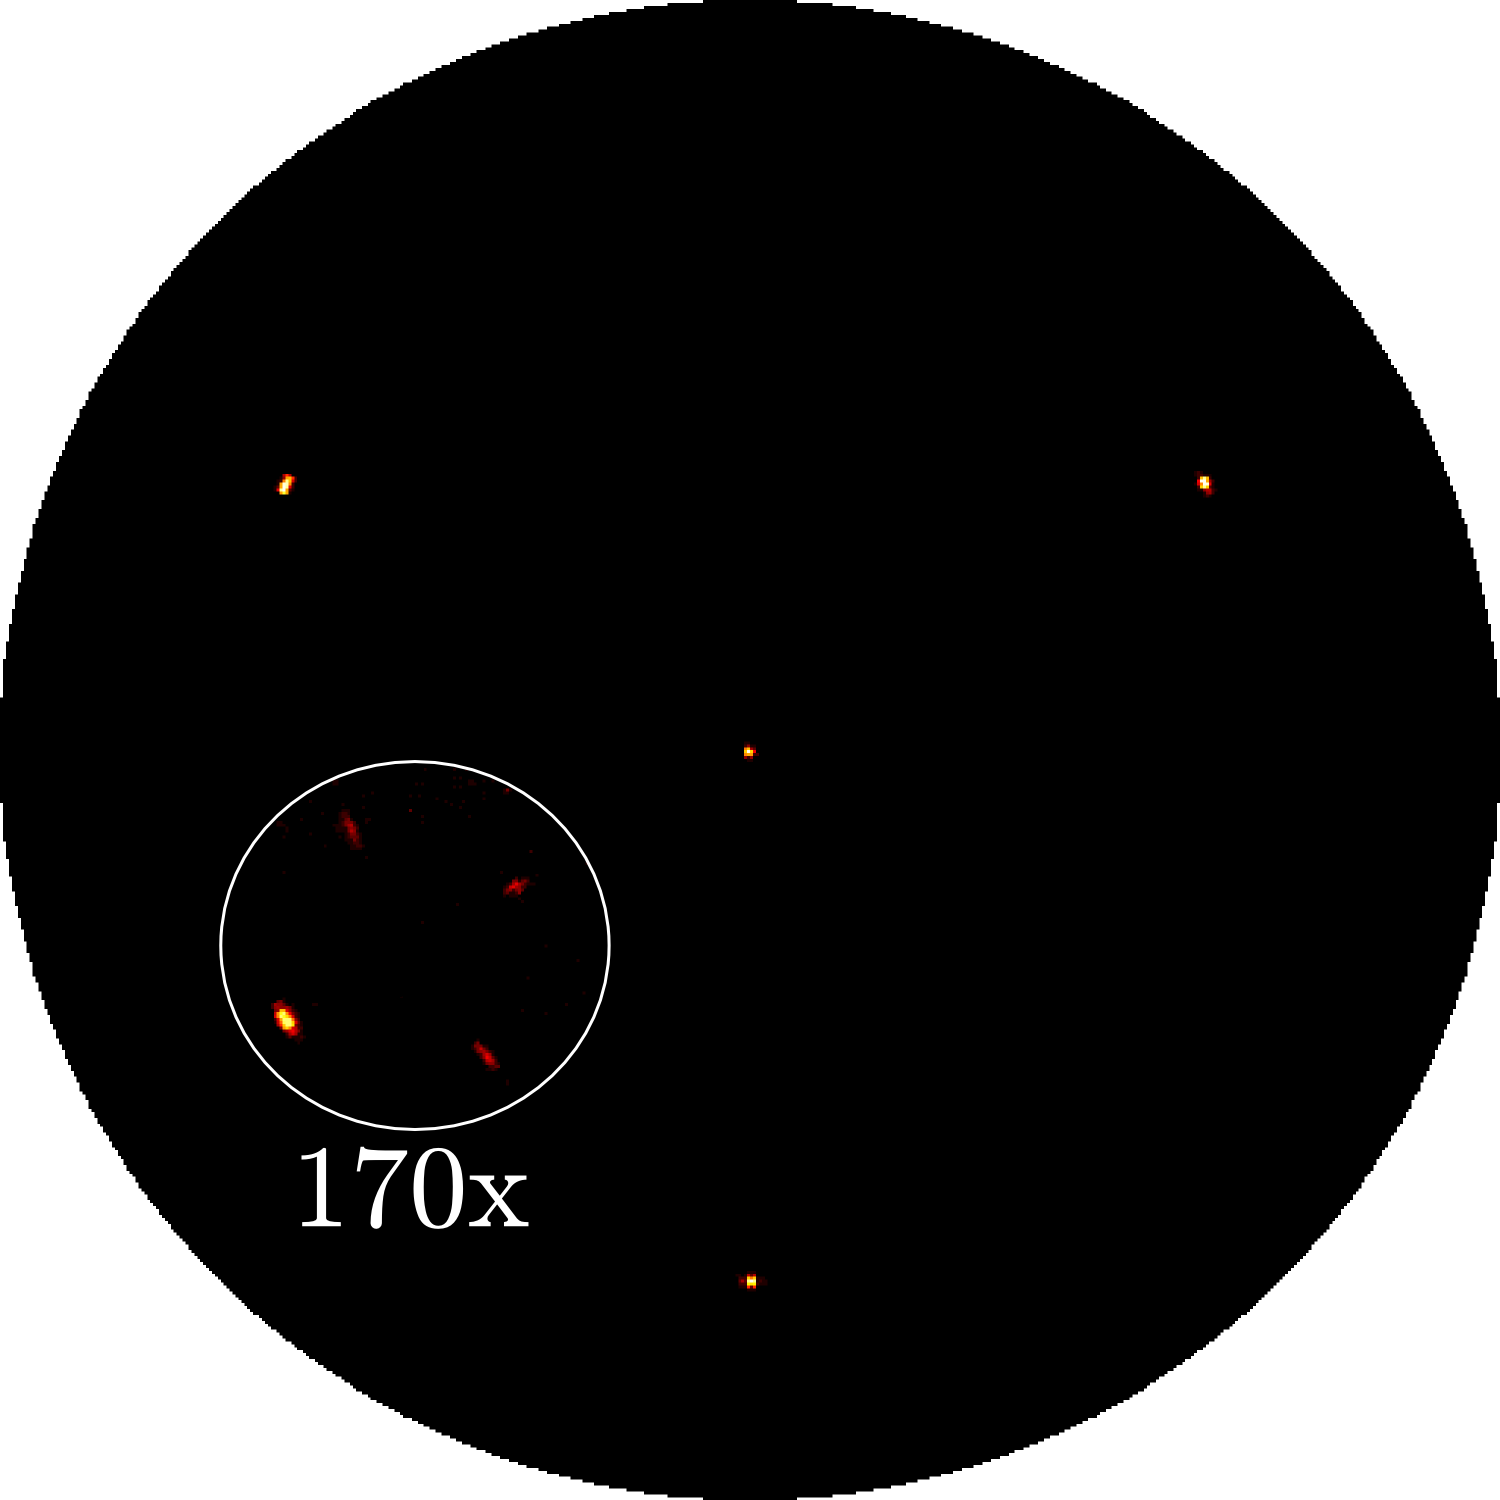
\includegraphics[width=\textwidth]{cdteliftoff_F22_released}
        \caption{\label{fig:cdteliftoff_F22_released}2DXRD of single crysal CdTe thin film on epoxy carrier}
    \end{subfigure}
    \caption{\label{fig:cdteliftoff_2DXRD}Attached and released CdTe pole figures}
\end{figure}



\section{Implications for Symmetry and Energy at Epitaxial Surfaces}

\chapter{CdTe Growth on Reconstructed \texorpdfstring{SrTiO$_3$}{SrTiO3}}
\section{Introduction}
As part of the ongoing research into the growth of CdTe, various other oxide single crystals were examined for possible use as substrates. One of those substrates, SrTiO\textsubscript{3}, while it did not ultimately yield particularly high quality CdTe, did provide some interesting insights into the potential for surface reconstructions to play a role in epitaxy.

The role of both substrate offcut and high temperature surface reconstructions were examined through the growth of CdTe on as-received and reconstructed SrTiO\textsubscript{3} substrates. This work was done in close collaboration with Dr. Robert Hughes and Dr. Svetlana Neretina and was published in Applied Surface Science\cite{Neretina2009a}.
\section{Experimental}
CdTe films were deposited on both the as-received and
reconstructed surface of (100) SrTiO\textsubscript{3} (MTI Corporation). Step-
terrace formation relied upon the miscut originating from the
inaccuracies in the crystallographic alignment carried out prior to
the cutting and polishing of the substrates (manufacturer’s miscut
tolerance 0.5\degree). As a result, the degree of miscut could only be
varied through the use of substrates from different batches. Due to
the high temperatures required, the surface reconstruction took
place ex situ in a quartz tube furnace. Prior to annealing, the
substrates were etched in BHF for 90~s. Anneals were conducted in
flowing oxygen (60 SCCM) at 1000\celsius{} for 10~h. \cref{fig:srtio3_sub_afm} shows
atomic force microscopy (AFM) images for the as-received and
surface reconstructed substrates relevant to this work. As
expected, only the annealed substrates exhibit the step-terrace
structure with unit cell step heights. The difference in terrace
width for the surfaces shown in \cref{fig:srtio3_sub_afm}b and c can be attributed to a
miscut difference estimated at 0.358\degree. Also present on each image
are the crystallographic axes obtained through X-ray diffraction
(XRD). Note that a nearly identical in-plane step direction exists for
both reconstructed surfaces. As this direction is close to, but not
aligned with the [011] axis of SrTiO\textsubscript{3}, it is expected that the steps
exhibit a sawtooth morphology, but on length scales not readily
observed using atomic force microscopy.
\begin{figure}
    \centering
    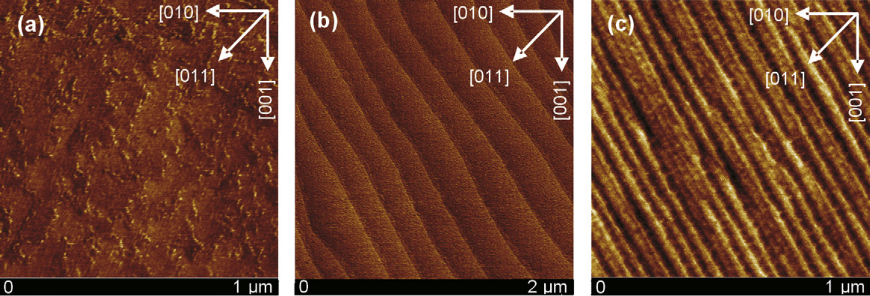
\includegraphics[width=\textwidth]{srtio3_sub_afm}
    \caption[AFM of SrTiO\textsubscript{3} surfaces]{\label{fig:srtio3_sub_afm}AFM images for the (a) as-received (100) SrTiO\textsubscript{3} substrate, (b) a reconstructed surface with an average terrace width of approximately 200 nm and (c) a reconstructed surface with a terrace width of approximately 50 nm. From the step heights and terrace widths it is estimated that the miscuts for the two reconstructed surfaces are (b) 0.118\degree{}
        and (c) 0.468\degree{}.}
\end{figure}

CdTe films were deposited on the three SrTiO\textsubscript{3} surfaces shown
in \cref{fig:srtio3_sub_afm} using pulsed laser deposition. A deposition rate of 20 nm/min was achieved by
operating the laser at a repetition rate of 10~Hz with a substrate to
target distance of 3.5~cm. Films were grown to
a thickness of 300~nm as determined using a spectroscopic variable
angle ellipsometer (Horiba Jobin Yvon, France). Morphological and
structural characterization was then conducted on the films
produced using AFM and 2DXRD.
\section{Results and Discussion}
\cref{fig:srtio3_pole} shows the (111) CdTe pole figures for the three substrates
shown in \cref{fig:srtio3_sub_afm}. The dramatic differences observed between films
deposited on the as-received and annealed substrates indicate that
the surface reconstruction gives rise to a complete re-alignment of
the CdTe grains. The pole figure for the as-received surface is
consistent with a [111] oriented film. The fact that twelve peaks
exist in the outer ring, instead of the three expected for a single
crystal, indicates that there are four in-plane grain orientations.
The pole figures for the films deposited on the surface reconstructed substrates show that both films are predominantly [211]
oriented. The twelve peaks in the central ring and twenty-four
peaks in the outer ring denote twelve in-plane grain orientations. Each peak in the central ring comes from a different grain, the intensity differences indicate that some grains form
preferentially over others. Note that of the twelve peaks both
the strongest and weakest is in-line with the miscut direction for
both of the reconstructed surfaces and that the degree of this
preferential orientation is stronger for the reconstructed surface
having the narrow terrace width. An examination of the low
intensity pole figure peaks (not visible in the figures), indicates that
some [111] CdTe grains exist in these nominally [211] films, but
at the 10\% level. While these [111] grains contribute to
the intensity at the centre of the pole, the response there is almost
entirely due to the (100) SrTiO\textsubscript{3} substrate.
\begin{figure}
    \centering
    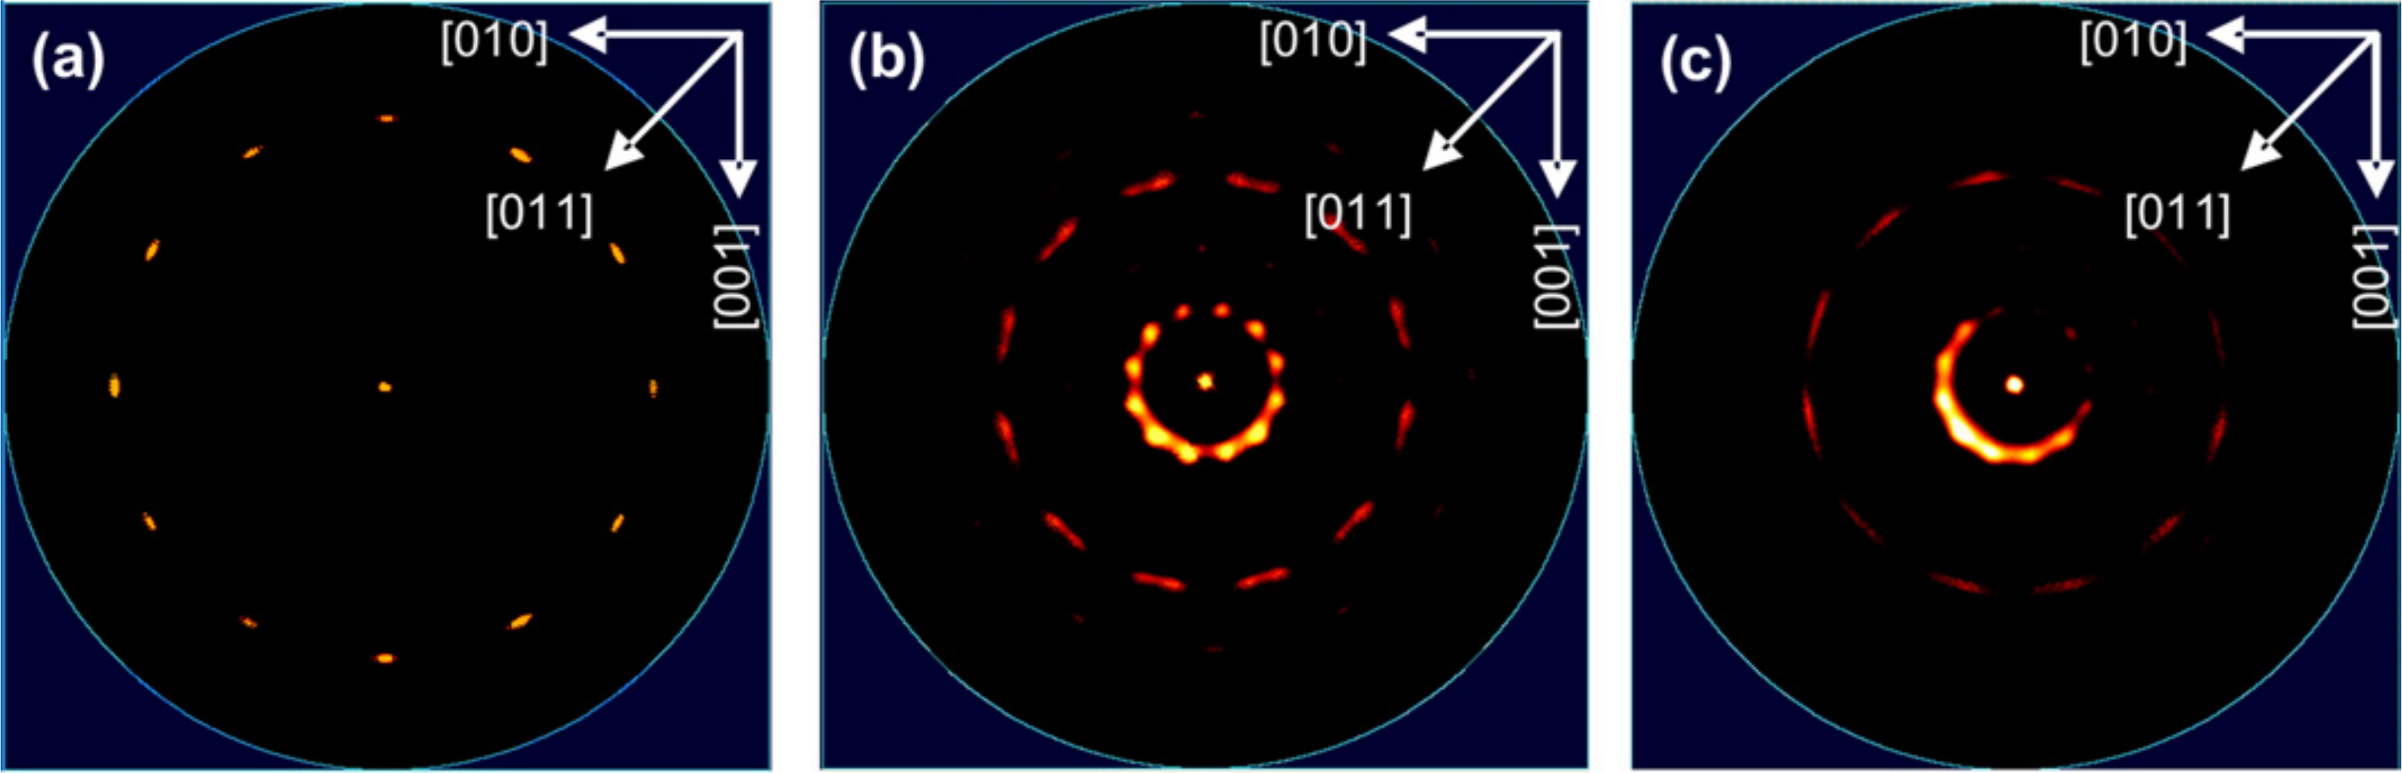
\includegraphics[width=\textwidth]{srtio3_pole}
    \caption[Pole figures of CdTe grown on SrTiO\textsubscript{3}]{\label{fig:srtio3_pole}(111) CdTe pole figures for films deposited on (a) the as-received (100) SrTiO\textsubscript{3} substrate (b) the reconstructed surface with wide terraces and (c) the reconstructed surface with narrow terraces. Indicated on each image are the substrate’s in-plane crystallographic axes obtained from XRD measurements.}
\end{figure}
\begin{figure}
    \centering
    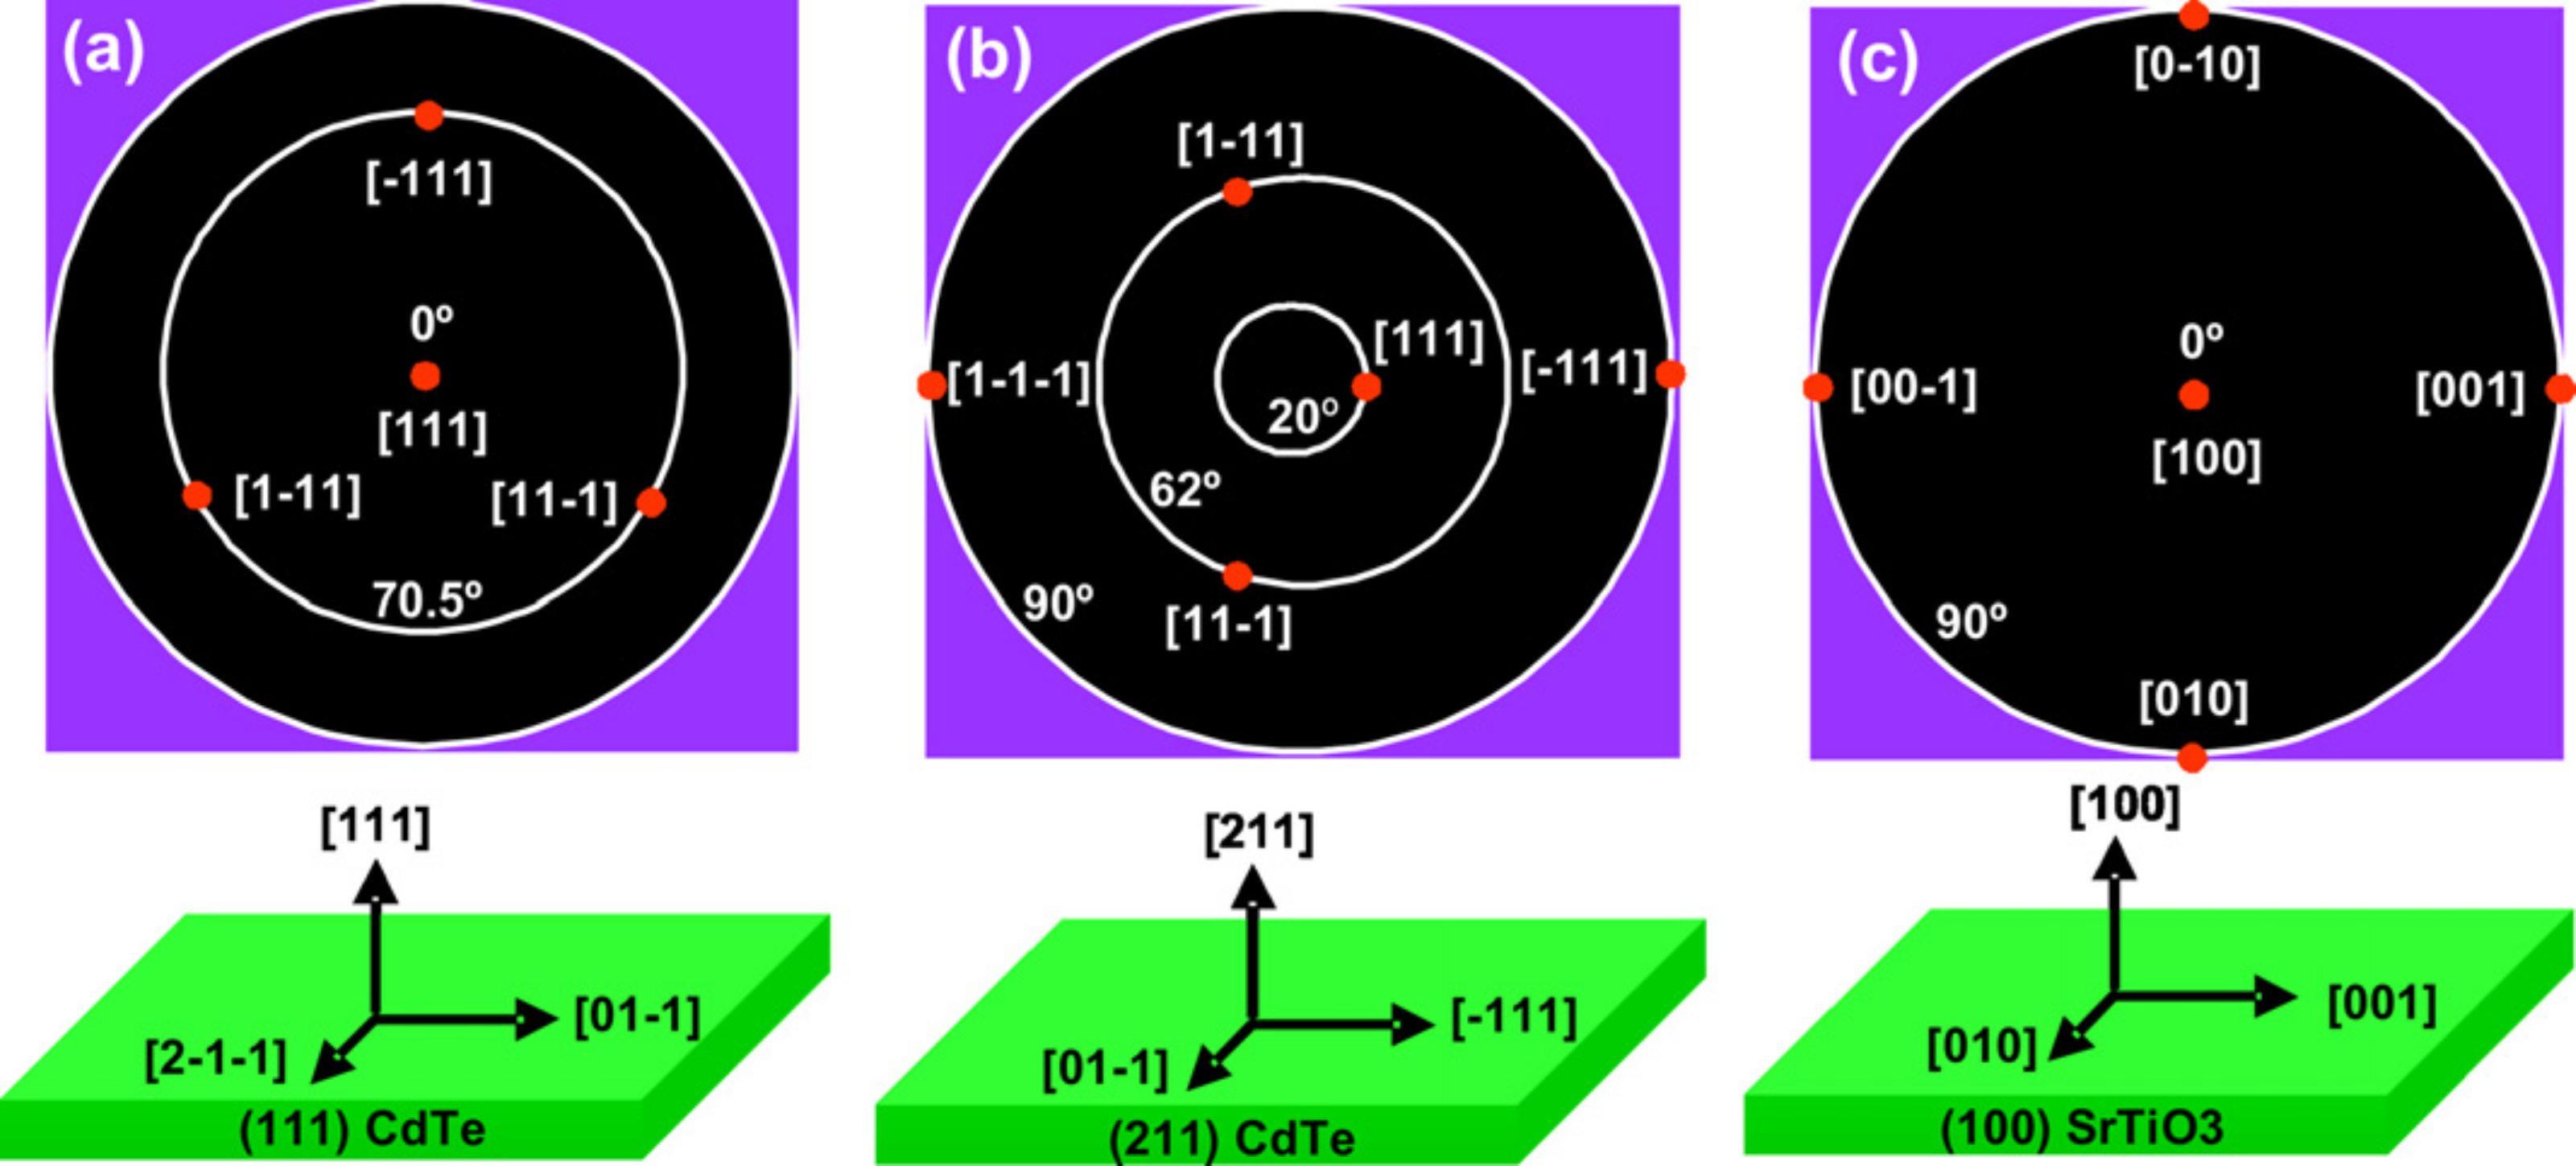
\includegraphics[width=\textwidth]{srtio3_sim_pole}
    \caption{\label{fig:srtio3_sim_pole}Schematics showing the (111) pole figure expected for a single crystal CdTe film with a a) [111] and b) [211] orientation. c) Schematic showing the (100) pole figure expected for a [100] oriented SrTiO\textsubscript{3} substrate. The surface normal and in-plane Miller indicies are also shown for each case.}
\end{figure}

Grain formation for a given film/substrate combination is
determined by the interface energy. For the case of the as-received
(100) SrTiO\textsubscript{3} substrate the interface energy is minimized through
the formation of [111] CdTe grains. This interfacial relationship is
not surprising as CdTe has demonstrated a high propensity for
forming it almost irrespective of the substrate surface offered\cite{Neretina2006}.
The resulting interface, however, must overcome the seemingly
incompatible situation brought about when the four-fold symmetric substrate surface mates with the six-fold symmetric (111)
plane of CdTe. In this scenario it is reasonable to expect that the
resulting in-plane grain structure reflects both a suitable fit to the
substrate’s atomic arrangement as well as its underlying symmetry. The (111) pole figure results indicate that this is indeed the
case as there exists a four-fold symmetric grain structure which is
commensurate with the substrate’s cubic crystal structure. The
XRD data indicates that these grains are oriented as shown
schematically in \cref{fig:srtio3_tri_on_100}a. The triangles symbolize the orientation of
the (111) planes on the surface of SrTiO\textsubscript{3} represented by the
dotted pattern. The arrows on the triangles denote the three
equivalent (111) CdTe planes that project out of its surface. Note
that each of these four triangles match poorly to the substrate’s
lattice constant in all but one direction. In this direction, it is nearly
equal to two of the substrate’s unit cells (mismatch = 1.6\%). This
one-dimensional match is preferred to such extents that only
grains that comply with it exist within the film. To appreciate the
uniqueness of the four grains it should be noted that, for the arrows
denoting the (111) equivalent planes, no two arrows point in the
same direction. It is these directions that give rise to the twelve
peaks in the outer ring of the (111) pole figure as is evident from
\cref{fig:srtio3_tri_on_100}b.
\begin{figure}
    \centering
    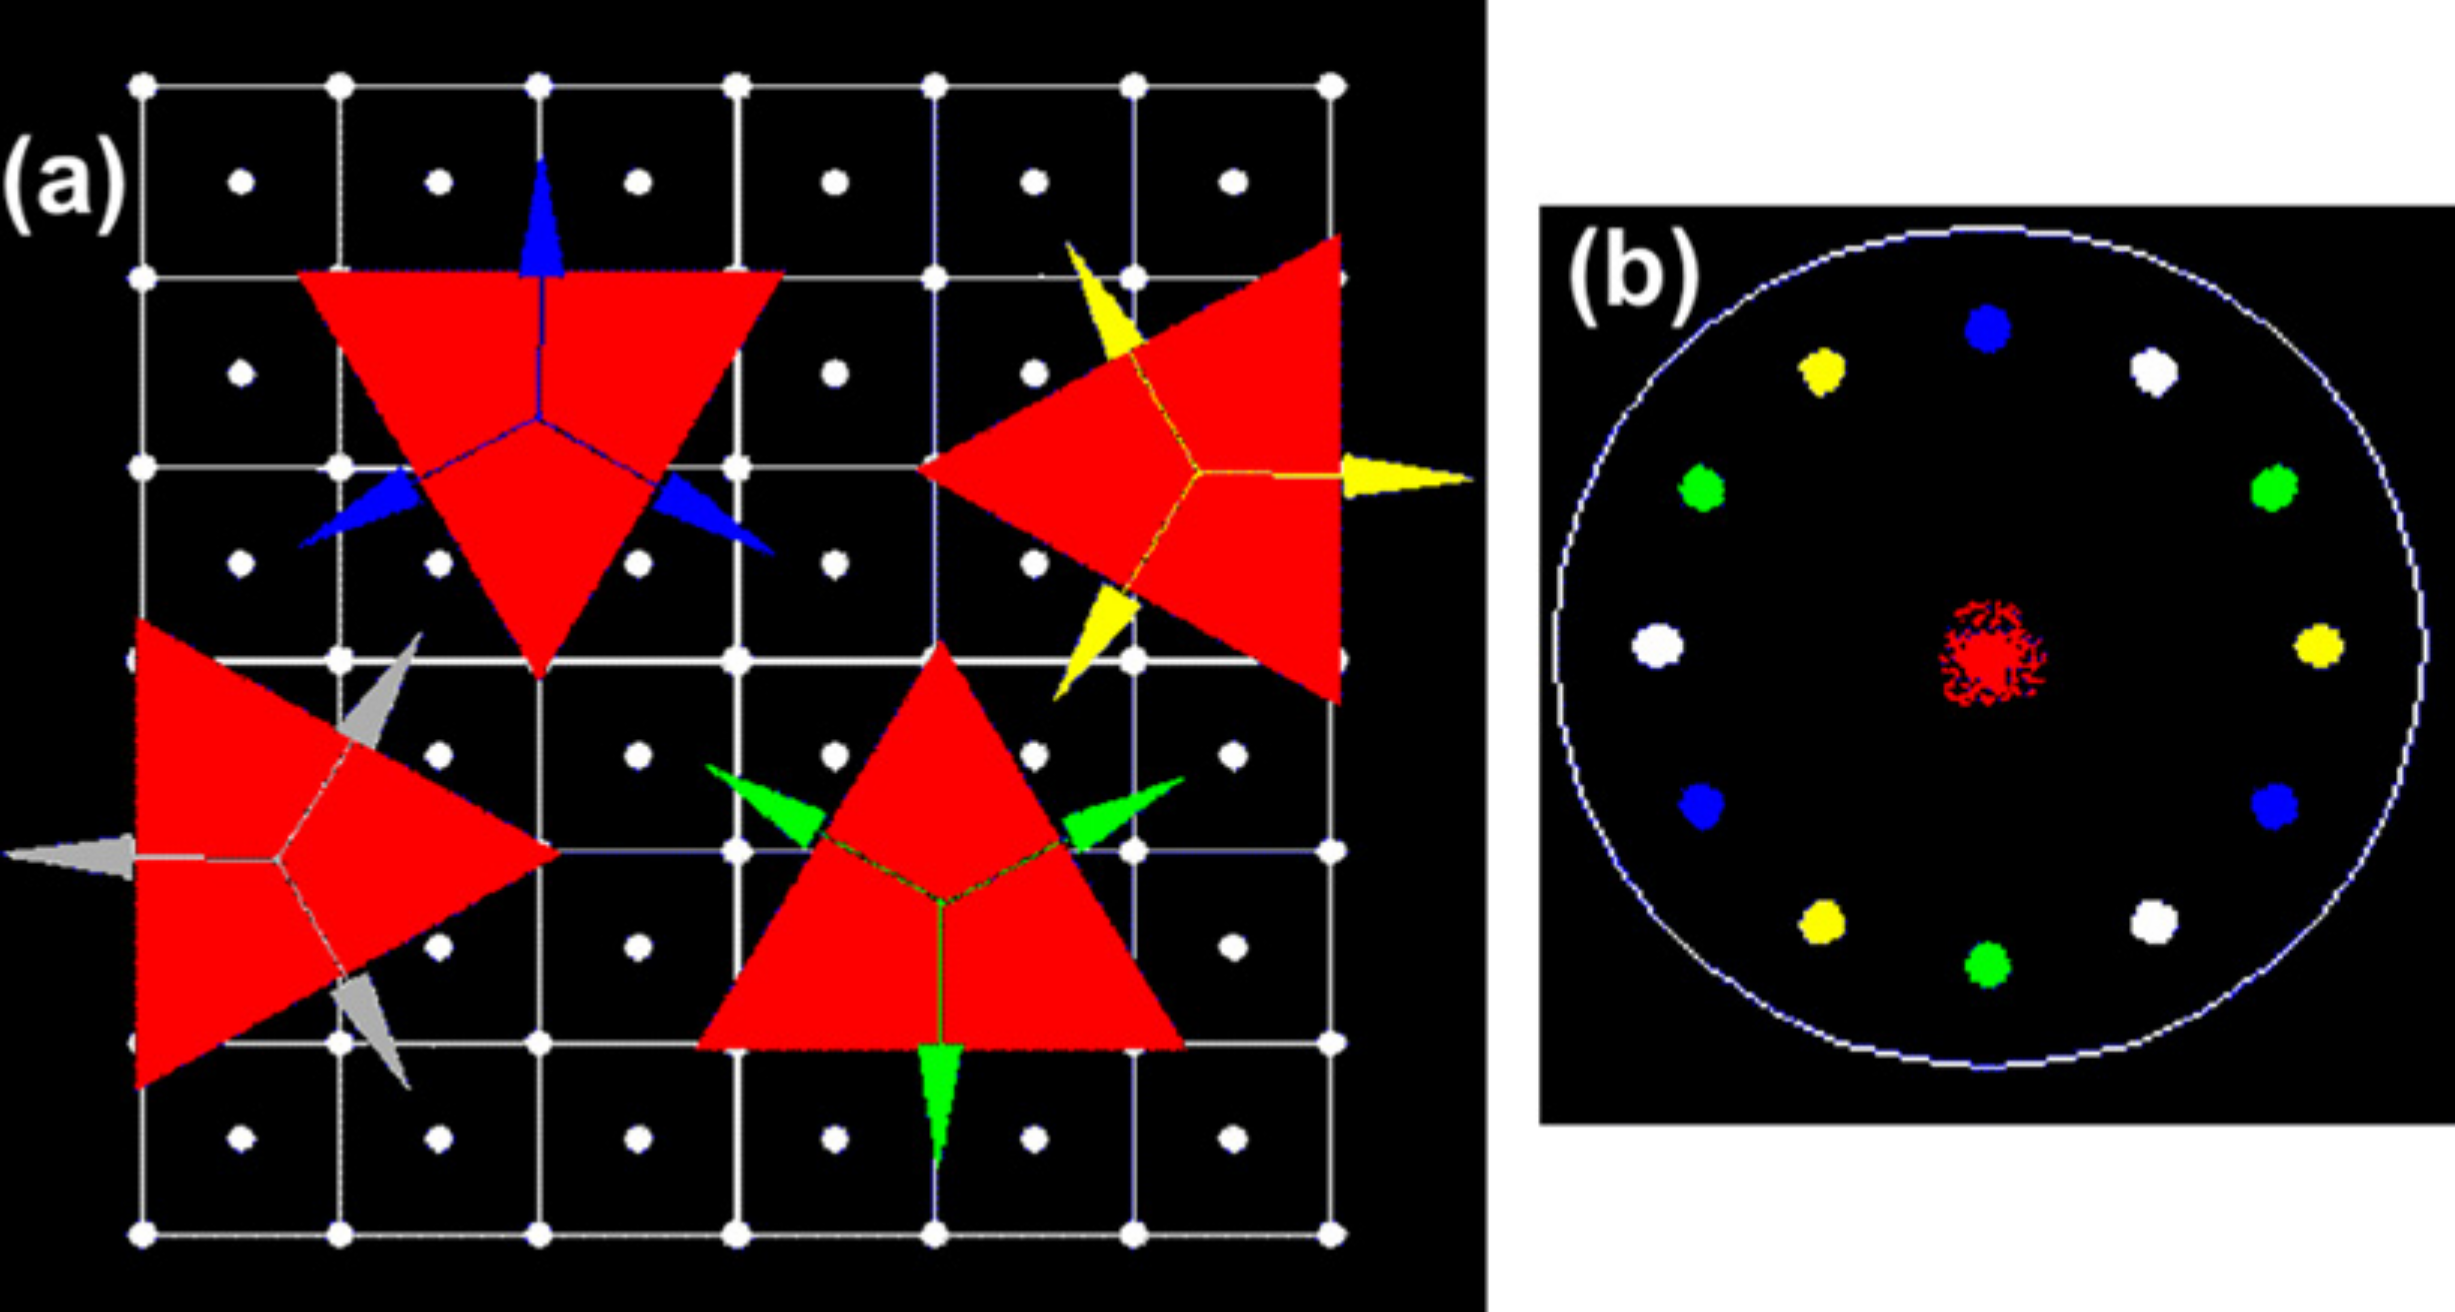
\includegraphics{srtio3_tri_on_100}
    \caption[CdTe grains on (100) SrTiO\textsubscript{3}]{\label{fig:srtio3_tri_on_100}a) Schematic illustrating the four possible [111] CdTe grain orientations (triangles) for films deposited on the SrTiO\textsubscript{3} substrate (dotted background). The arrows on
        each triangle denote the direction of the three equivalent (111) planes that emerge from the surface. Note that no two arrows are pointing in the same direction. For each
        grain orientation there exists a one-dimensional geometrical fit (mismatch = 1.6\%) to the substrate in either the vertical or horizontal directions. b) Schematic showing the
        resulting (111) pole figure obtained from the four grains where the colour of the dot on the pole figure corresponds to the grain from which it was derived.}
\end{figure}
\begin{figure}
    \centering
    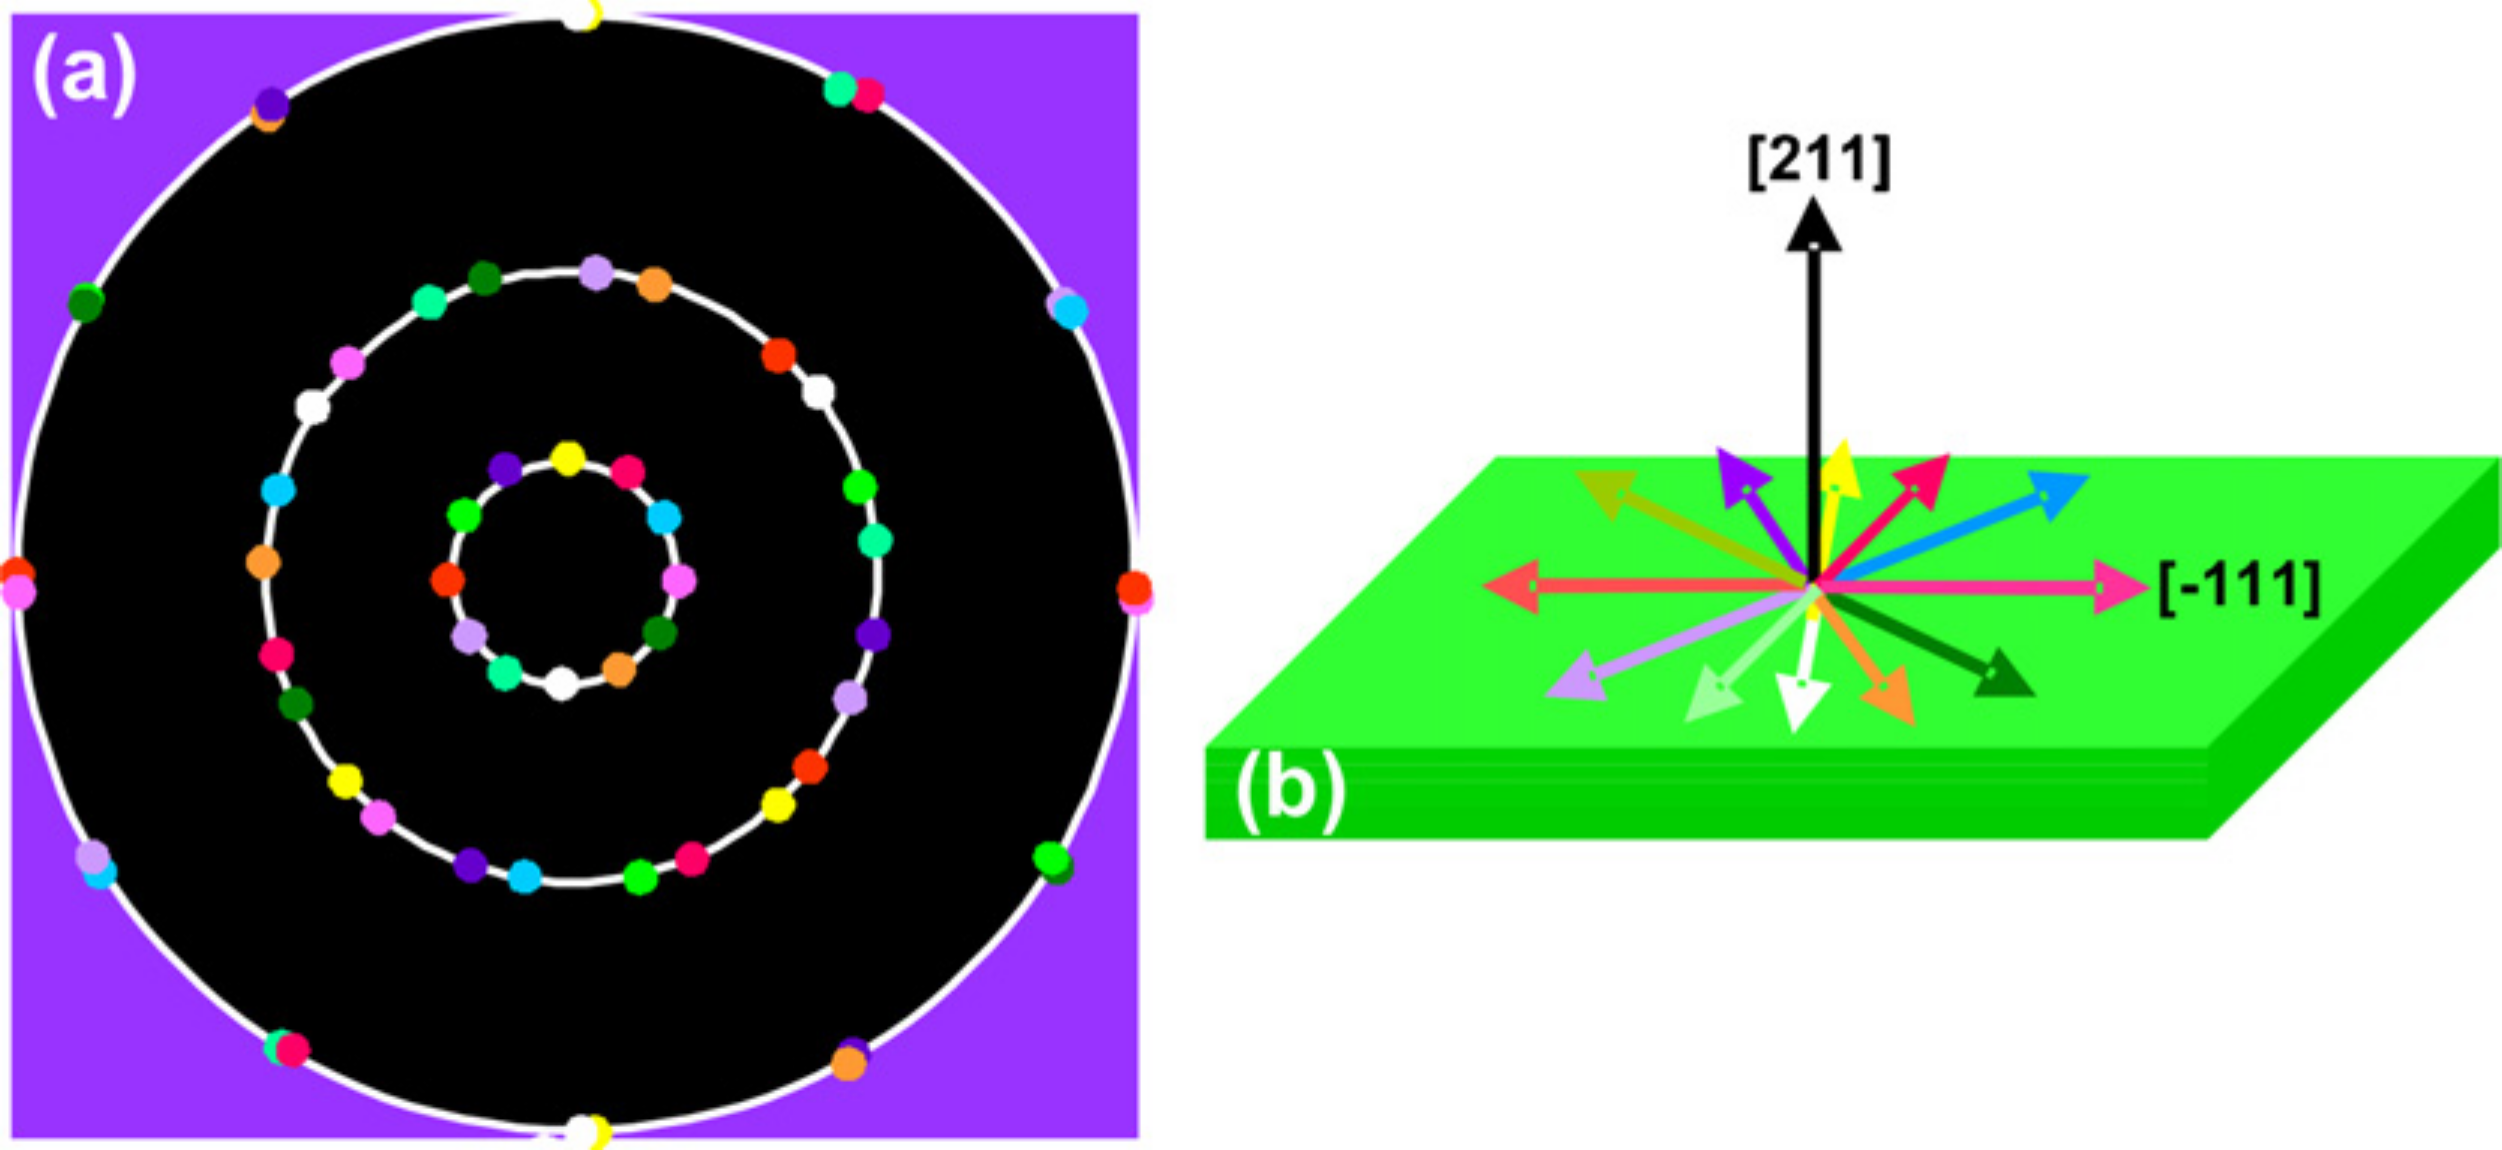
\includegraphics{srtio3_211_sim_polefigure}
    \caption[Simulated pole figure of CdTe on reconstructed SrTiO\textsubscript{3}]{\label{fig:srtio3_211_sim_polefigure}a) Schematic detailing the twelve-fold symmetric [211] CdTe grain structure observed for films deposited on the surface reconstructed substrates. The contribution
        from each grain is denoted by a different colour. Note that the pattern corresponding to a single crystal [211] CdTe film (\cref{fig:srtio3_sim_pole}b) is repeated twelve times. b) Schematic showing the in-plane [$\overline{1}$11] direction for each of the [211] grains.}
\end{figure}

The formation of a [211] CdTe film on a surface reconstructed
(100) SrTiO\textsubscript{3} substrate was quite unexpected. CdTe films with this
orientation have been deposited, but only when the interface
energy is minimized through the use of [211] oriented substrates
\cite{Lange1991b,Million1996,Rujirawat1997a,Zanatta1998}. While [211] substrates provide an appropriate template
for [211] growth, there exist no obvious symmetry arguments
that would allow for twelve symmetrically distributed grains to be
accommodated on the bulk surface of (100) SrTiO\textsubscript{3}. Instead, it is
expected that the origin of the [211] CdTe grains lies with the
epitaxial relationship formed between the (211) planes and the
surface reconstruction. In this case, it is expected that the twelve-fold symmetric grain structure is commensurate with the underlying symmetry of the substrate’s surface reconstruction. Thus,
insight into the nature of the reconstruction is obtained from the
observed grain structure. \Cref{fig:srtio3_211_sim_polefigure} shows a schematic representation
of the (111) CdTe pole figure where the contributions from each
grain are shown. The pole figure’s inner ring demonstrates a
twelve-fold symmetry in the grain structure as it is comprised of twelve nearly equally spaced peaks where each peak originates
from a different grain orientation. Also of significance is the fact
that the wide terrace widths shown in \cref{fig:srtio3_sub_afm}b give rise to [211]
CdTe grains even though the film grain size is often smaller than
the width of the terrace. Thus, it appears that [211] grain
formation does not rely on nucleation at the substrate steps. This is
a strong indication that the atomic scale surface reconstruction is a
dominant factor in the promotion of the [211] grains.

Of the three surface reconstructions known to form in an
oxygen ambient, only the c($4\times2$) and c($6\times2$) reconstructions
present a surface structure where there exist reasonable symmetry
arguments able to account for the formation of a [211] CdTe film
having a twelve-fold symmetric grain structure. Such a grain
structure must arise from the symmetries of the underlying
substrate as it provides the only means for the isolated grains to
establish a symmetrical arrangement when first formed in an
island growth mode. The (211) plane of CdTe, shown in \cref{fig:srtio3_cdte211}, is
one-fold symmetric and consists of a series of rows comprised of
alternating cadmium and tellurium atoms separated by distances of 8.49 or 2.83 \AA. \Cref{fig:srtio3_c4x2} shows a schematic of the c($4\times2$) TiO\textsubscript{2} surface reconstruction proposed by Castell\cite{Castell2002}. It consists of a
series of alternating rows of titanium and oxygen atoms. The top
layer has a TiO\textsubscript{2} stoichiometry, but it is sparsely populated with
only one quarter the number of atoms present in the TiO\textsubscript{2} layers
found in the bulk\cite{Castell2002}. With every second row of titanium atoms
offset relative to each other they align in a pseudo-six-fold
symmetric pattern. Possible geometric fits of the (211) CdTe plane
to this surface reconstruction are shown in \cref{fig:srtio3_c4x2}b. Each of the three
possible geometric fits shown would give rise to two unique grain
types due to the one-fold symmetry of the (211) plane. Six other
domain structures would also form by virtue of the fact that the
c($4\times2$) surface reconstruction has two possible domains rotated
90\degree~relative to each other\cite{Castell2002}. The domain structure that develops
on the reconstructed surface arises from the fact that the rows of
titanium atoms have an equal probability of forming along the
[010] or [001] directions. The net result would be a twelve-fold
symmetric [211] CdTe grain structure. The c($6\times2$) surface
reconstruction, proposed by Jiang and Zegenhagen\cite{Jiang1996}, is shown
schematically in \cref{fig:srtio3_cdte211}. It too is a sparsely populated surface that
has the potential to accommodate the (211) CdTe planes in select
directions (\cref{fig:srtio3_cdte211}b). Here, the four geometrical fits shown give rise
to eight unique grain types. In a manner analogous to the c($4\times2$)
reconstruction, the c($6\times2$) reconstruction also has a domain
structure that gives rise to an additional set of eight grains rotated
90\degree{} to the ones shown in the figure. An examination of these
additional grains, however, reveals that only four of them provide
unique solutions as the other four rotate into solutions offered by
the first domain. Thus, a twelve-fold ($8 + 8 \times 4 = 12$) symmetric
(211) CdTe grain structure is expected for this surface.
\begin{figure}
    \centering
    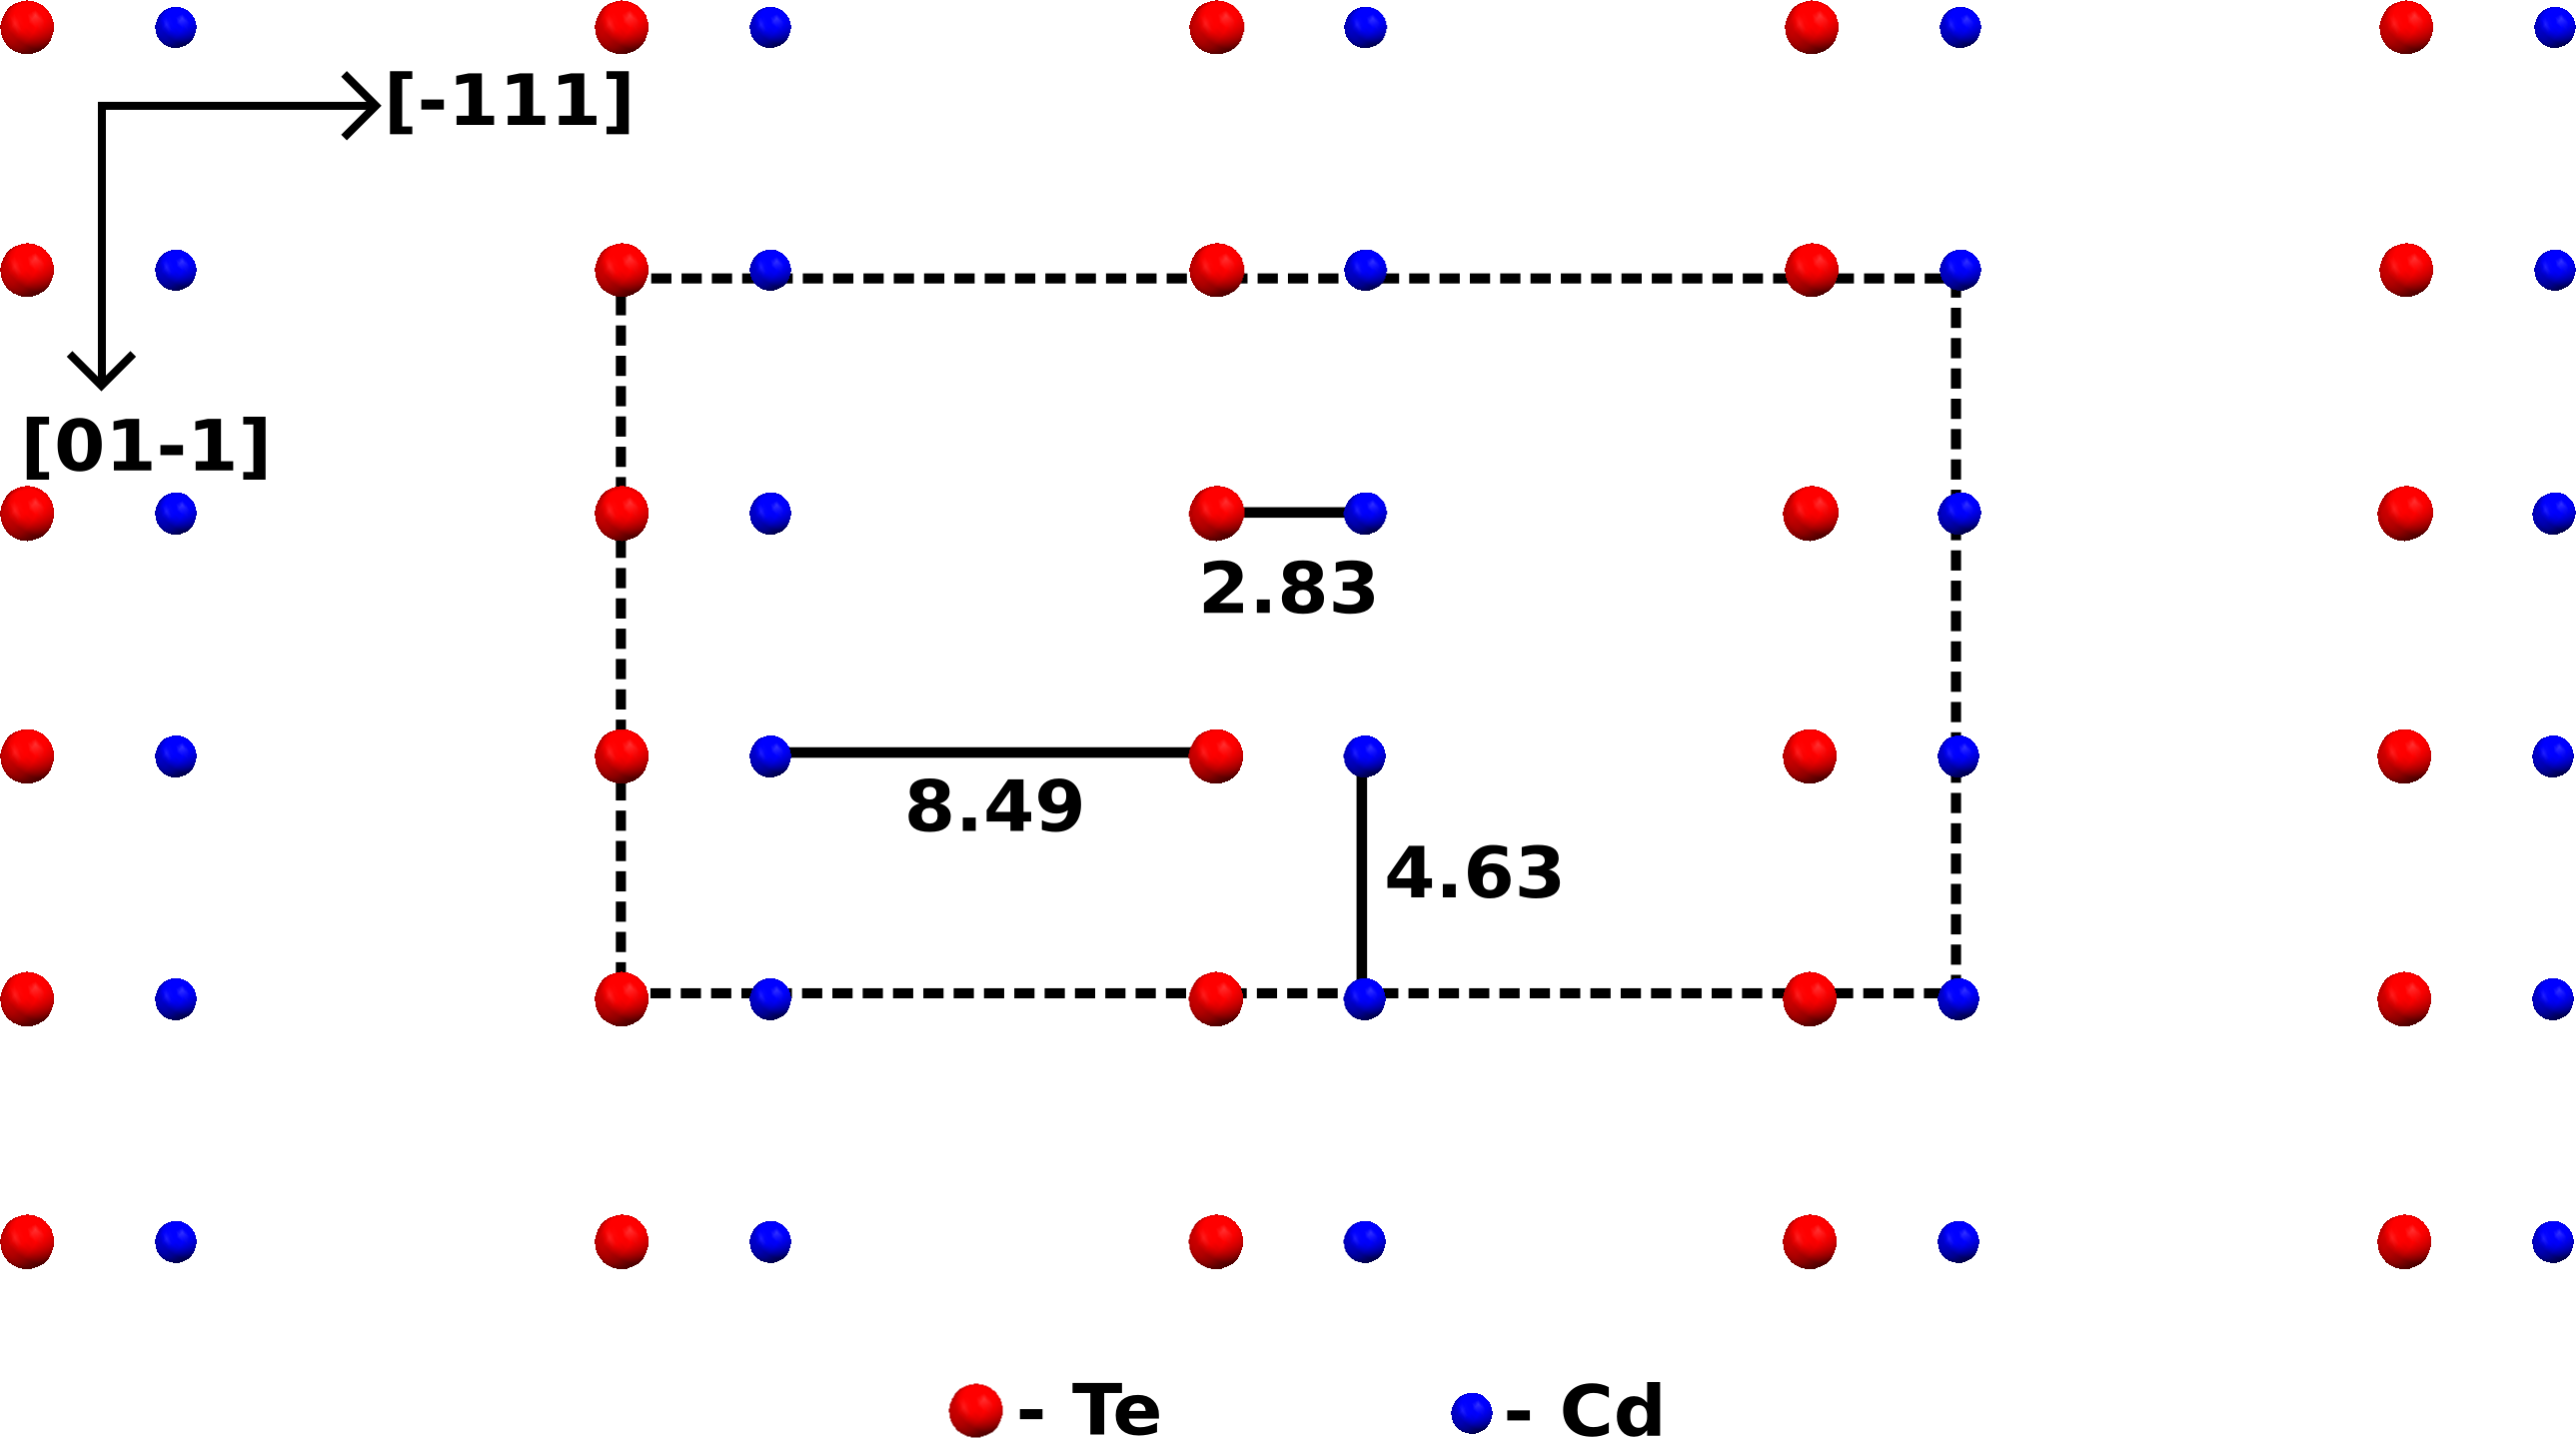
\includegraphics[width=0.8\textwidth]{srtio3_cdte211}
    \caption[Projection of (211) CdTe unit cell on SrTiO\textsubscript{3} surface]{\label{fig:srtio3_cdte211}Schematic of the (211) plane of CdTe with the interplanar dimensions
        labelled in units of angstroms. The area outlined by the dashed lines is used in
        subsequent figures to demonstrate how this structure fits to (100) SrTiO\textsubscript{3} surface
        reconstructions. The Miller indices shown correspond to the crystallographic
        orientation of the (211) CdTe plane.}
\end{figure}
\begin{figure}
    \centering
    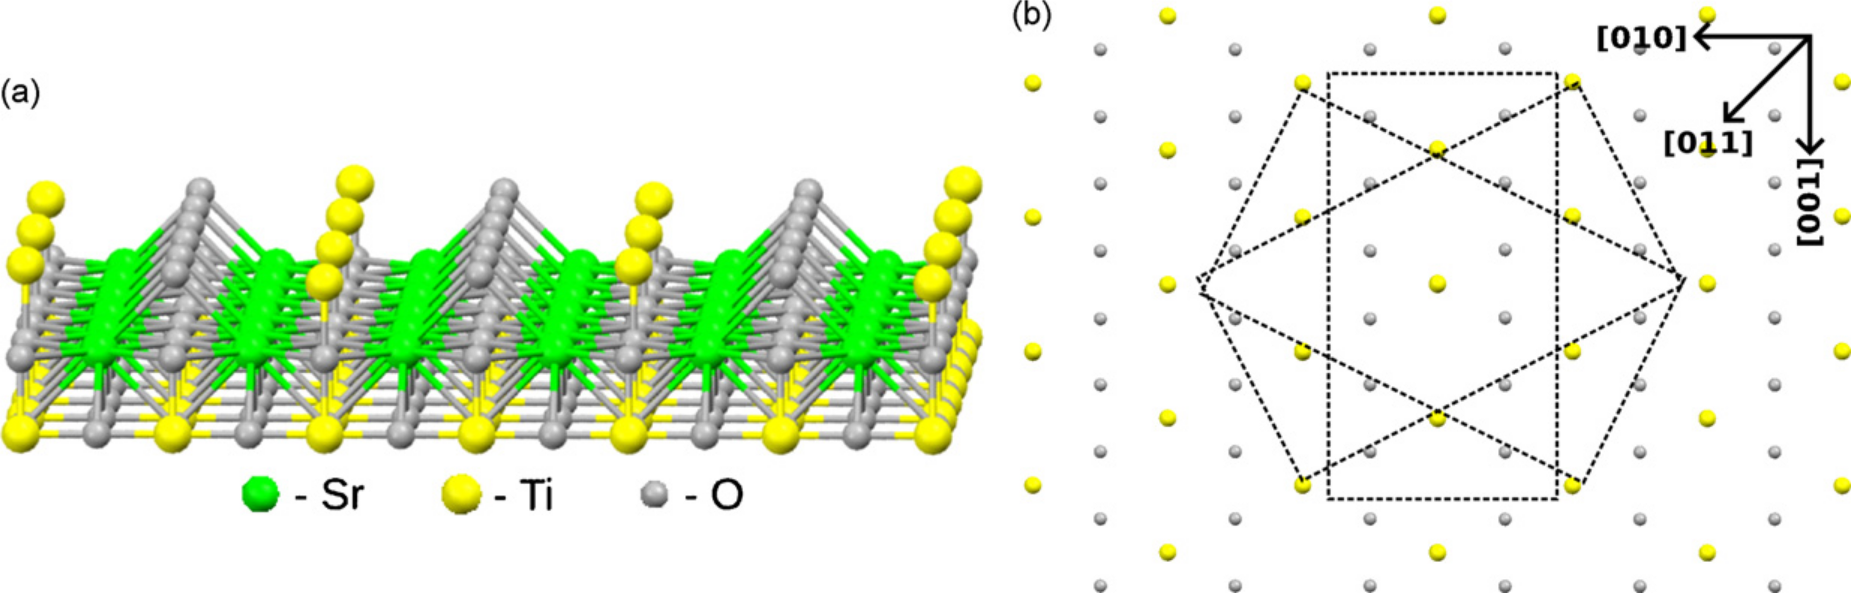
\includegraphics[width=\textwidth]{srtio3_c4x2}
    \caption[CdTe on c(4$\times$2) SrTiO\textsubscript{3} surface]{\label{fig:srtio3_c4x2}(a) Schematic showing the surface of the (100) SrTiO\textsubscript{3} with a c($4\times2$) surface reconstruction. (b) Schematic showing the uppermost layer of the reconstruction with the dashed lines being used to illustrate the closest geometrical fits of the (211) CdTe plane to this surface. The three orientations shown give rise to six grain orientations as a 180\degree~rotation of the (211) plane yields a different grain structure. This is a consequence of the fact that the single crystal (111) CdTe pole figure for a [211] film is one-fold symmetric (see \cref{fig:srtio3_sim_pole}b). Six other grain structures arise from a domain structure in the substrate surface reconstruction that would be schematically represented by a 90\degree{} rotation of \cref{fig:srtio3_c4x2}b. The Miller indices shown in the top right corner of the figure correspond to the crystallographic orientation of the underlying bulk (100) SrTiO\textsubscript{3} substrate.}
\end{figure}

Assuming that the orientation relationships between CdTe
and the surface reconstructions shown in \cref{fig:srtio3_c4x2,fig:srtio3_c6x2} are adhered
to then it becomes possible to experimentally predict the surface
reconstruction undergone by the substrates presented in this
work. It should be noted from \cref{fig:srtio3_c4x2}b that the c($4\times2$)
reconstruction is characterized by (211) CdTe grain alignment
along the substrate’s [010] and [001] directions. \Cref{fig:srtio3_pole}b
shows that this is not the case, ruling out this reconstruction for the
work presented here. It does not, however, rule out the possibility
of [211] CdTe grain growth if a film were deposited on such a
reconstruction. The c($6\times2$) reconstruction, on the other hand,
requires grain growth along the substrate’s [011] and [0$\overline{1}$1]
directions, consistent with the X-ray data. While we have no direct
evidence that the c($6\times2$) surface reconstruction formed, it is of
note that the anneal conditions used elsewhere\cite{Jiang1996} to obtain this
reconstruction are similar to those used here. While it should be
understood that predicting a film-substrate orientation relationship solely on the basis of a geometrical fit is somewhat na\"{\i}ve, it is well established that this scenario occurs more often than not.
\begin{figure}
    \centering
    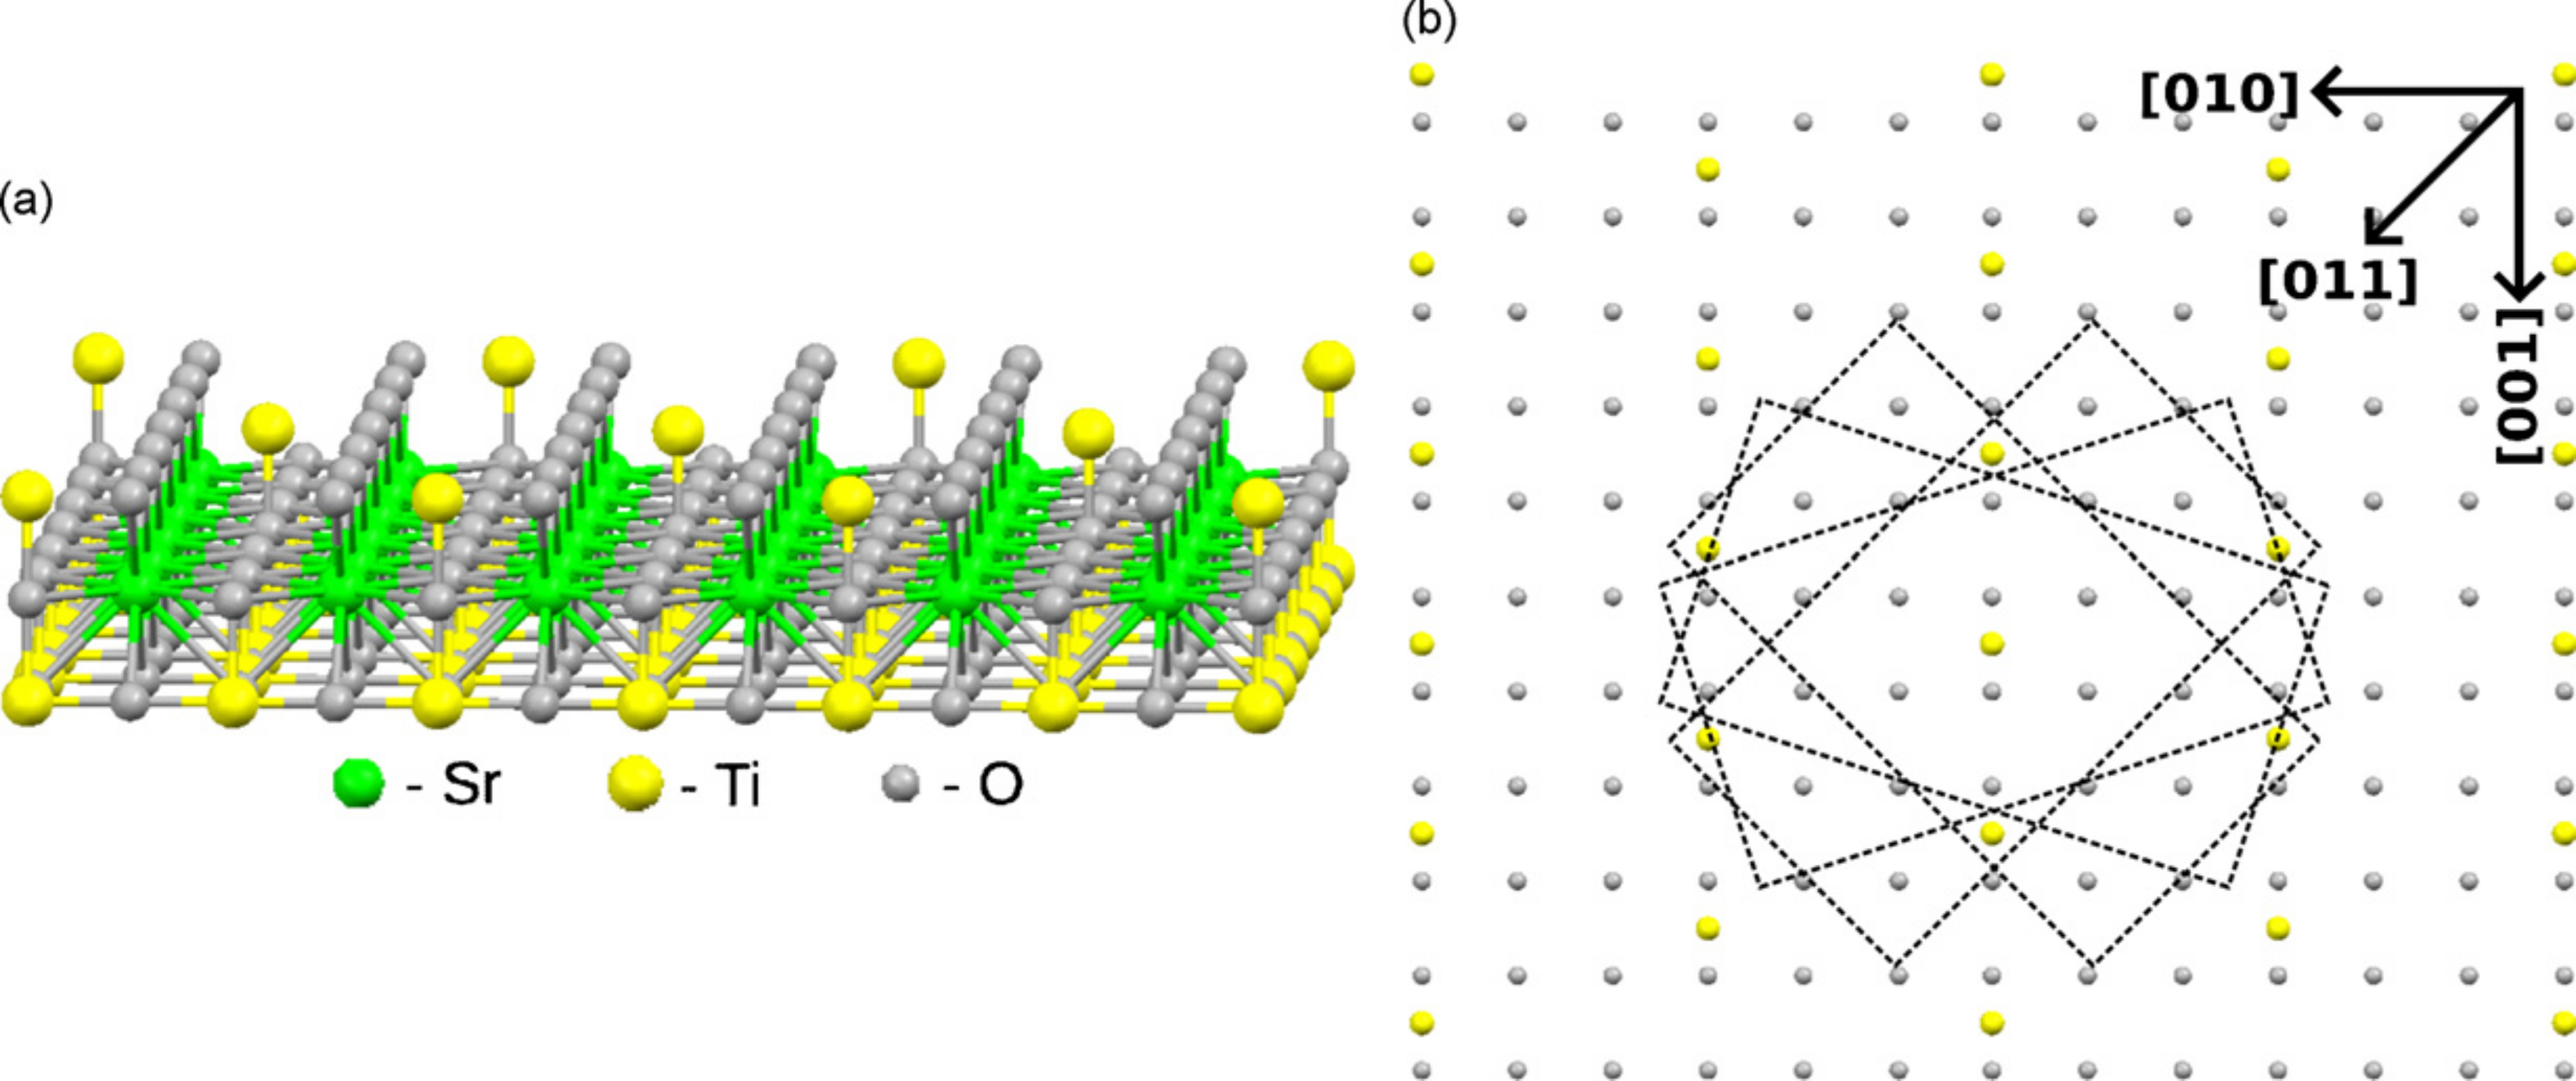
\includegraphics[width=\textwidth]{srtio3_c6x2}
    \caption[CdTe on c(6$\times$2) SrTiO\textsubscript{3} surface]{\label{fig:srtio3_c6x2}(a) Schematic showing the surface of the (100) SrTiO\textsubscript{3} with a c($6\times2$) surface reconstruction. (b) Schematic showing the uppermost layer of the reconstruction with the
        dashed lines being used to illustrate the closest geometrical fits of the (211) CdTe plane to this surface. The four orientations shown give rise to eight grain orientations as a
        180\degree{} rotation of the (211) plane yields a different grain structure. Eight other grain structures arise from a domain structure in the substrate surface reconstruction that
        would be schematically represented by a 90\degree~rotation of \cref{fig:srtio3_c4x2}b. Of these eight grains only four represent unique solutions as the grains forming along the [011] and [01$\overline{1}$]
        directions rotate into each other. The Miller indices shown in the top right corner of the figure correspond to the crystallographic orientation of the underlying bulk (100)
        SrTiO\textsubscript{3} substrate.}
\end{figure}

Even though both the [211] oriented films show pole figure
peaks in similar positions, the relative intensities of the peaks are
quite different. This is most easily seen by examining the
innermost ring of the pole figure where each of the twelve peaks
corresponds to a unique grain orientation. For both samples the
peaks on one side of the ring show greater intensities than on the
other. This effect, however, is much more pronounced for the pole
figure shown in \cref{fig:srtio3_pole}c. Here, the ratio of the integrated intensities
between the largest and smallest peak in the ring is 22 compared to
4 for the pole figure shown in \cref{fig:srtio3_pole}b. The fact that the terrace
width is approximately four times smaller for the film that shows
the most pole figure anisotropy suggests that the step edges
promote this preferential grain alignment. Consistent with this
explanation is the fact that the highest intensity peaks correspond
to the CdTe grain orientation having its [111] in-plane direction
normal to the step. The larger grain sizes exhibited by the surface
with smaller terraces are also expected within this scenario. This is
a simple consequence of the fact that, in the early stages of film
growth, there are more similarly oriented grains that are able to
merge into a single larger grain as is expected for an island growth
mechanism. With a sizeable effect being observed between the two
reconstructed surfaces having a miscut difference of only 0.358, the
potential exists to amplify this effect using a substrate with a
significantly larger miscut.

The results presented here demonstrate that the reconstructed
surface of (100) SrTiO\textsubscript{3} profoundly alters the grain structure of
CdTe films. While it is not unusual for the grain structure to be
transformed by the presence of a step-terrace morphology, it is
unprecedented for SrTiO\textsubscript{3}’s atomic-scale reconstructions to pro-
mote a film with an alternative heteroepitaxial relationship. For
the case of (100) SrTiO\textsubscript{3}, there seems to be a disconnect between
the research advocating a step-flow growth mode and the wide
array of atomic-scale surface reconstructions allowed, with the
latter not considered as a determining factor in the film quality
achieved. This may be due to the relatively high growth
temperatures used in the fabrication of oxide thin films. In this
case, the thermal energy available likely facilitates a local
rearrangement of surface atoms in response to the addition of
adatoms. This is certainly the case for the homoepitaxial growth of
silicon where the surface reconstruction gives way to bulk
crystalline ordering for temperatures in excess of 300\celsius{}\cite{Gossmann1985}.
For the low growth temperatures used in the fabrication of these
CdTe films the surface reconstruction is likely locked in place,
forcing CdTe to accommodate itself on the reconstructed surface.
The sparsely populated nature of such a surface should make it
prone to alternative epitaxial relationships as the interface would
not consist of an abrupt boundary, but instead, of an amalgamation
of two interpenetrating layers. Consistent with this explanation is
the fact that different (100) SrTiO\textsubscript{3} surface reconstructions give
rise to palladium nanodots having variable orientations and
faceting\cite{Silly2005b}.
\section{Implications for Symmetry and Energy at Epitaxial Surfaces}
While the results presented here don't explicitly improve the growth of the CdTe thin films, they do add to the understanding of the role of the interface in epitaxy. In all the cases presented here, the substrate used for epitaxial growth has a nominal orientation of (100), with very small miscut of less than 1\degree. Despite a fixed orientation for the substrate, the thin surface net presented to the epitaxial thin film dominates the nucleation and growth orientation. These results show that it is possible to leverage high temperature surface reconstructions in order to completely transform a given substrate. If a reconstruction can be created at high temperature and then locked-in at the growth temperature substrates that don't immediately appear to be an epitaxial match can end up presenting an ideal template for growth. The additional symmetry breaking that is available for offcut substrates can widen the range of acceptable substrates, by triggering a step-flow growth mode suppressing unwanted orientations.

For this type of surface net epitaxy to yield the most benefit, surface science research must investigate the zoo of surface reconstructions possible on the commercially available complex oxides. Many of the higher element complex oxides (YAG, YSZ, GGG etc.) have little to no literature examining their surface reconstructions or their behaviour when miscut. Phase diagrams of such surfaces would be highly beneficial in predicting good matches for epitaxy.
\chapter{CdTe Nanowire Growth on Sapphire}
\section{Introduction} \label{sec:cdtenanowires}
A topic of substantial interest in semiconductor physics in recent years has been the potential of confined dimensional materials such as nanowires, particularly through the vapour-liquid-solid (VLS) growth process.
As the research group had been successful at producing thin films of CdTe, experiments were attempted in the production of CdTe nanowires using a number of metal catalysts.

CdTe VLS nanowires were successfully grown using the PLD process and several insights were gained into the role of energetics at the epitaxial growth surface, and how they can affect nanowires during growth.
This work was published as:\\
\fullcite{Neretina2008b} \cite{Neretina2008b}.\\
This work was done in close collaboration with Dr. Robert Hughes and Dr. Svetlana Neretina. Dr. Hughes grew the samples of interest, Dr. Neretina performed the SEM imaging and 2DXRD measurements and I performed the statistical analysis of the nanowire SEM images and numerically modelled the growth process.
\section{Experimental}
The experimental results and procedures presented here will focus on those nanowires derived from Bi\textsubscript{2}Te\textsubscript{3} catalytic seeds deposited on pristine (0001) sapphire substrates.
The results obtained will then be compared to the CdTe nanowires, described elsewhere\cite{Neretina2007b}, obtained using bismuth catalytic seeds deposited on polyvinyl alcohol or terpineol treated (0001) sapphire substrates.

The Bi\textsubscript{2}Te\textsubscript{3} seeds were prepared using the PLD process (GSI Lumonics IPEX-848 excimer laser at 248~nm, laser energy density 2 J~cm\textsuperscript{-2}, laser spot size  1.2\(\times\)1.2 mm\textsuperscript{2}).
The target used was prepared in-house from commercially available Bi\textsubscript{2}Te\textsubscript{3} pieces (99.999\% purity).
These pieces were
melted in a cylindrical graphite mould that was machined to sizes able to yield a 1 inch target weighing approximately 10 g.
This procedure was carried out in an argon background gas.
Before the deposition, the sapphire substrate was heated to 400\celsius{} and held there for 10~min in an oxygen background pressure of 300~mTorr.The substrate was then cooled to room temperature where a 20~\AA{} thick film of Bi\textsubscript{2}Te\textsubscript{3} was deposited.
This deposition lasted 35 s at a laser repetition rate of 3~Hz.
Once deposited, the film was then heated to 370\celsius{} where, over the course of 10 min, it would dewet forming Bi\textsubscript{2}Te\textsubscript{3} seeds.
At this point, a 30~sccm helium flow was introduced into the chamber such that the pressure was maintained at 400~mTorr.
Material from a rotating CdTe target, grown using the Bridgman method, was then deposited onto the substrate for time intervals typically in the range of 30--45~min at a laser repetition rate of 8~Hz.
The nanowires were then allowed to cool to room temperature in the helium ambient.

\section{Results and Discussion}
\Cref{fig:nanocdte_bite} shows an SEM image, of the Bi\textsubscript{2}Te\textsubscript{3} catalytic seeds formed on the (0001) sapphire substrate.
The seeds show a substantial size distribution with diameters as large as 150~nm.
While these seeds show enhanced stability, they are still prone to evaporation and will disappear completely if the CdTe deposition is delayed by approximately 10~min.
As was the case for the bismuth catalysts, the Bi\textsubscript{2}Te\textsubscript{3} seeds gain stability from exposure to the cadmium/tellurium flux.
It is also likely that the seeds shown in the image are somewhat different from those available when nanowire growth commences as the time required to cool these seeds to room temperature provided ample opportunity for further evaporation and Ostwald ripening.
\begin{figure}
 \centering
 \begin{subfigure}[t]{0.47\textwidth}
  \centering 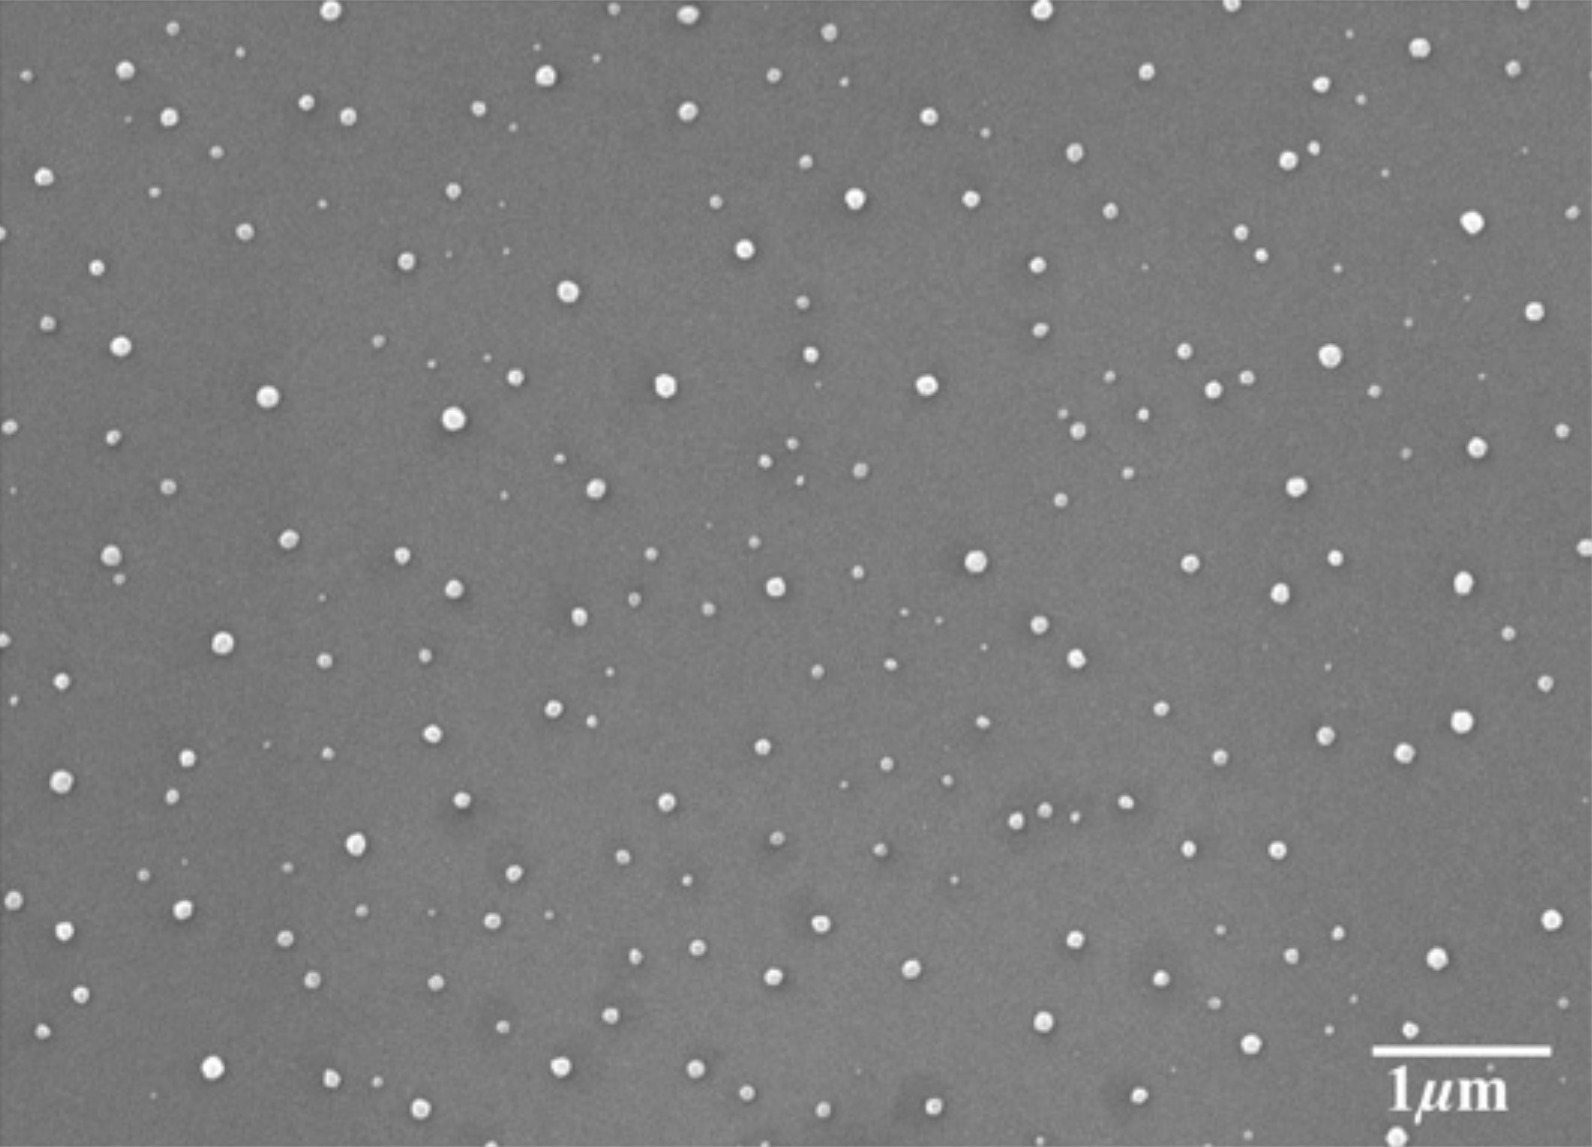
\includegraphics[width=\textwidth]{nanocdte_bite}
  \caption{\label{fig:nanocdte_bite}SEM image of the Bi\textsubscript{2}Te\textsubscript{3} seeds that were used as catalysts for CdTe nanowires.}
 \end{subfigure}\quad%
 \begin{subfigure}[t]{0.47\textwidth}
  \centering 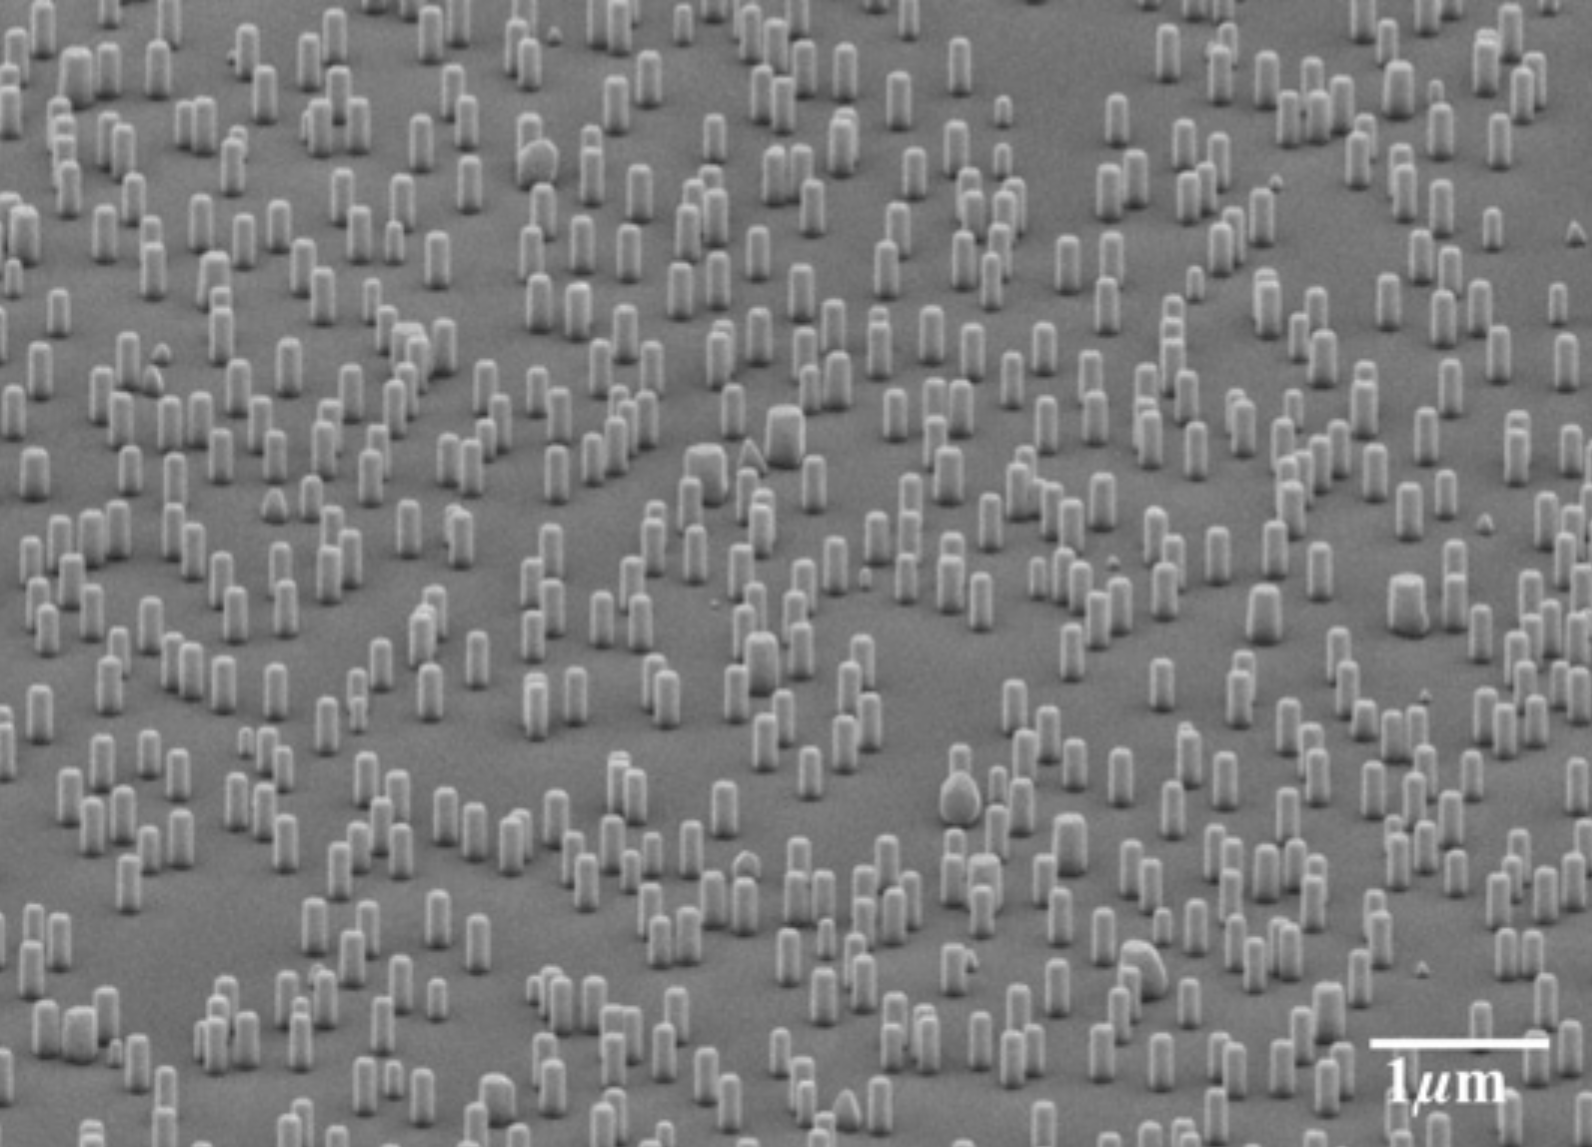
\includegraphics[width=\textwidth]{nanocdte_nanowires}
  \caption{\label{fig:nanocdte_nanowires} SEM image of CdTe nanowires derived from Bi\textsubscript{2}Te\textsubscript{3} catalytic seeds presented from a 70\degree{} tilt side view.}
 \end{subfigure}
 \caption{\label{fig:nanocdte_sem}SEMs of seeds and resulting wires.}
\end{figure}

\Cref{fig:nanocdte_nanowires} shows an SEM image of the CdTe nanowires derived from Bi\textsubscript{2}Te\textsubscript{3} seeds.
In many respects, these nanowires are indistinguishable from those grown using bismuth seeds in conjunction with an alcohol-altered surface\cite{Neretina2007b}.
The two methods both yield vertically aligned nanowires that are highly faceted, share an epitaxial relationship with the substrate and grow without a two-dimensional planar layer.
The nanowires are identical from a structural standpoint as well, exhibiting the wurtzite crystal structure instead of the bulk zincblende phase.
\Cref{fig:nanocdte_polefigure} shows a pole figure that includes contributions from both the (111) zincblende and (0002) wurtzite planes.
Both phases give rise to a peak in the centre of the pole, but a zincblende phase must also give rise to a ring of three peaks at the outer extent of the pole.
For the pole figure shown no such peaks are observed, but in general a small zincblende signature was visible.
The three small peaks that do appear in the pole figure are associated with the sapphire substrate.
\begin{figure}
 \centering 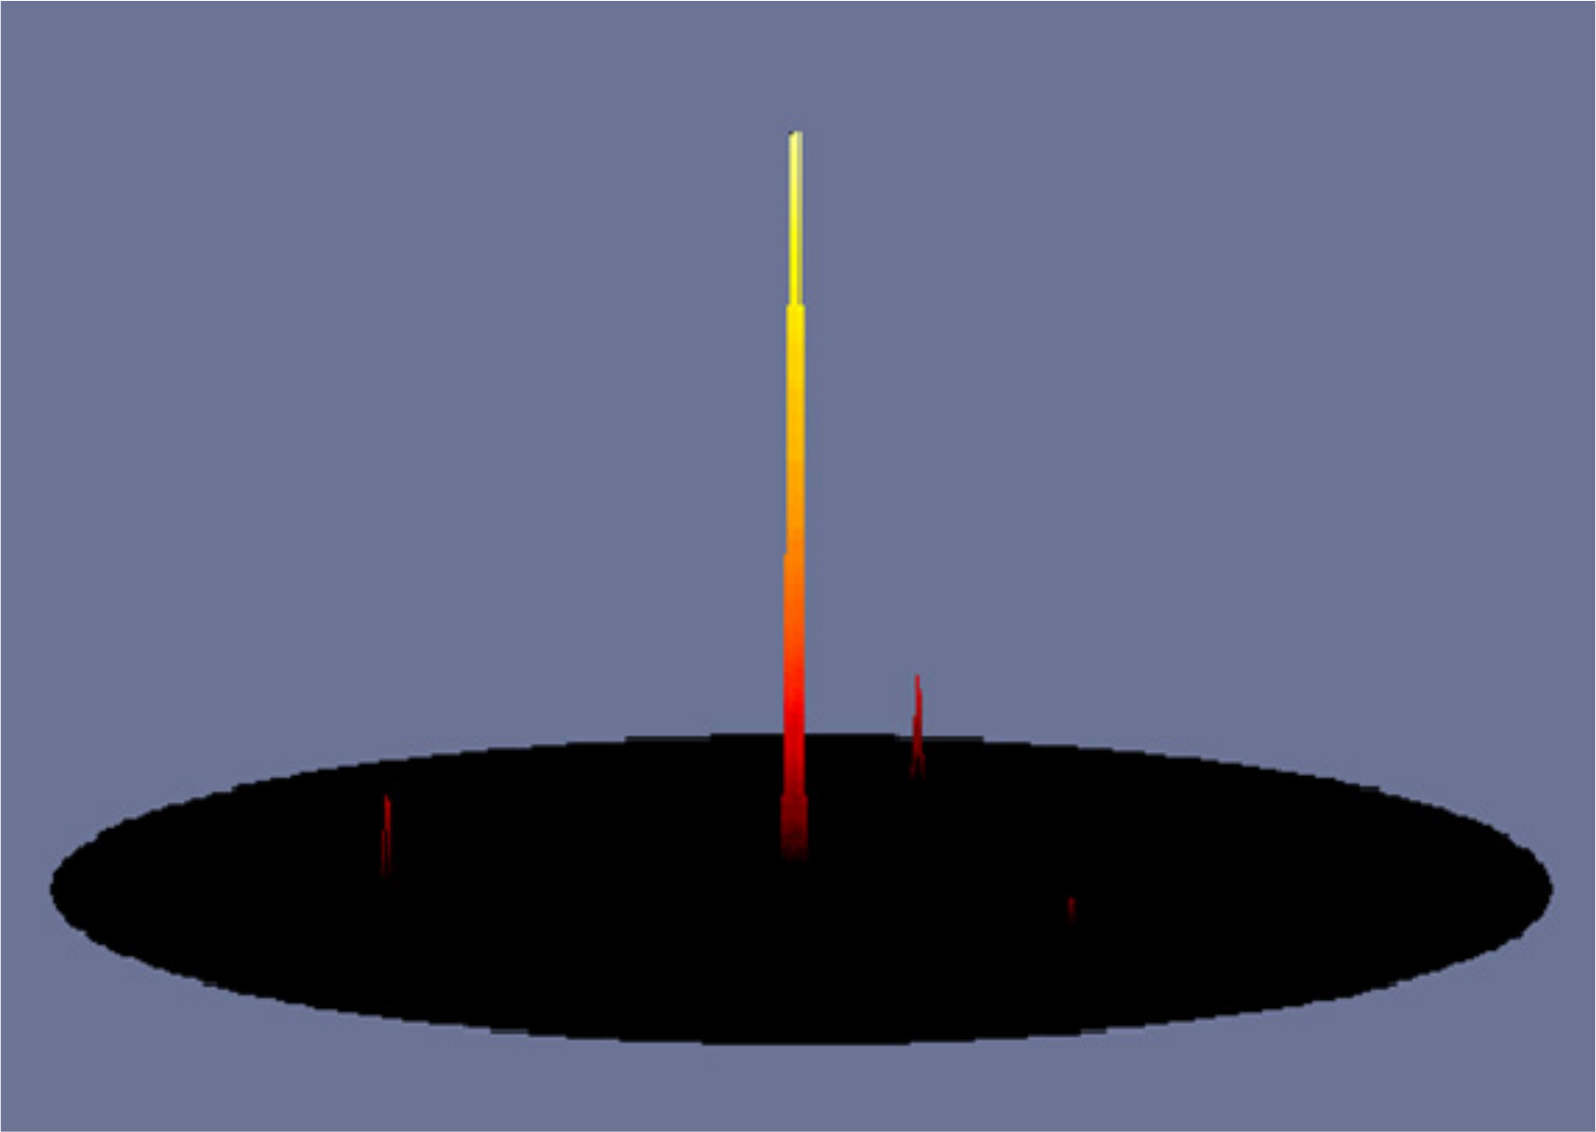
\includegraphics[width=0.6\textwidth]{nanocdte_polefigure}
 \caption[Pole figure of CdTe nanowires]{\label{fig:nanocdte_polefigure}CdTe pole figure results for 2\straighttheta{}values that include contributions from both the (111) zincblende and (0002) wurtzite phases.
  The pole figure shows no evidence of a zincblende phase.
  The three small peaks originate from the (0001) sapphire substrate.}
\end{figure}

Even though these Bi\textsubscript{2}Te\textsubscript{3} catalysed nanowires share many similarities with those derived from the bismuth seeds deposited on an alcohol-altered surface, there do exist substantial differences.
One of the most striking differences is the nanowire size distribution observed in the SEM images of \cref{fig:nanocdte_SEM2}.
This size distribution is quantified by the colour map presented in \cref{fig:nanocdte_stats}a.
It shows a nanowire height versus diameter distribution for the Bi\textsubscript{2}Te\textsubscript{3} seeded nanowires.
It is quite clear from the map that larger diameter nanowires exhibit higher axial growth rates than those with smaller diameters.
\Cref{fig:nanocdte_stats}b shows the same distribution for nanowires derived from bismuth seeds deposited on an alcohol-altered surface.
A comparison of the two colour maps shows that the alcohol-altered surface gives rise to a narrower size distribution.
It is also apparent from the distributions that the Bi\textsubscript{2}Te\textsubscript{3} seeded nanowires are of larger diameter with values typically in the range of 80--200~nm.
Also different is the fact that the Bi\textsubscript{2}Te\textsubscript{3} nanowire height is not limited to 300~nm.
Instead the nanowires grow longer while exhibiting substantial growth in the lateral direction (\cref{fig:nanocdte_lateral}).
Moving away from the optimum growth conditions gives rise to other differences between the two nanowire growth procedures.
First, nanowires formed at the substrate's edge have slanted tops where the direction of the slant at the left and right edges of the substrate point in opposite directions (\cref{fig:nanocdte_slanted}).
Also of note is the fact that the nanowire's cross-section is no longer hexagonal, but instead elongates along the direction of the slant.
Second, at high growth rates Bi\textsubscript{2}Te\textsubscript{3} seeded nanowires show distinct tapering (\cref{fig:nanocdte_tapered}).
\begin{figure}
 \centering 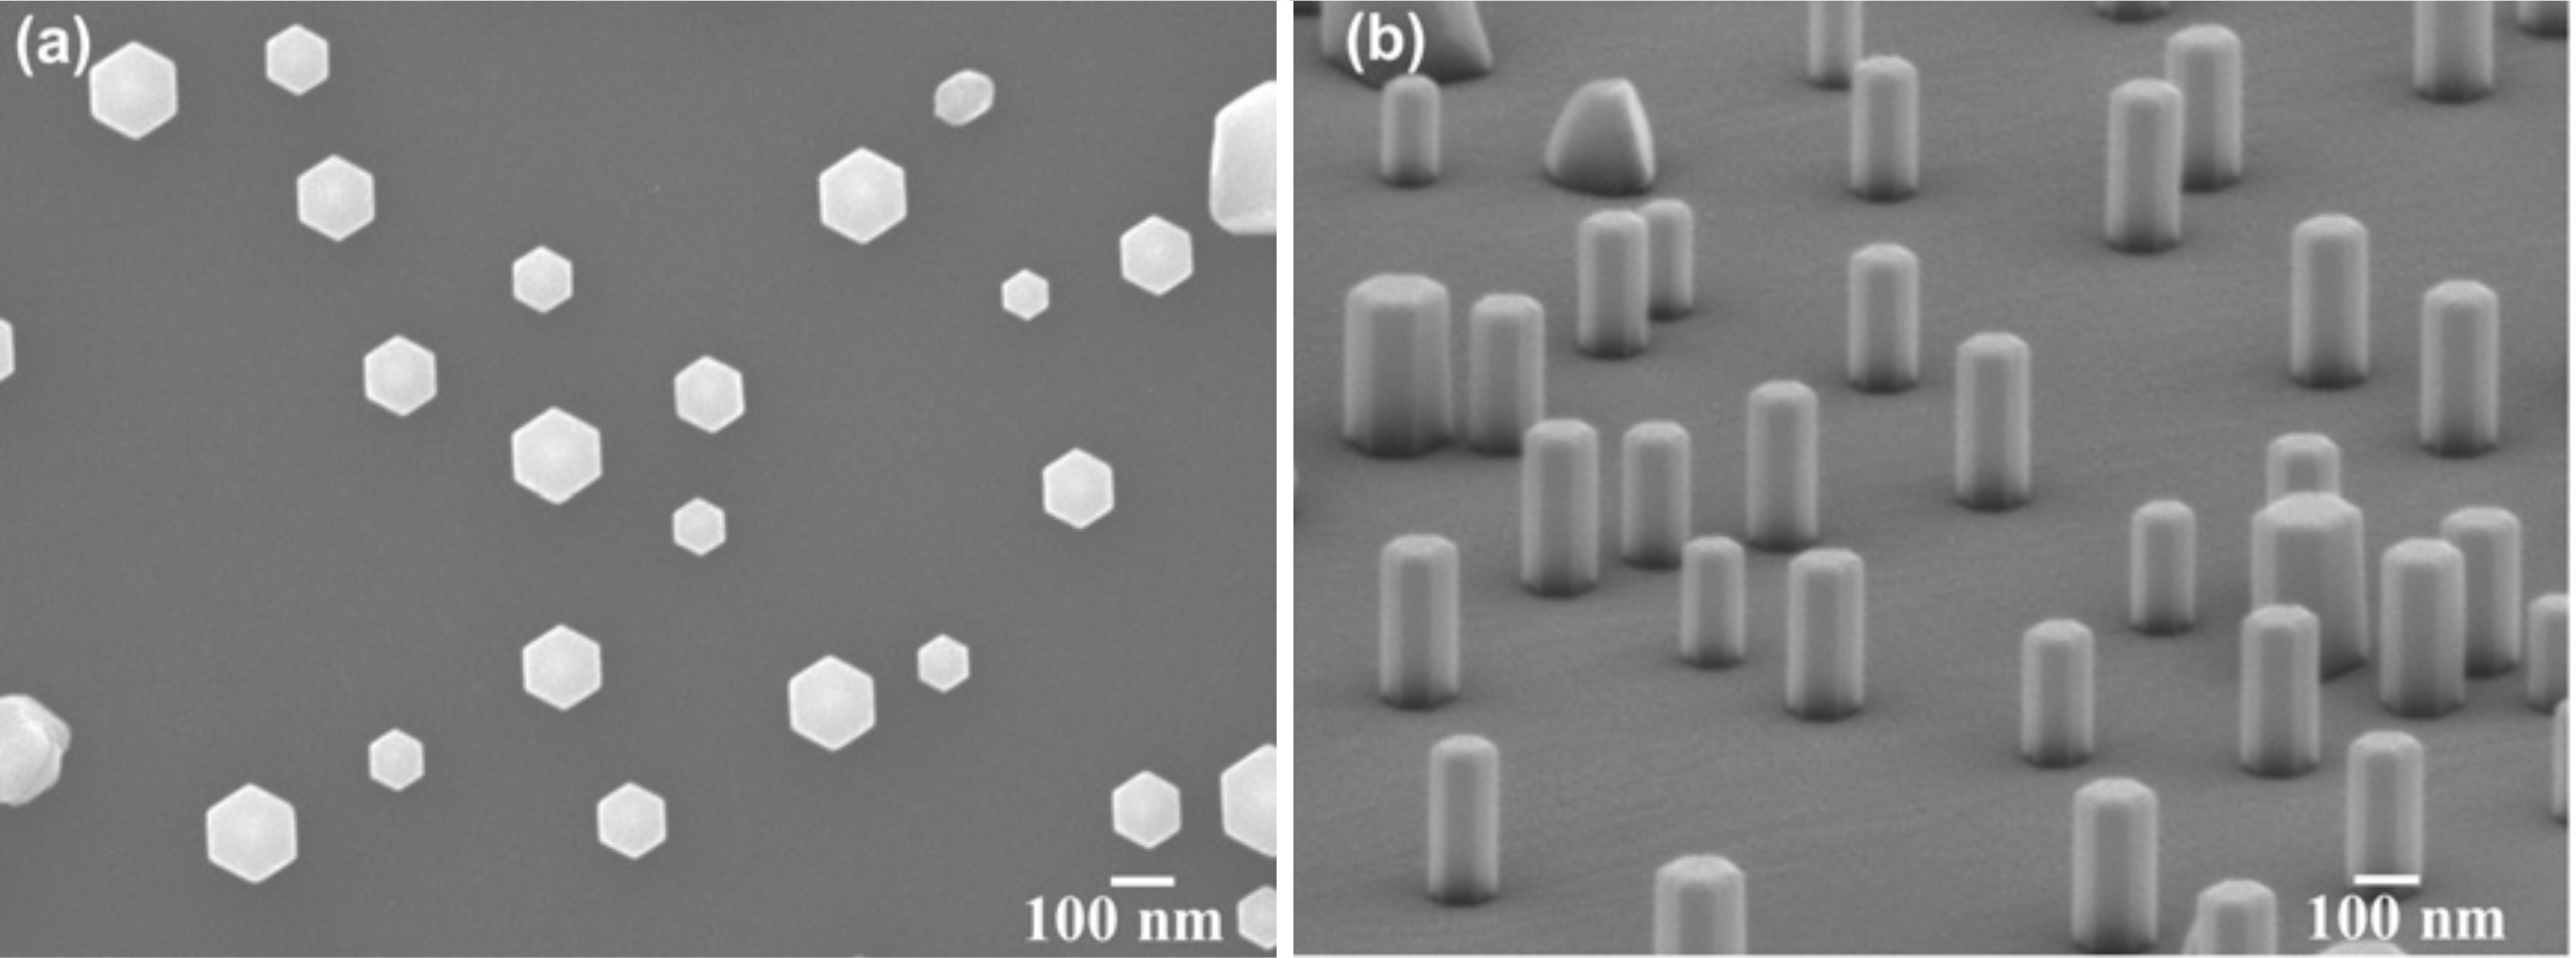
\includegraphics[width=\textwidth]{nanocdte_SEM2}
 \caption[SEM image of CdTe nanowires]{\label{fig:nanocdte_SEM2}SEM images of CdTe nanowires from a (a) top and (b) side view (70\degree{} tilt).
  Highly faceted wires exhibit a substantial variation in both heights and diameters.}
\end{figure}
\begin{figure}
 \centering 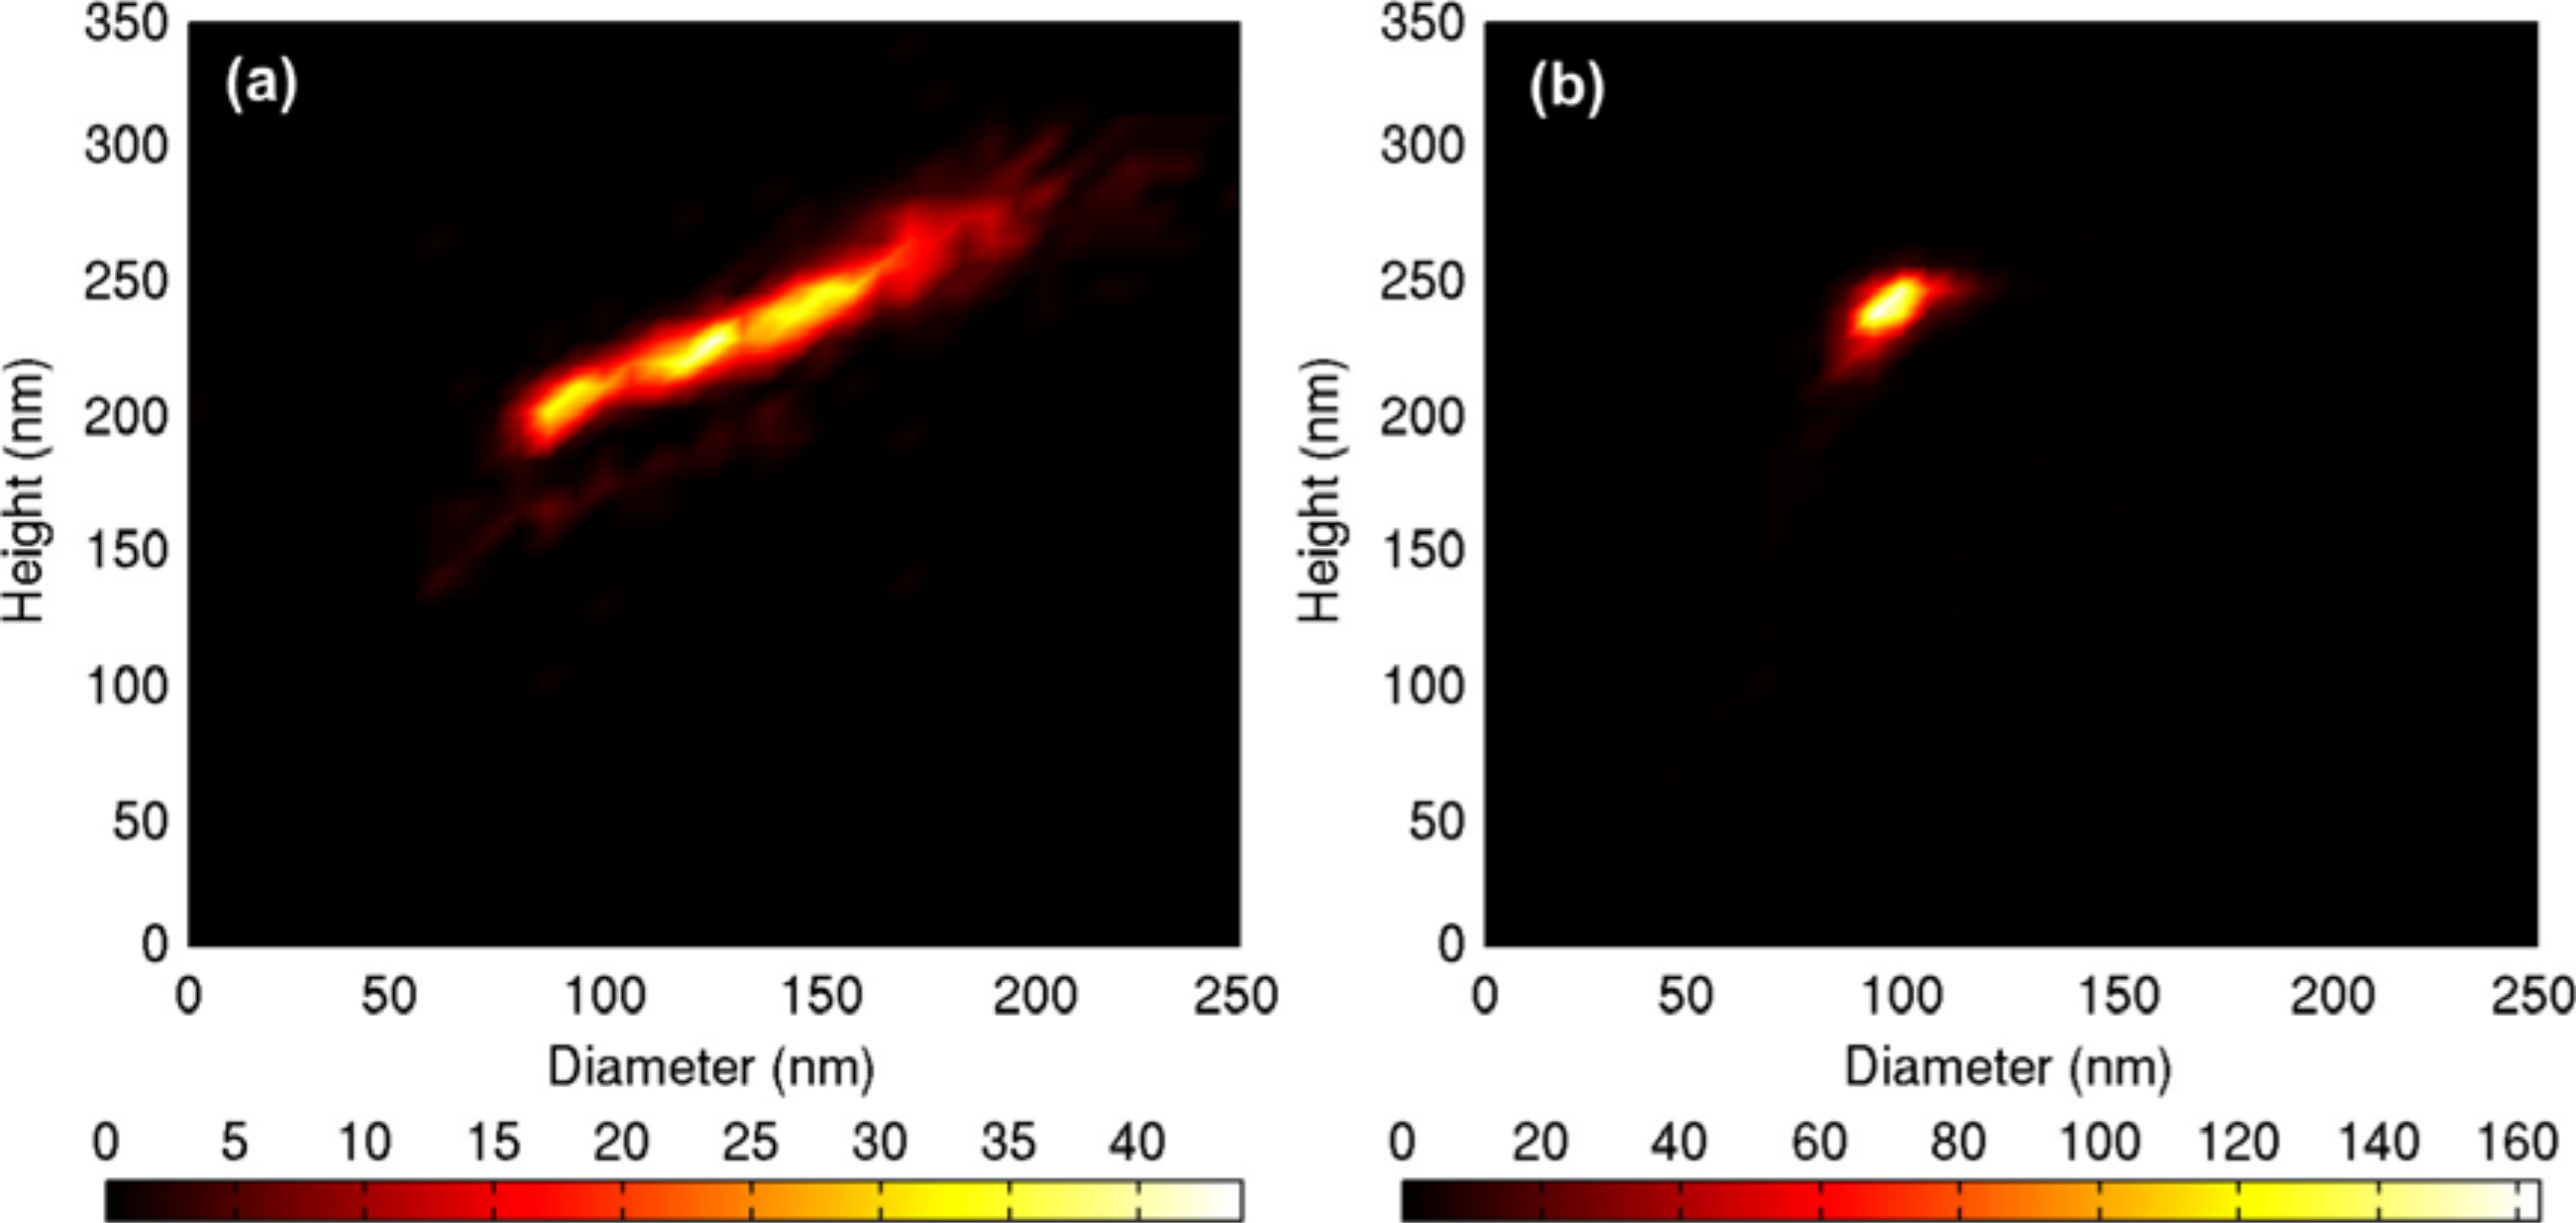
\includegraphics[width=\textwidth]{nanocdte_stats}
 \caption[CdTe nanowire dimension colourmap]{\label{fig:nanocdte_stats}Colour map showing the nanowire height versus diameter size distribution for nanowires derived from (a) Bi\textsubscript{2}Te\textsubscript{3} catalytic seeds and (b) bismuth seeds deposited on an alcohol-altered surface.
  The maps were generated from the measured dimensions of (a) 1344 and (b) 966 nanowires.
  The colour bar below each figure denotes the number of times a nanowire of a given dimension is observed.
  The Bi\textsubscript{2}Te\textsubscript{3} seeded nanowires exhibit a broader size distribution and sizes that are, in general, larger than the bismuth seeded wires.}
\end{figure}
\begin{figure}
 \centering 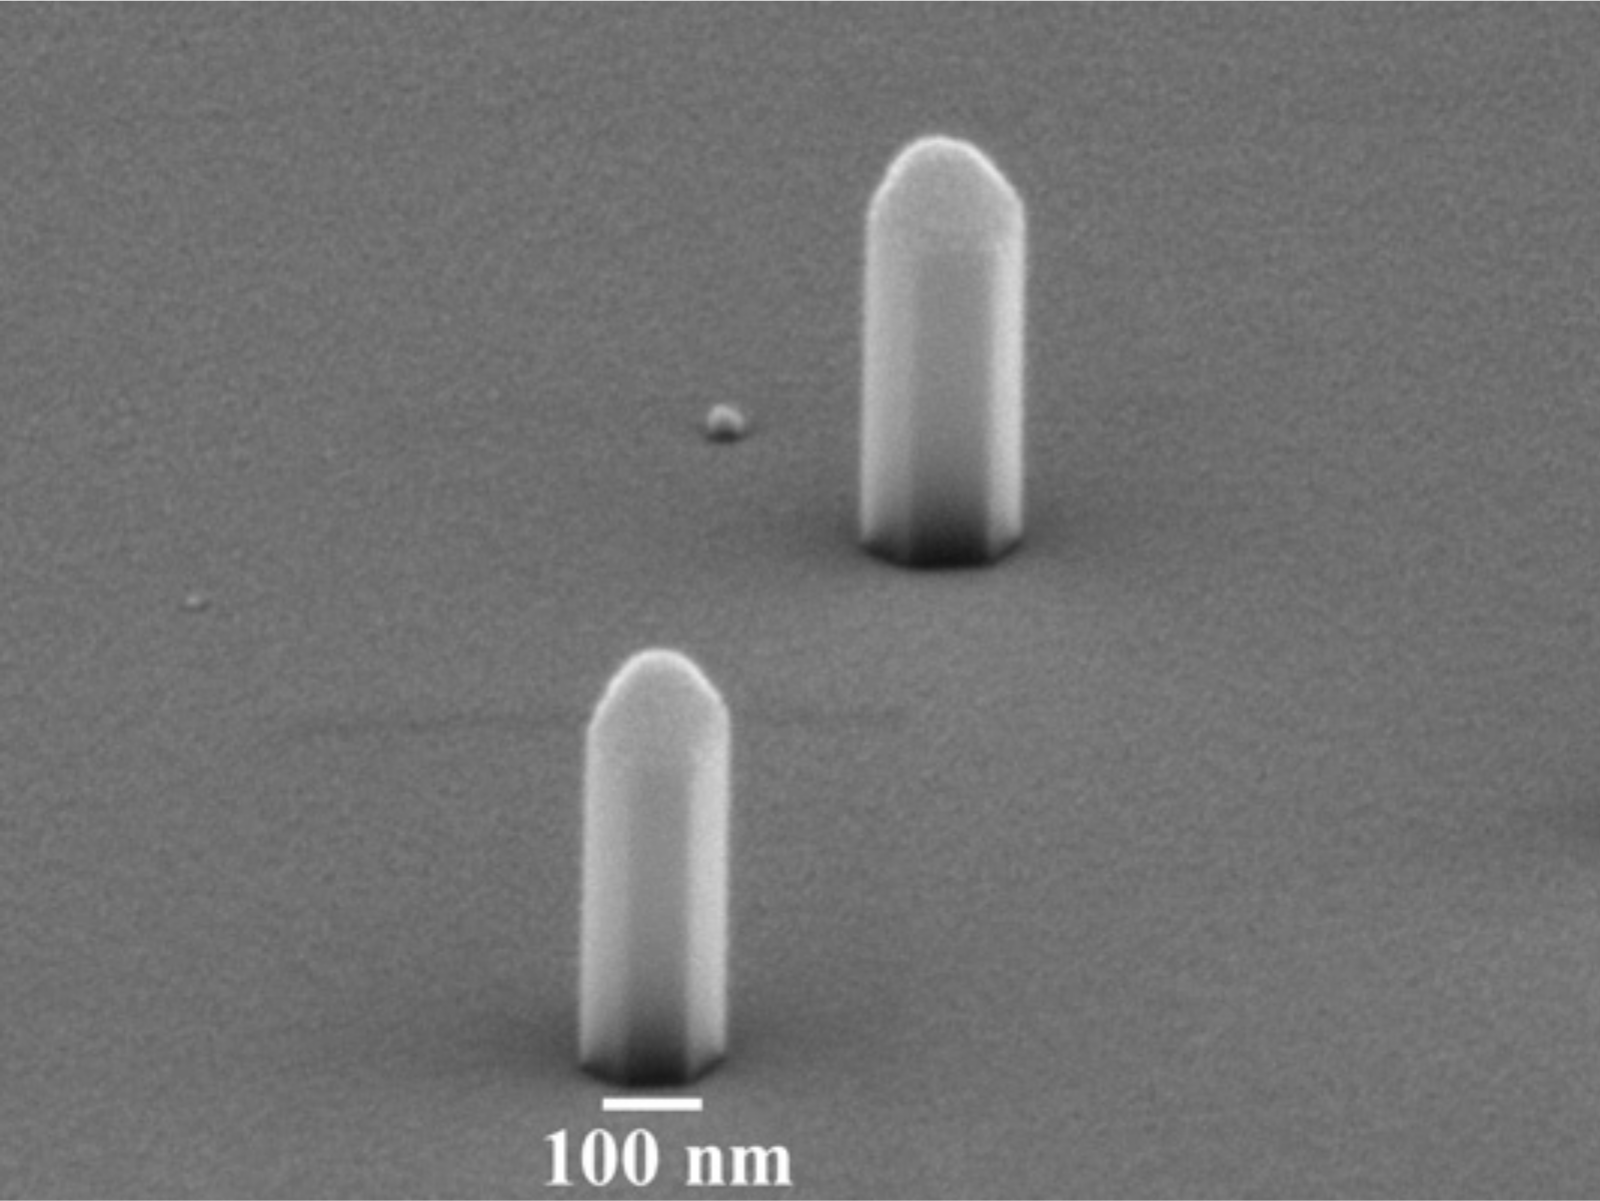
\includegraphics[width=0.6\textwidth]{nanocdte_lateral}
 \caption[CdTe nanowire lateral growth]{\label{fig:nanocdte_lateral}SEM images of CdTe nanowires deposited using extended growth times where increases to the height are met with substantial lateral growth.}
\end{figure}
\begin{figure}
 \centering 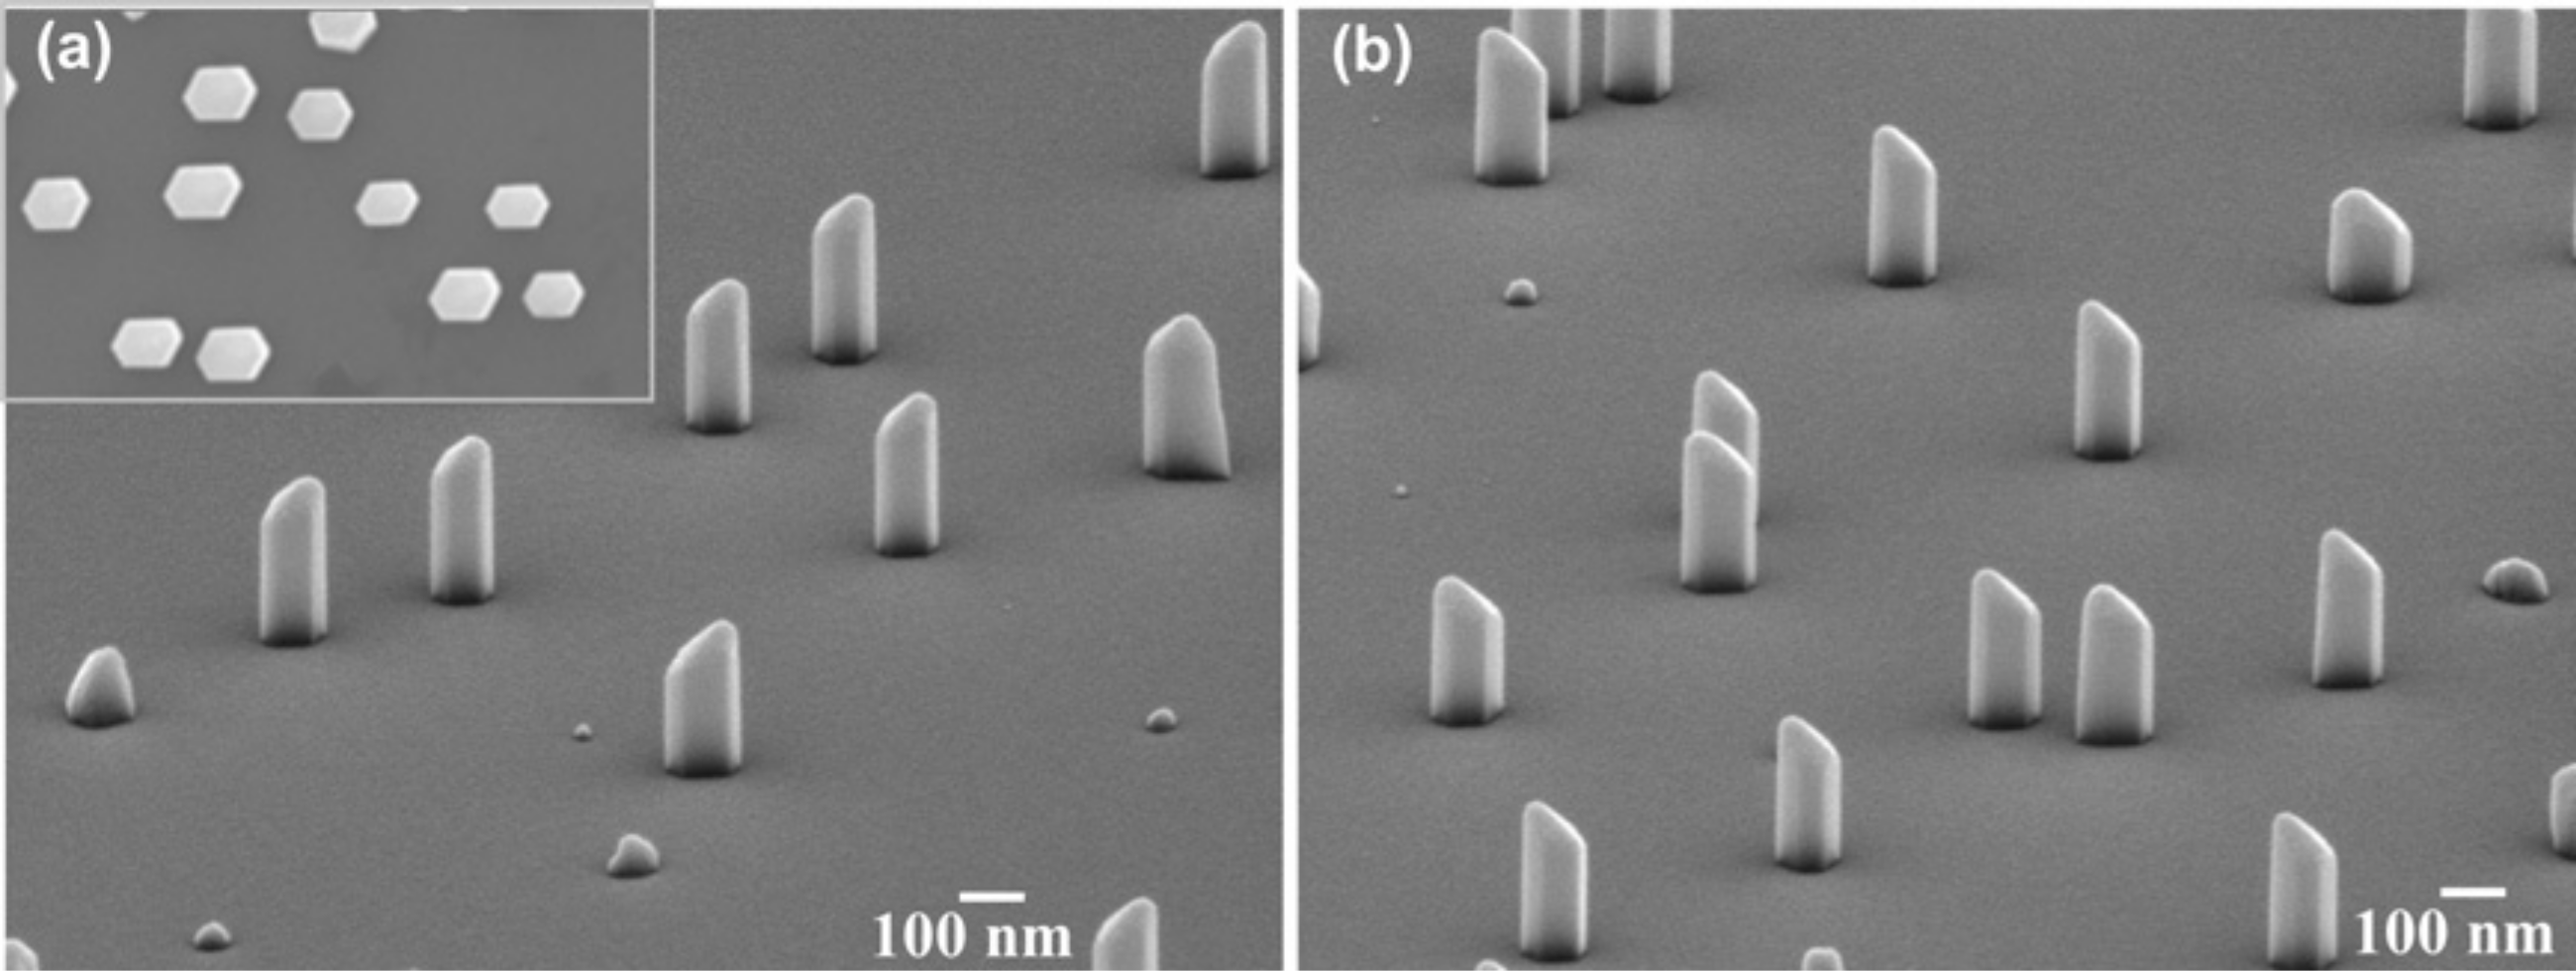
\includegraphics[width=\textwidth]{nanocdte_slanted}
 \caption[CdTe nanowires with slanted tops]{\label{fig:nanocdte_slanted}SEM images of CdTe nanowires with slanted tops that have formed at the (a) left and (b) right edge of the substrate.
  The tilt is in opposite directions.
  The top views of these nanostructures, shown in the inset to (a), indicate that the hexagonal cross-sections are elongated in the horizontal direction.}
\end{figure}
\begin{figure}
 \centering 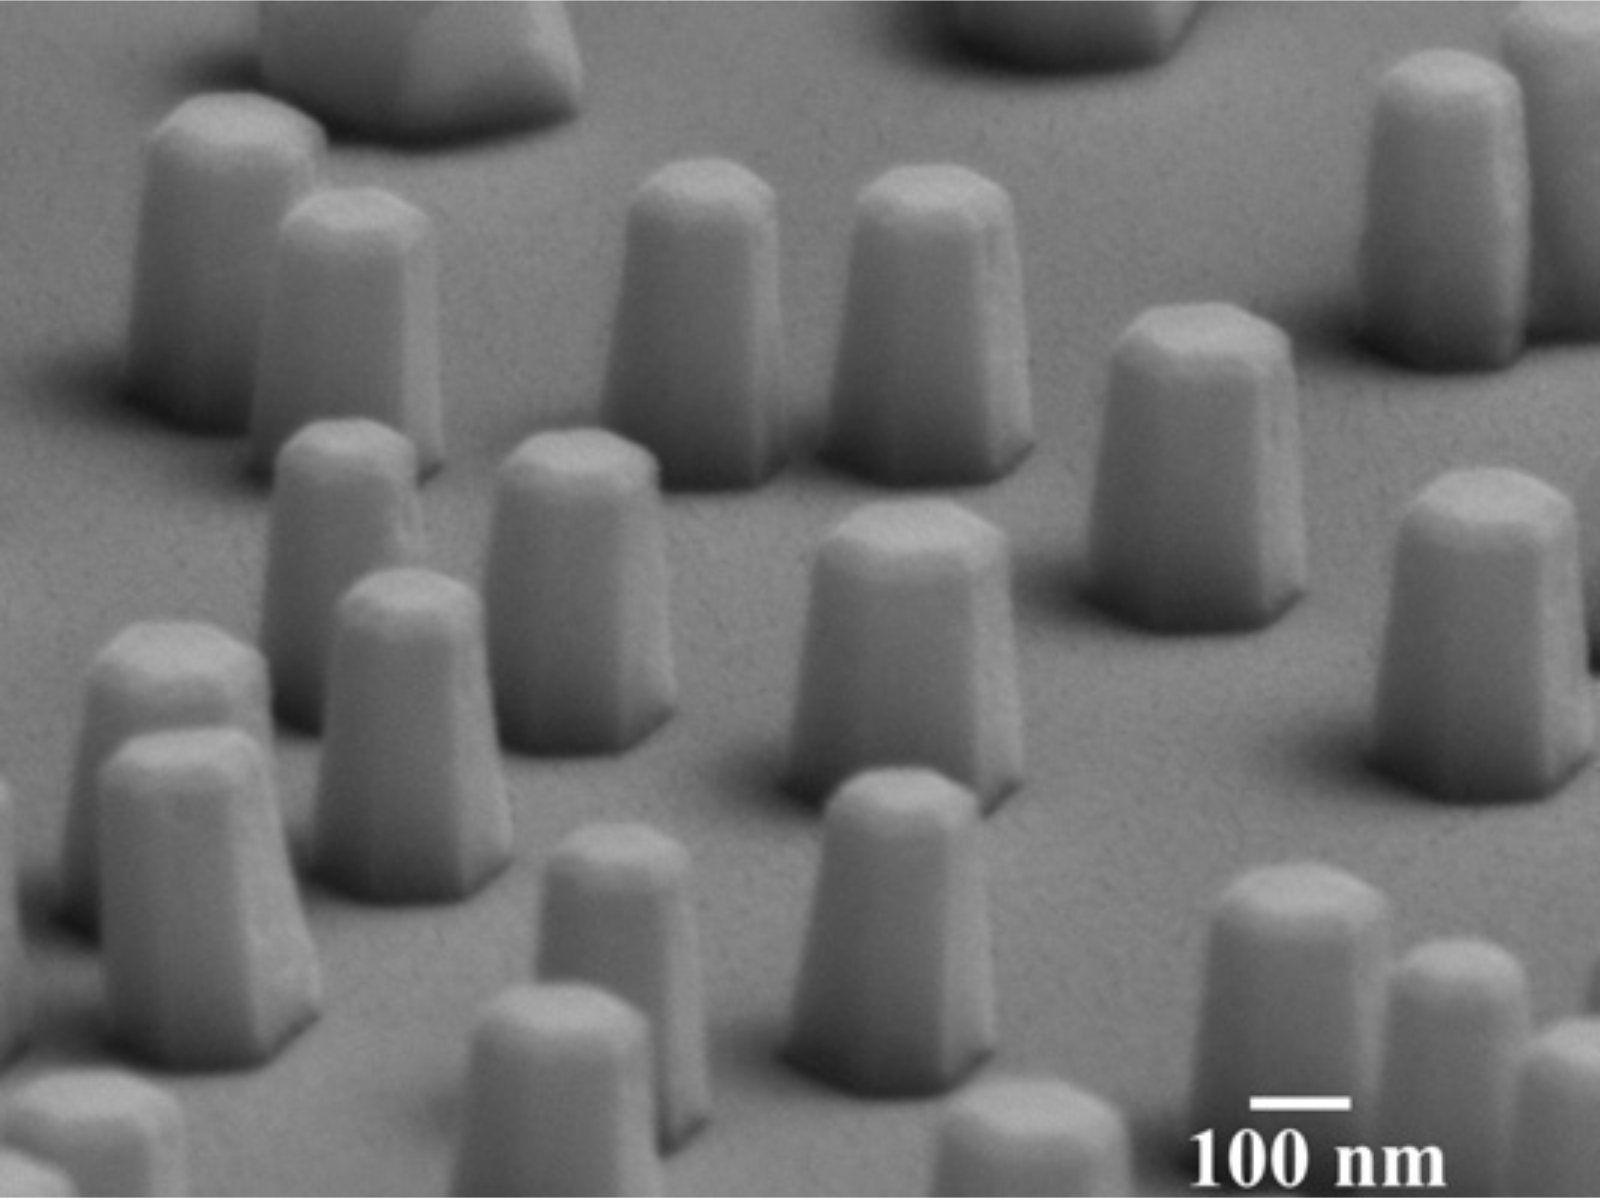
\includegraphics[width=0.6\textwidth]{nanocdte_tapered}
 \caption{\label{fig:nanocdte_tapered}SEM image showing tapered CdTe nanowires.}
\end{figure}
This work combined with our previous results has demonstrated that CdTe nanowire structures can originate from catalytic seeds derived from two separate processes, with each of these processes having advantages and disadvantages.
Bismuth seeds, in combination with an alcohol-altered surface, give rise to superior nanowire uniformity, but there exist nanowire height limitations and fabrication can only proceed using volatile catalytic seeds maintained in a narrow window of processing parameters.
The Bi\textsubscript{2}Te\textsubscript{3} seeds are much more stable at the temperatures needed to initiate CdTe nanowire growth.
This makes nanowire production possible without the cumbersome alcohol pre-treatment of the substrate's surface.
The main disadvantage is that the nanowire size and shape distributions are severely compromised.

Over one hundred samples have been characterized for each of the two nanowire deposition methods.
As a result, nanowire fabrication has been attempted over a broad range of growth conditions.
Thus, the features presented here as unique to the Bi\textsubscript{2}Te\textsubscript{3} initiated nanowires have been shown to decisively differentiate themselves from those observed using bismuth seeds deposited on an alcohol-altered surface.
If, as expected, both the bismuth and Bi\textsubscript{2}Te\textsubscript{3} catalytic seeds assume the same composition once exposed to a flux of cadmium and tellurium then the differences observed between the two methods must be attributed to the presence or absence of an alcohol-altered substrate surface.
It is our conjecture that this can be done within the confines of the existing nanowire growth modes.

For both nanowire deposition methods the catalytic seeds are derived from a thin film that dewets at elevated temperatures.
Once formed, these seeds are subject to Ostwald ripening, where there is an exchange of atoms along the substrate's surface with larger seeds growing at the expense of smaller ones\cite{Raab2000a,Li2003b}.
The effectiveness of this process is governed by the adatom's surface diffusion length given by the square root of the product of its diffusion coefficient and lifetime.
If this length is larger than the separation between seeds then Ostwald ripening proceeds in the usual manner where, as time progresses, there is an increasing variation in seed size.
On the other hand, if this length is reduced to where atoms liberated from one seed evaporate before encountering a second one, then a narrow size distribution will be maintained, but accompanied by a continuous reduction in the seed's diameter.

It is clear from our results that the pristine substrate used for the Bi\textsubscript{2}Te\textsubscript{3} seeds leads to sufficient surface mobility for Ostwald ripening to broaden the distribution of seed diameters.
Due to the higher volatility of tellurium we expect that this ripening process will result in bismuth-rich seeds.
Indeed, the binary phase diagram indicates that the growth temperature is too low for the seeds to melt unless there is first a substantial loss of tellurium\cite{MassalskiTBMurrayJL1986}.
The combination of Ostwald ripening in conjunction with evaporation leads to bismuth-rich catalytic seeds of different sizes which in turn cause nanowires of varying diameters.
Corrupting the surface with alcohol alters this process by dramatically reducing the surface mobility; this increases the lifetime of the seed on the surface and frustrates the Ostwald ripening process, i.e., any bismuth atoms liberated from an individual seed are backscattered to the original seed or evaporate from the surface before reaching a second seed.
With the ripening process halted, the distribution of seed diameters remains narrow, ultimately giving rise to a narrow distribution of nanowires.

With the catalytic seeds in place and exposed to a flux of cadmium and tellurium atoms it is expected that both the bismuth and Bi\textsubscript{2}Te\textsubscript{3} seeds will evolve to the same ternary composition.
While the ternary phase diagram for the cadmium/tellurium/bismuth system is unknown, it is well established that individually both tellurium and cadmium are soluble in bismuth\cite{MassalskiTBMurrayJL1986}.
The catalytic seed's ability to stabilize both elements on the timescales necessary for CdTe formation is crucial.
This is made evident by the fact that the CdTe nanowires grow without a two-dimensional planar layer.
This is attributable to the fact that both cadmium and tellurium have negligible sticking coefficients at the substrate temperature used.
It is only through the formation of CdTe that these species have significant lifetimes on the substrate's surface.
For the growth conditions used, however, the adatom lifetimes are too small to enable CdTe formation directly on the sapphire negating a planar growth mode.
As a result, CdTe growth can only proceed through the catalytically driven process.
Consistent with this analysis is a nanowire height distribution with the tallest nanowires having the largest diameters.
This is in contrast to substrate-based nanowire growth modes where the tallest nanowires are those with the smallest diameters.
For these systems, the nanowire height distribution is driven by adatoms arriving at the substrate's surface and making their way to the growth front via a random walk that takes them up the nanowire's sidewalls.
For the CdTe case, the small adatom lifetime negates this process resulting in a nanowire growth mode that is dependent upon the direct impingement of atoms onto the catalytic seeds.
Such a growth mode is not commonly observed in semiconductor nanowire systems.
\begin{figure}
 \centering
 \begin{subfigure}[t]{0.49\textwidth}
  \centering 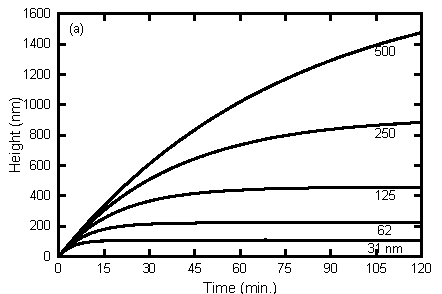
\includegraphics[width=\textwidth]{nanocdte_model_thickness}
  \caption{\label{fig:nanocdte_model_thickness}}
 \end{subfigure}%
 \begin{subfigure}[t]{0.49\textwidth}
  \centering 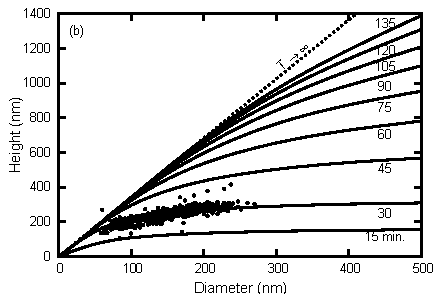
\includegraphics[width=\textwidth]{nanocdte_model_time}
  \caption{\label{fig:nanocdte_model_time}}
 \end{subfigure}
 \caption[Simulated CdTe nanowire dimension distributions]{\label{fig:nanocdte_model}Simulation results showing (a) the time evolution of the nanowire height for the five labelled diameters and (b) time snapshots of the height versus diameter dependence for the times labelled.
  The dashed line shows the linear dependence expected when all nanowires reach an equilibrium condition.
  Superimposed over the simulation is the experimental data (black dots) of \protect{\cref{fig:nanocdte_stats}}.
  The values used in this simulation have been scaled so to fit this experimental distribution.}
\end{figure}

A growth mode driven by direct impingement, where all the adatoms arrive normal to and are incorporated into the nanostructure, will result in a nanowire height distribution that is independent of diameter.
There are, however, other factors that can come into play.
It has been demonstrated both experimentally\cite{Schubert2004a,Wu2002} and theoretically\cite{Kashchiev2006,Chen2006} that the Gibbs-Thomson effect can give rise to a height distribution directly proportional to the nanowire diameter.
The effect stipulates that the higher curvature associated with smaller diameter seeds yields a higher effective vapour pressure, reducing the uptake of atoms from the impinging vapour.
While this effect qualitatively gives rise to the observed CdTe nanowire height distribution, it is unable to account for the observed height limitation for the bismuth seeded nanowires as it provides no means of halting the growth.

The self-limiting growth mode displayed by the bismuth seeded nanowires deposited on an alcohol-altered surface likely originates from an equilibrium that develops between the addition of adatoms through direct impingement on the catalyst and the loss of atoms from the sidewalls through sublimation.
The sublimation process is significant for the CdTe nanowires as they will disappear completely in approximately 30~min if left at the growth temperature without an incoming flux of cadmium and tellurium atoms.
A similar situation must exist for the Bi\textsubscript{2}Te\textsubscript{3} seeded nanowires, but in this case the results are complicated by the distribution of the nanowires' diameters and the lateral growth that becomes apparent for long growth times.
A stochastic simulation was conducted to show the time evolution of the nanowires subject to a sublimation process.
Arrays of nanowires with random diameters were exposed to a simulated random flux of incoming atoms, atoms which caused them to grow larger while surface area caused them to sublimate.
With the uptake of material being proportional to the area of the catalytic seed and the loss of material being proportional to the area of the sidewalls, the simulation yields nanowire heights showing the time evolution presented in \cref{fig:nanocdte_model_thickness}.
Snapshots in time of the nanowire height versus diameter distribution are shown in \cref{fig:nanocdte_model_time} with the experimentally observed distribution of \cref{fig:nanocdte_stats}a superimposed.
The intent of this simulation was not to rigorously model the nanowire growth as it ignores such factors as the Gibbs-Thomson effect.
It does, however, show that sidewall sublimation limits nanowire height and results in a size distribution qualitatively similar to that observed experimentally.

Essential to this work is the observation that Bi\textsubscript{2}Te\textsubscript{3} seeded nanowires show a marked tendency towards lateral growth, while the bismuth seeded nanowires deposited on an alcohol-altered substrate do not.
This tendency is displayed not only at long growth times, but also in the tapering shown at high growth rates and in the elongation of the slanted-top nanowires formed at the edge of the substrates.
These three observations are consistent with the preferential nucleation of adatoms at the base of the nanowire where a weak nucleation site forms due to atomic bonding from both the sidewall facet and the substrate.
Such a nucleation site would be analogous to the ones formed on a vicinal substrate\cite{Ratsch2005a}.
The atoms forming at the base would then have to promote the propagation of a layer up the nanowire's sidewall.
The existence of a lateral growth mode accounts for the formation of tall, large diameter nanowires for extended growth times (\cref{fig:nanocdte_lateral}).
In the initial stages of growth the axial growth rate exceeds the lateral growth rate by a wide margin, but as the nanowire approaches its height limit the axial growth slows dramatically as shown in \cref{fig:nanocdte_model_thickness}.
The model presented, however, does not account for the situation where a slow lateral growth mode accompanies the axial growth.
In this scenario, lateral growth results in larger diameter nanowires which, in turn, allow for increased axial growth.
As a result, both dimensions will grow slowly in tandem provided that the catalytic material remains active as it spreads out over the expanding top surface of the nanowire.

Lateral growth is most evident for the slanted-top nanowires (\cref{fig:nanocdte_lateral}) as it proceeds in an anisotropic manner.
In the PLD process cadmium and tellurium atoms exit the target from an area a few square millimetres in diameter.
Thus, while the ablated material arrives normal to the centre of the substrate, it arrives at an angle to the edges.
As a result, nanowires growing at the edges will have cadmium and tellurium atoms preferentially landing on the sidewall facet nearest to the centre of the substrate.
Thus, the adatoms have an increased likelihood of becoming a part of both the growth front nearest to that sidewall facet as well as any layer propagating up that sidewall.
It is this asymmetry that leads to the anisotropic growth mode that is mirrored on opposite sides of the substrate.

The extent of the lateral growth at the base of the nanowire must be dependent upon the availability of adatoms on the surface of the substrate.
At slow growth rates the nucleation of adatoms will be far more difficult as singly bonded atoms and small clusters of atoms will easily dissociate, making them prone to evaporation from the surface.
At higher growth rates the availability of adatoms increases allowing for larger clusters to stabilize.
Under these conditions the nanowires will have a small, but significant, collection area.
The effect of this collection area, however, will diminish as one moves away from the surface of the substrate, a situation that should give rise to a tapered structure as shown in \cref{fig:nanocdte_tapered}.

As previously mentioned, these lateral growth modes are absent for the bismuth seeded nanowires deposited on an alcohol-altered substrate.
It is our conjecture that during the dewetting process, the bismuth seeds are able to penetrate through this surface-altered layer in a manner that effectively cleans the surface and exposes the (0001) face of sapphire; a face essential to the epitaxial alignment of the nanowires.
This statement is supported by the fact that a bismuth absorption/desorption treatment has been used to remove carbon-containing impurities from the surface of SrTiO\textsubscript{3} and LaAlO\textsubscript{3}\cite{Watanabe1991a}.
Around the periphery of each seed it is expected that the substrate's alcohol surface alteration persists.
As a result, the nucleation site at the base of the nanowire is of poor quality as the substrate's epitaxial relationship no longer exists due to the corrupted surface.
It is this deterioration in the nucleation site that inhibits the nanowire's ability to grow laterally.
In general, poor adhesion of adatoms to the substrate should be detrimental to a lateral growth mode as adatoms must already have a low probability of attaching to the sidewall facet; if this were not the case a one-dimensional nanowire growth mode would be unattainable.
The described process results in lateral overgrowth suppression in a manner analogous to that used for nanowire production through the use of selective area epitaxy.
It is well established that CdTe is prone to such a process as there is a substantive body of work detailing procedures for obtaining selective epitaxy in the CdTe system\cite{Sporken2000,Zhang2001a,Bhat2006a}.
Also supportive of this explanation are reports detailing the fabrication of vertically aligned nanowires, where non-vertically aligned growth is eliminated through the use of organic layers\cite{Krishnamachari2004,Mikkelsen2005,Martensson2007}.

\section{Implications for Symmetry and Energy at Epitaxial Surfaces}
The bond energy landscape of CdTe on oxide substrates like Al\(_2\)O\(_3\) is already not particularly strong, as demonstrated by the CdTe thin film liftoff phenomenon.
The additional chemical fouling of the sapphire substrate with alcohol has had the effect of both reducing the rate of nucleation on the substrate, and the diffusion rate of adatoms on the substrate surface.
The carbon film on the surface is more chemically reactive with the Cd and Te adatoms than they are with the substrate.
Only where the metal seeds are present can the adatoms reach the substrate and begin to assemble into the nanowire.
Such chemical fouling resembles the process of surfactant layers deposited before epitaxial growth to enhance the diffusion of adatoms\cite{PhysRevLett.63.632}.
Here, the layer instead prevents the diffusion of adatoms.

This surface energy modification is a possible route to reducing or eliminating the parasitic thin film present during the growth of semiconductor nanowires.
If the balance of growth temperature and chemical fouling can be optimized, higher quality nanowire devices may be possible.
 
\chapter{III-V Growth on Oxides and Liftoff Phenomenon}
\section{Introduction}

\section{Background}

\section{Experimental}

\section{Results and Discussion}

\section{Implications for Symmetry and Energy at Epitaxial Surfaces}
\part{Noble Metals on Oxides}
\chapter{Nanostructured Gold on Spinel}
\section{Introduction}
As part of the investigations into VLS growth of CdTe nanowires, the control of the size and spatial distribution of metal seeds on oxides was investigated. CdTe nanowire growth had been previously successful using Bi and BiTe seeds, however there are unstable, gold or another noble metal would expand the processing window both in terms of time and temperature. As such, experiments into the control of gold on several oxide substrates was undertaken.

While ultimately nanowire growth was suspendend in favour of other investigations, the research into the interactions of gold overlayers on MgAl\(_2\)O\(_4\) (spinel) substrates yielded some surprising results. The standard method of producing metal seed particles is thermal dewetting, relying upon the relative surface energies of metal versus substrate to cause the film to ball up. The dewetting of gold on spinel substrates was found to result in epitaxial alignment and nanocrystal formation. A full characterization into the formation process of the gold nanocrystals was undertaken and a phenomenological model of their formation was presented.

\section{Experimental}
The gold nanostructures were formed through the deposition of gold films on MgAl\textsubscript{2}O\textsubscript{4} substrates (MTI Corp.)
followed by an annealing procedure which facilitated film
dewetting and nanostructure formation. The films were
sputter-coated at room temperature to a thickness of 5 \AA-15
\AA with a GATAN PECS Model 682 ion beam coating/etching system. The samples were then placed in a tube
furnace with a 100 SCCM flow of argon, heated to 1100 \celsius{}
in 45 min, and then held at that temperature for 1 h.
Following this treatment, the sample was cooled to 1000 \celsius{}
in 30 min, held at that temperature for an additional hour,
and then allowed to cool to room temperature over an interval
of approximately 8 h. Holding the temperature at both 1100
and 1000 \celsius{} was crucial to the formation of the nanostructures described here. Removal of either step results in the formation of faceted gold spheres sitting directly on the substrate.

Scanning electron microscopy (SEM) images of the gold
nanostructures formed on the (100), (111), and (110)
MgAl\textsubscript{2}O\textsubscript{4} substrates, obtained using a JEOL-7000F SEM in
secondary electron mode, are shown in \cref{fig:nanogold_sem}. For each
substrate orientation, one observes two types of features, (i)
spheres supported by a necking region attached to a geometrically shaped base (\cref{fig:nanogold_sem}a-c) and (ii) standalone base
structures (\cref{fig:nanogold_sem}d-f). Convergent beam electron diffraction (CBED) performed using a Phillips CM12 confirmed
that the supported spheres are crystalline. For each case, the shape of the base structure reflects the underlying symmetry
of the substrate which is four-fold, three-fold, and two-fold
symmetric for the (100), (111), and (110) surfaces, respectively. X-ray diffraction measurements, using a Bruker 6000
CCD detector on a Bruker three circle D8 goniometer with
a Rigaku RU-200 rotating anode Cu KR X-ray generator and
parallel-focusing mirror optics, were used to determine the
substrate orientation relative to the edges of the base
structures and are denoted on the three top-down SEM
images (\cref{fig:nanogold_sem}d-f).
\section{Results and Discussion}
The crystallographic alignment of
the nanostructures is a clear indication of epitaxy and
is strongly suggestive of {111} gold faceting of the base
structures associated with the [100]- and [111]-oriented
substrates. For the (110) surface, the standalone base
structures are ill-defined and show no obvious faceting, while
those formed in combination with a sphere show shapes
consistent with mixed faceting, possibly having {111} and
{100} facets for the short and long dimension, respectively.
The standalone base dimensions are remarkably uniform with
side lengths of 40, 65, and 65 nm \(\times\) 110 nm for the (100),
(111), and (110) substrates, respectively.
\begin{figure}
    \centering
    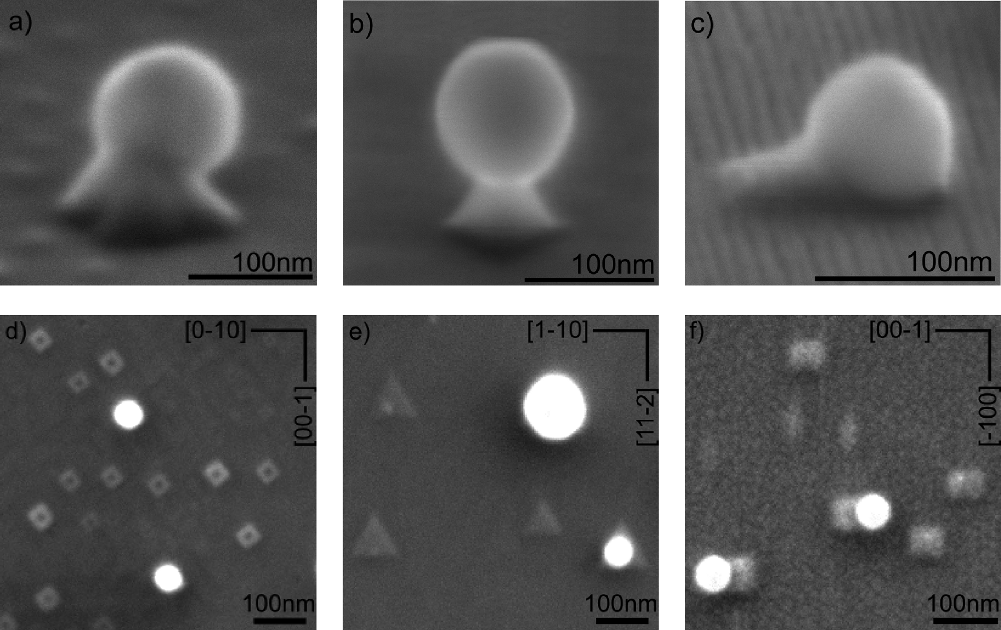
\includegraphics[width=0.8\textwidth]{nanogold_sem}
    \caption[SEM images of gold nanostructures]{\label{fig:nanogold_sem}SEM images showing the gold nanostructures formed
        on MgAl\textsubscript{2}O\textsubscript{4} substrates. The three upper images show spheres
        supported by a necking region attached to a geometrically shaped
        base for the (a) [100]-, (b) [111]-, and (c) [110]-oriented substrates.
        Each of these images was taken at a 70\degree tilt. The aura seen around
        nanostructures is an artifact of imaging. The three lower images
        show the top-down view of both standalone base structures and
        supported spheres for the (d) [100]-, (e) [111]-, and (f) [110]-
        oriented substrates. The in-plane Miller indices of the substrate are
        denoted on each of these images. For all cases, the samples were
        coated with a thin layer of platinum to improve imaging. Imaging
        without platinum shows the same structures but is of poor quality
        due to substrate charging effects.}
\end{figure}

While there are two basic types of nanostructures formed
on each substrate orientation, these structures are found in
various stages of development. For the most part, the bases
are well-developed and show little size variation. The
spherical structures, however, vary dramatically both in their
size and position relative to the base structures. \cref{fig:nanogold_progression} shows a series of top-down SEM images for the case of the
(111) MgAl\textsubscript{2}O\textsubscript{4} substrate showing an evolution of the
nanostructures from a standalone triangular base to bases
supporting spheres of increasing size. Notable is the fact that
the nanostructure, shown in \cref{fig:nanogold_progression}b, manifests itself as a
small sphere which is offset from the centre of the base while for the larger spheres, this asymmetry disappears. Such
asymmetries are observed for all three substrate orientations,
but only those nanostructures formed on the (111) substrate
consistently show a centrally placed sphere for the large
sphere sizes. Also noteworthy is a systematic effect whereby
the size of the triangular base structure increases for sphere
diameters greater than 80 nm (see \cref{fig:nanogold_progression}e and f).
\begin{figure}
    \centering
    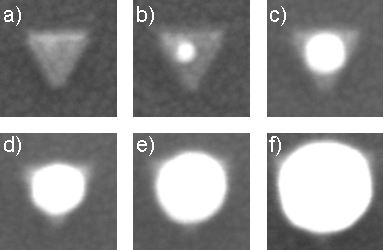
\includegraphics[width=0.9\textwidth]{nanogold_progression}
    \caption[SEM of gold nanostructure growth progression]{\label{fig:nanogold_progression}SEM images showing the top-down view of gold
        nanostructures formed on the (111) surface of MgAl\textsubscript{2}O\textsubscript{4} substrates.
        The sequence of images is chosen to show progressively larger
        spheres atop the base structures. Note that only the smallest sphere,
        shown in (b), is offset from the centre of the triangular base and
        that the base size is slightly larger when supporting larger spheres,
        as is the case for (e) and (f). The size of each image is 130\(\times\)30
        nm\textsuperscript{2}.}
\end{figure}

The base structures formed on each substrate orientation
are a clear consequence of the epitaxial relationship formed
between gold and the latticed-matched MgAl\textsubscript{2}O\textsubscript{4} substrate.
This is apparent from the fact that the geometries of the base
structures mimic the underlying symmetry of the substrates.
It is also likely that the base sizes are a consequence of the
substrate-imposed strains. Arguments based on epitaxy,
however, cannot explain the self-assembly of the gold spheres
atop the base structures and the associated necking behaviour
which facilitates their connection to the base. It is our
hypothesis that the necking behaviour results from an attempt
to minimize the surface energy of the structure. Thus, the
overall shape of these nanostructures is governed by an
interplay between the constraints imposed by epitaxy and a
requirement that the surface free energy be minimized. This
situation has much in common with formation of soap
bubbles affixed to a wire frame\cite{RefWorks:95}. This statement is based
on the facts that the frame imposes a constraint analogous
to that imposed by lattice mismatch and that the shape of
the soap bubble is, to a large degree, determined by the
surface free energy. This analogy provided the impetus for
applying the well-developed models associated with soap
bubble formation to the nanostructures described here. Such
modelling has also been successfully used to predict the
equilibrium shape of biological lipid bilayers (blood cells)
when exposed to abnormal pressure, temperature, magnetic,
and chemical environments\cite{RefWorks:99,RefWorks:102,RefWorks:47,RefWorks:100,RefWorks:101,RefWorks:103}.

The gold nanostructures were modelled as a continuum
elastic surface constrained by a footprint. Three different
footprint geometries (square, equilateral triangle, and rectangle) were used in order to mimic the four-fold, three-fold,
and two-fold symmetries associated with the (100), (111), and (110) surfaces of MgAl\textsubscript{2}O\textsubscript{4}. The size and shape of the
footprint were kept constant during the simulated growths
in order to match the experimental observation indicating a
high degree of base uniformity. For each orientation, the
contact angle (i.e., the angle between the footprint plane and
the tangent plane of any surface connected to the footprint's
edge) was set to a constant where the value was chosen to
be consistent with the observed faceting, as is schematically
shown in \cref{fig:nanogold_facets}.

With these constraints, the shape of an open elastic surface
can be fully described by the mean curvature, H, and the
Gaussian curvature, \(K\), while its corresponding elastic
properties can be characterized by a bending modulus \textkappa and
a Gaussian modulus \textkappa\textsubscript{G}. The surface energy (\(F\)) can then be
formulated as
\begin{equation}
F = \int \frac{\kappa}{2}H^2 dA + \int \kappa_G K dA + \lambda S + PV
\end{equation}
where \textlambda, V, S, and dA are the particle's surface tension,
volume, total surface area, and surface area element, respectively\cite{RefWorks:49,RefWorks:97}. The pressure, P, serves as a Lagrange multiplier
which ensures that a constant volume is enclosed between
the structure and the footprint plane. The second term gives
the integrated Gaussian curvature, which is constant according to the Gauss-Bonnet theorem\cite{RefWorks:98}. For a given surface
tension and volume, the equilibrium shape will correspond
to an energy minimum determined by the shape equation
\textdelta{} F \(=\) 0. The structures are more readily solved by first
rescaling the free energy of the model to become dimensionless, such that
\begin{equation}
\tilde{F} = \int \left (\frac{\tilde{\kappa} \tilde{H}^2}{2} + 1 \right)d \tilde{A} + \tilde{P} \tilde{V}
\end{equation}
where
\begin{align*}
\tilde{A} &= A/S_0 & \tilde{V} &= V/S^{3/2}_0 & \tilde{H} &= H S^{1/2}_0 \\
\tilde{\kappa} &= \kappa / \lambda S_0 & \tilde{P} &= P S^{1/2}_0 / \lambda & \tilde{F} &= F / (\lambda S_0)
\end{align*}
and S0 is the area of the base. Thus, according to this
dimensionless free-energy expression, there are two independent controlling parameters,
\(\tilde{\kappa}\) and \~{P}.

Helfrich and Ou-Yang\cite{RefWorks:49} have analytically solved the shape
equation for some symmetrical geometries. For the work
presented here, the surface is sectioned into discrete elements
using a triangulation mesh, and a simple dissipative model
is used to minimize the energy, as in eq 2\cite{RefWorks:76}
\begin{equation}
    \frac{\delta \mathbf{r}}{\delta t} = - M \frac{\delta \tilde{F}}{\delta \mathbf{r}}
\end{equation}
where \textbf{r}(t) is the position vector of a point on the particle
surface at the time t and M is a kinetic coefficient. These
methods, developed by Taniguchi et al.\cite{RefWorks:76}, are, however,
unable to simulate large deformations. To circumvent this
limitation, we employed two techniques, equiangulation and
vertex averaging, available through the Surface Evolver software developed by K. Brakke.49 Following the procedure of Lim et al.,39,42,43 the curvature was discretized based on
the methods of Julicher,50 which exactly describe the
curvature in the continuum limit. The variational derivative
used in the triangulation scheme was evaluated analytically.
For the Surface Evolver technique, variables were solved
numerically when analytical variations for discrete curvatures
proved difficult.
\begin{figure}
    \centering
    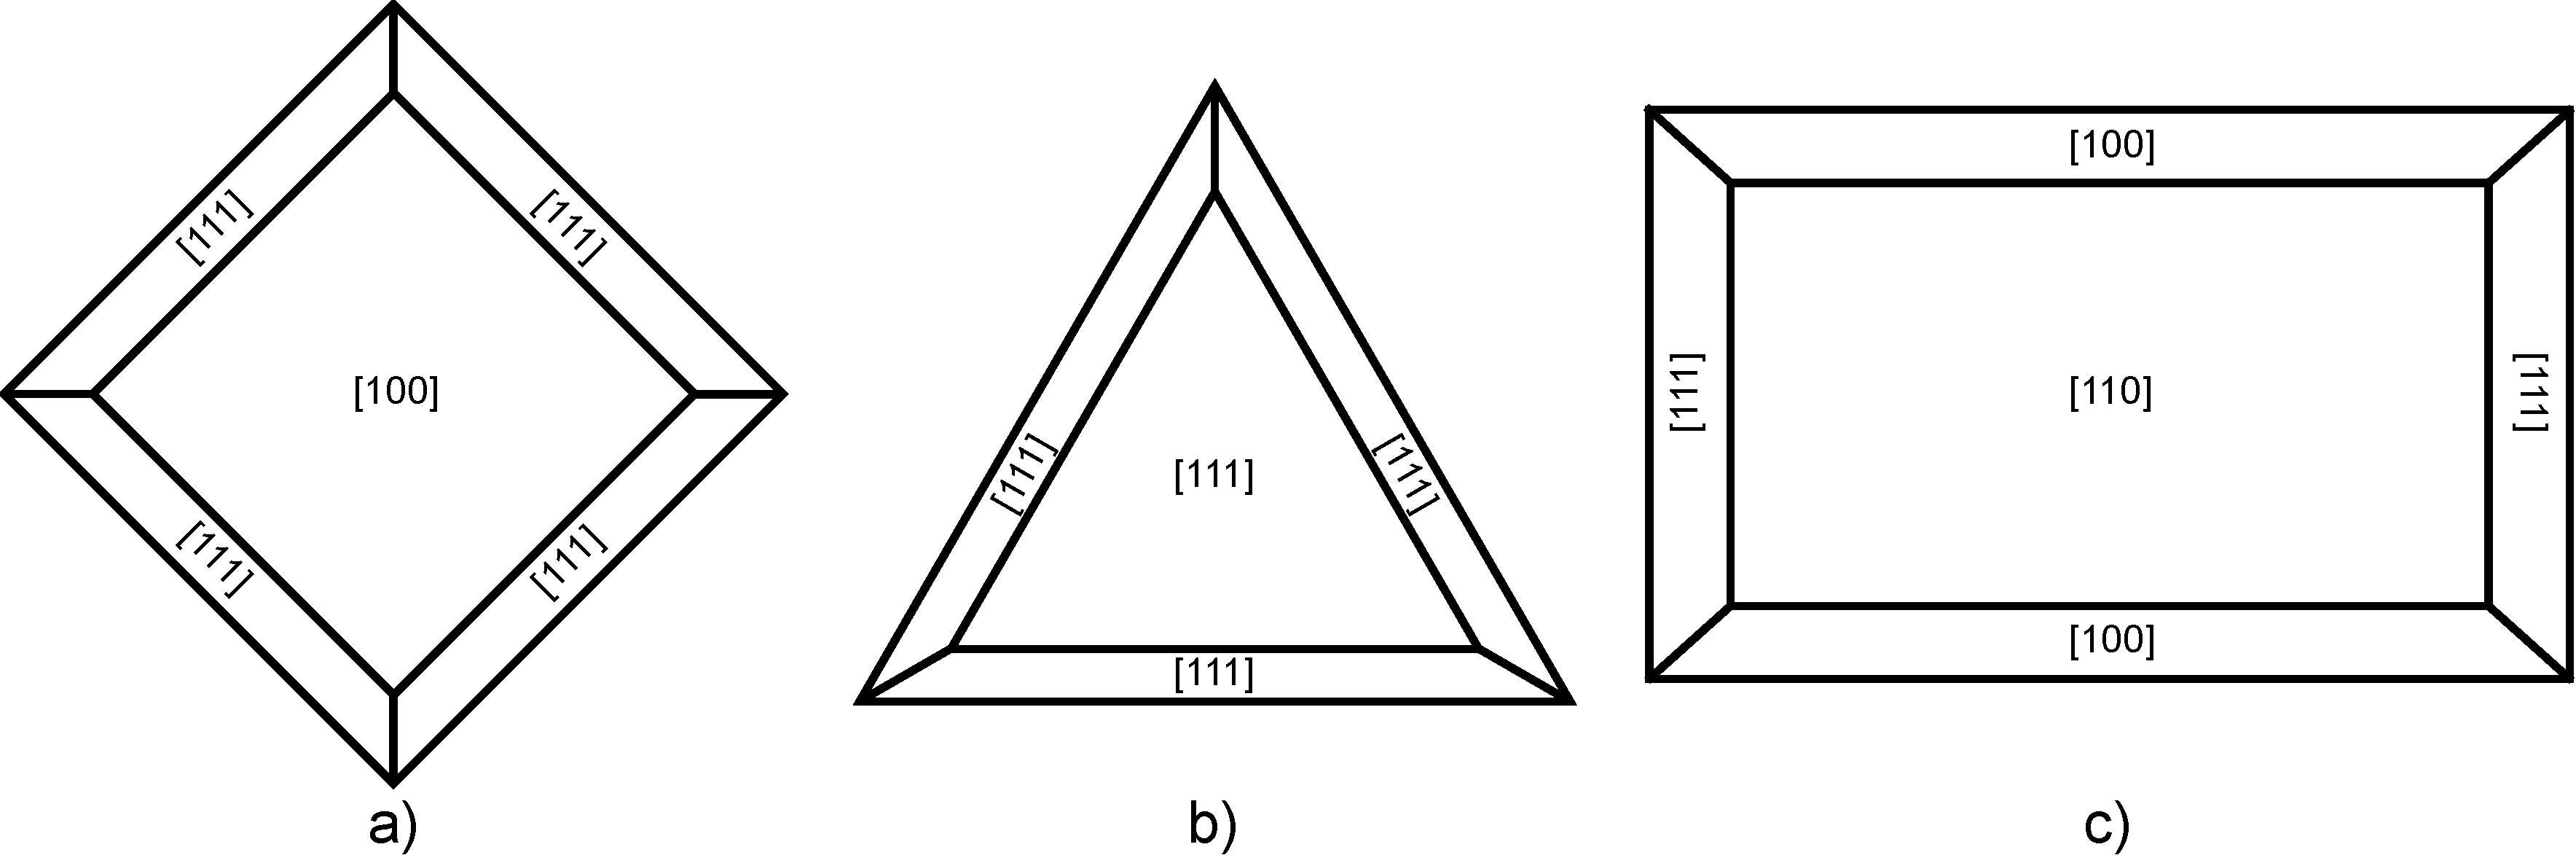
\includegraphics[width=\textwidth]{nanogold_facets}
    \caption[Model of gold nanostructure faceting]{\label{fig:nanogold_facets}Proposed faceting of the base structures grown on (a) [100]-, (b) [111]-, and (c) [110]-oriented substrates.}
\end{figure}
\begin{figure}
    \centering
    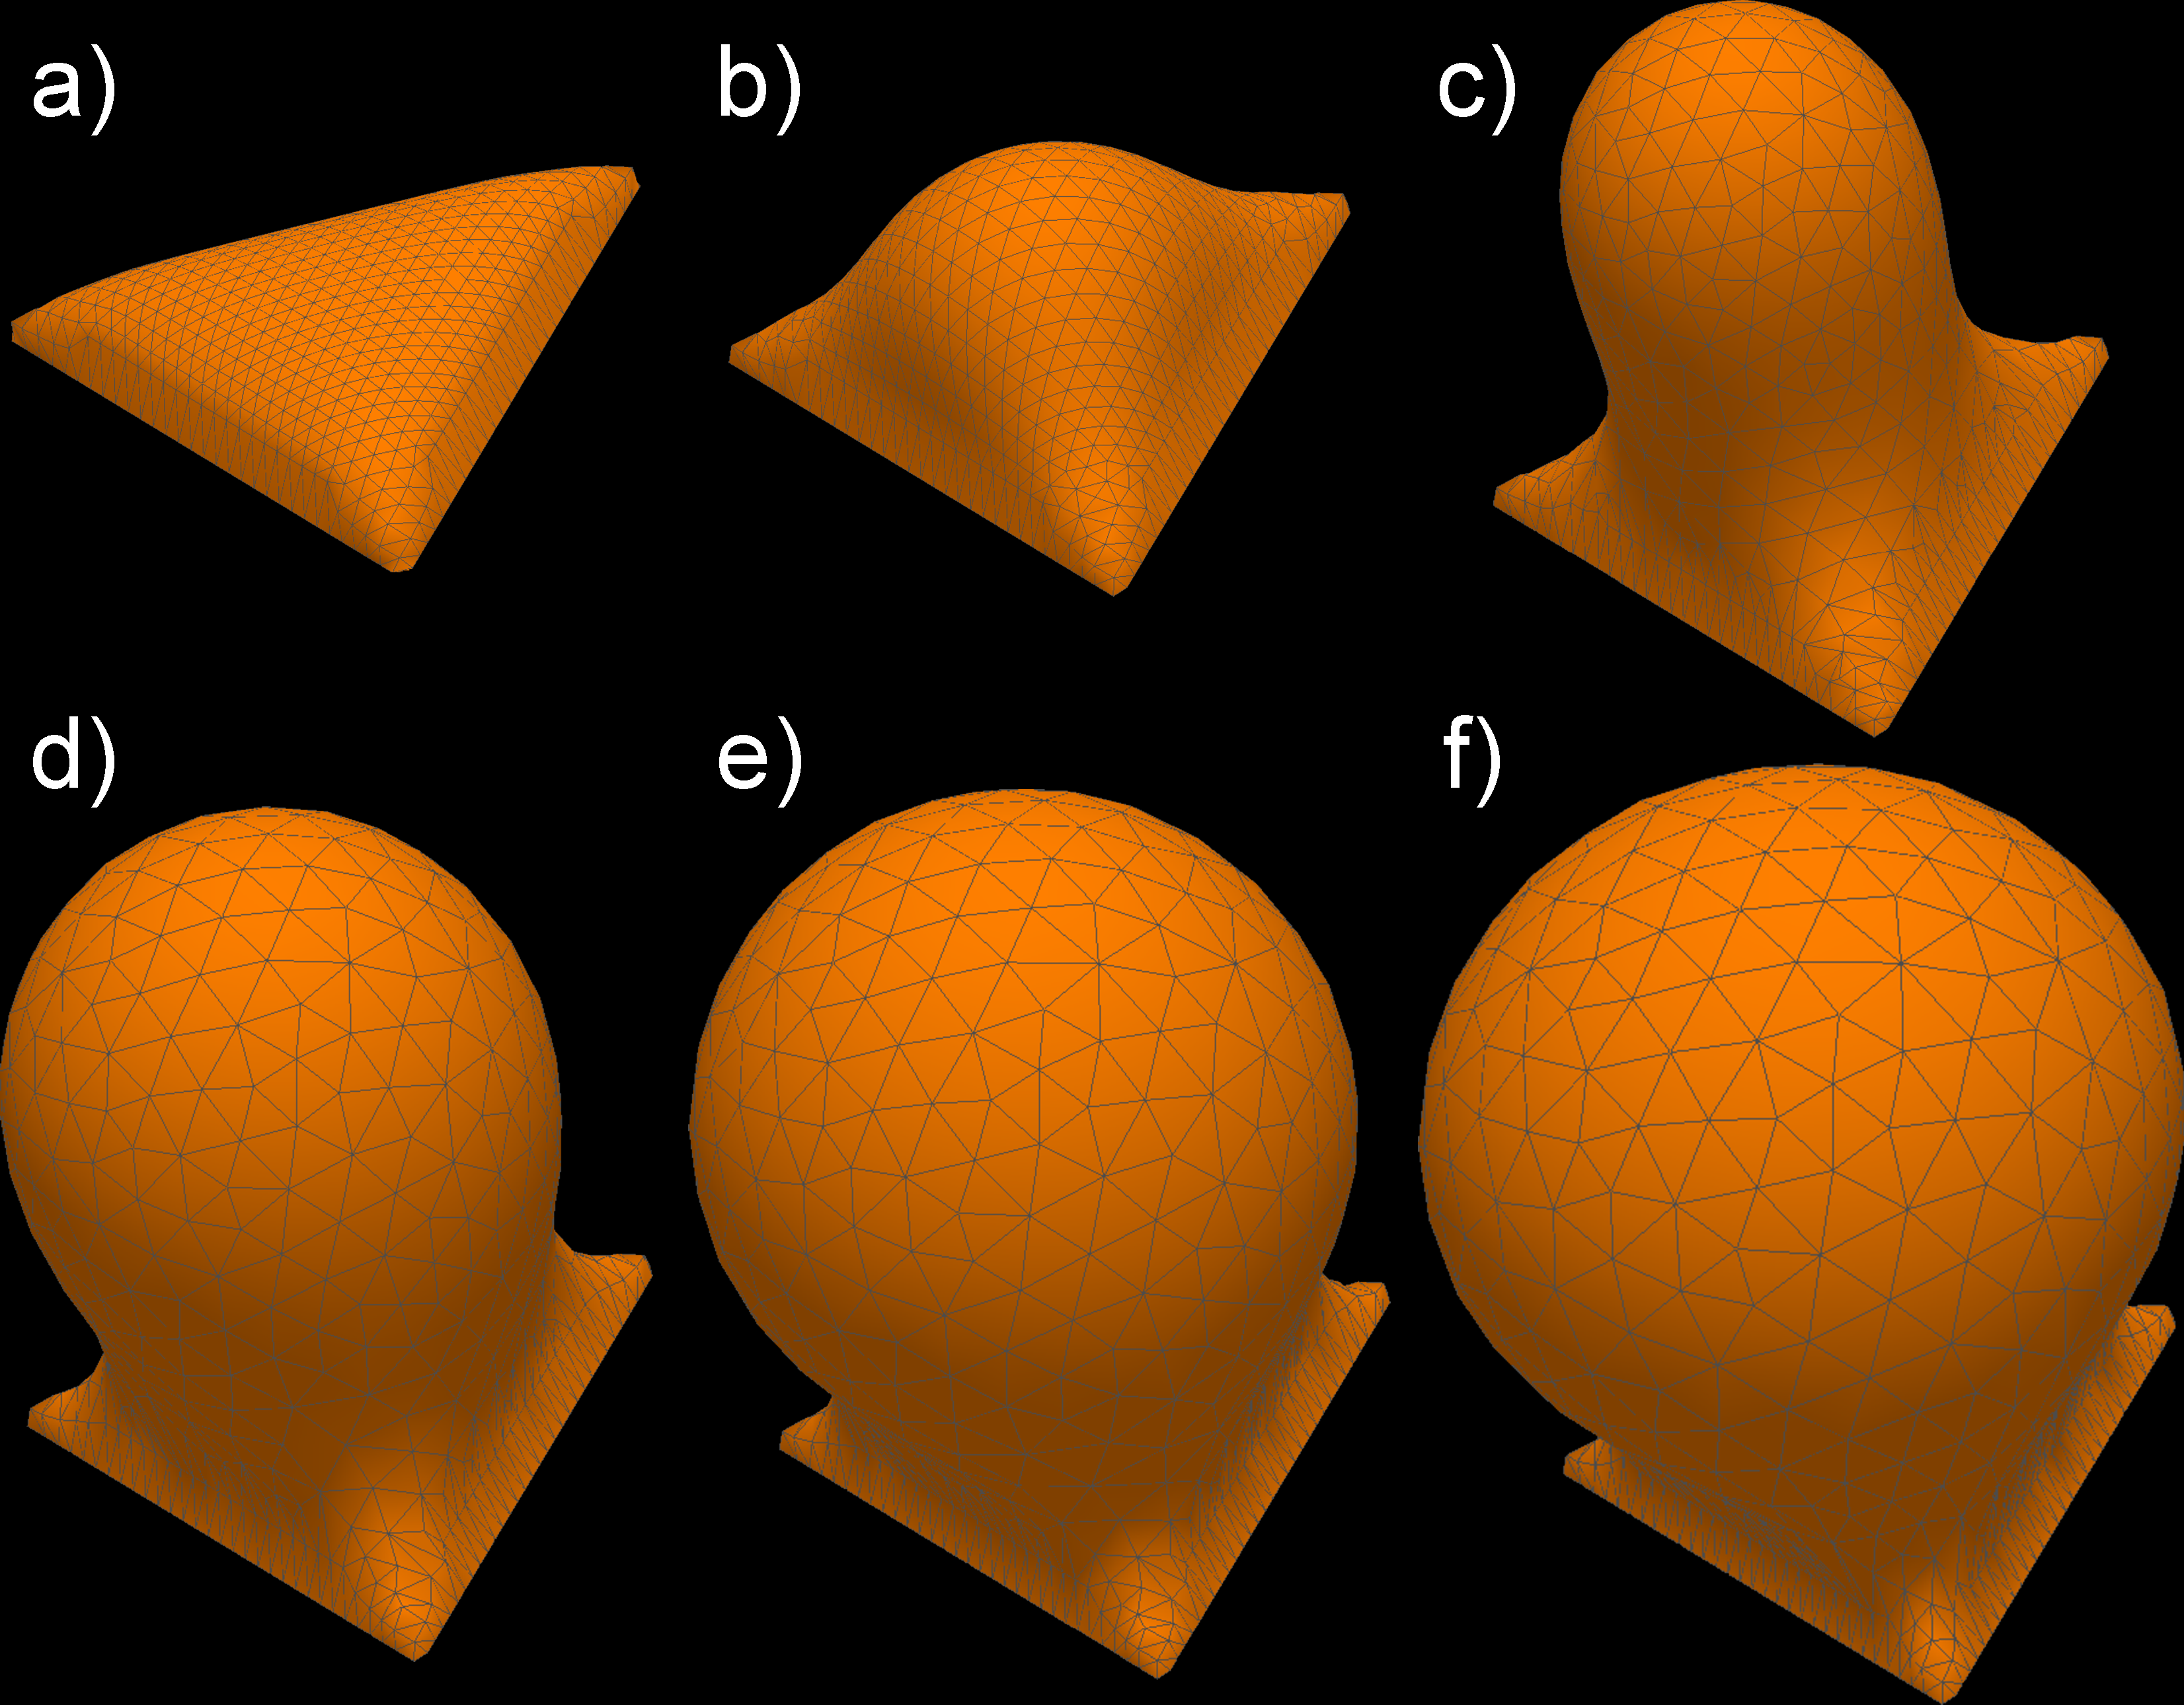
\includegraphics[width=\textwidth]{nanogold_simgrowth}
    \caption[Simulated gold nanostructure growth]{\label{fig:nanogold_simgrowth}Simulations based on the continuum elastic model showing the shape evolution of structures with a triangular footprint as the
        total volume is progressively increased. The shape of these modelled structures is remarkably similar to that of the self-assembled gold
        nanostructures formed on (111) MgAl\textsubscript{2}O\textsubscript{4} substrates (\protect{\cref{fig:nanogold_sem}}b and e and \protect{\cref{fig:nanogold_progression}}). The scale is in arbitrary units.}
\end{figure}

Using the numerical methodology, a progression of
structures with increasing volume were calculated using
square, triangular, and rectangular footprints having contact
angles of 54.7\degree, 70.5\degree, and 35\degree{} (long-axis) by 45\degree{} (short-axis),
respectively. The chosen contact angles are consistent with
the inferred faceting, as shown in \cref{fig:nanogold_facets}. For each case,
the footprint area and surface tension are set to unity, while
the bending modulus is allowed to vary. \cref{fig:nanogold_simgrowth} shows the
calculated progression for the triangular footprint. As the
volume is increased, there is an evolution from a nearly flat
base, to a base with a bulge, and then finally to a spherical
structure supported by a necked region to a triangular base.
These simulated structures are remarkably similar to the gold
nanostructures formed on the (111) MgAl\textsubscript{2}O\textsubscript{4} substrate (see
\cref{fig:nanogold_sem}b and c and \cref{fig:nanogold_progression}). Similar trends are observed for the
square and rectangular footprints. \Cref{fig:nanogold_square_rect} shows the
simulated high volume structures for the square and rectangular footprints, which, once again, are consistent with
experimental observations. The simulations do not, however,
account for any of the observed asymmetries.
\begin{figure}
    \centering
    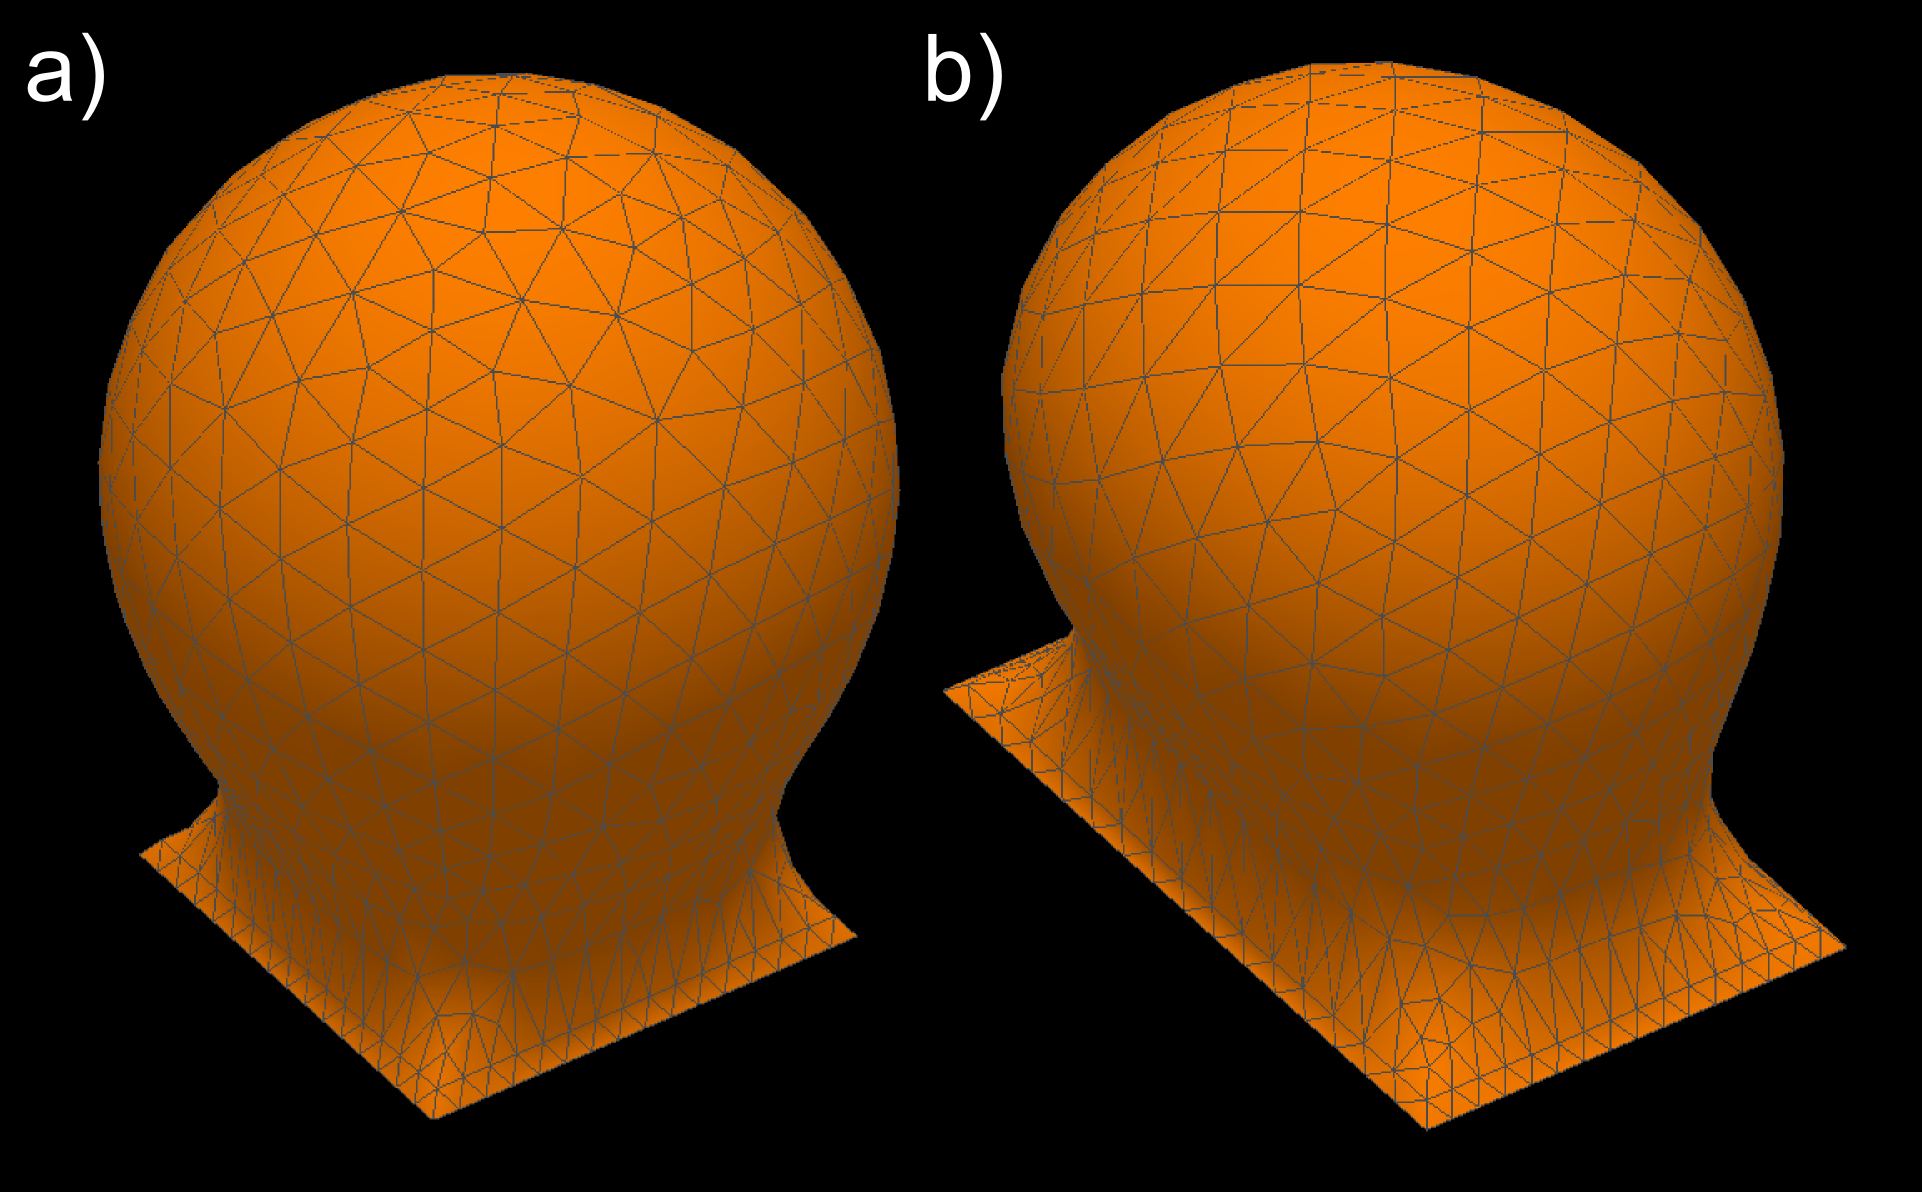
\includegraphics[width=\textwidth]{nanogold_square_rect}
    \caption[Simulations of square and rectangular base gold nanostructures]{\label{fig:nanogold_square_rect}Simulations based on the continuum elastic model
        showing the expected high volume shape for the (a) square and
        (b) rectangular (length/width ) 1.42:1) footprints. These structures
        show a resemblance to the self-assembled gold nanostructures
        formed on the (100) and (110) MgAl\textsubscript{2}O\textsubscript{4} substrates (\protect{\cref{fig:nanogold_sem}}) but
        show none of the observed asymmetries. The scale is in arbitrary
        units.}
\end{figure}

The shape of the base structures of the self-assembled gold
nanostructures is strongly influenced by epitaxy and the underlying symmetry of the substrate surface. That being
said, it is difficult to account for the hollowed-out center
observed for the base structure formed on the (100) MgAl\textsubscript{2}O\textsubscript{4}
using epitaxy-based arguments. This feature is, however,
predicted by the continuum elastic model. \Cref{fig:nanogold_afm}a shows
the topographical color map obtained from the modelling for
the low-volume structure. It clearly shows a circular depression in the middle of the structure as well as a lobe near
each corner. Motivated by the simulation results, we
examined the topography of the self-assembled gold nanostructure using atomic force microscopy (AFM). \Cref{fig:nanogold_afm}b
shows a tapping mode AFM image of the base structure
obtained using a Digital Instruments scanning probe microscope (SPM) and a NanoScope IIIa controller. Even though
the features of the nanostructure are somewhat washed out
due to the fact that the resulting image is a convolution of
the nanostructure and the AFM tip geometry, the nanostructure's four lobes and central depression are clearly visible.
\begin{figure}
    \centering
    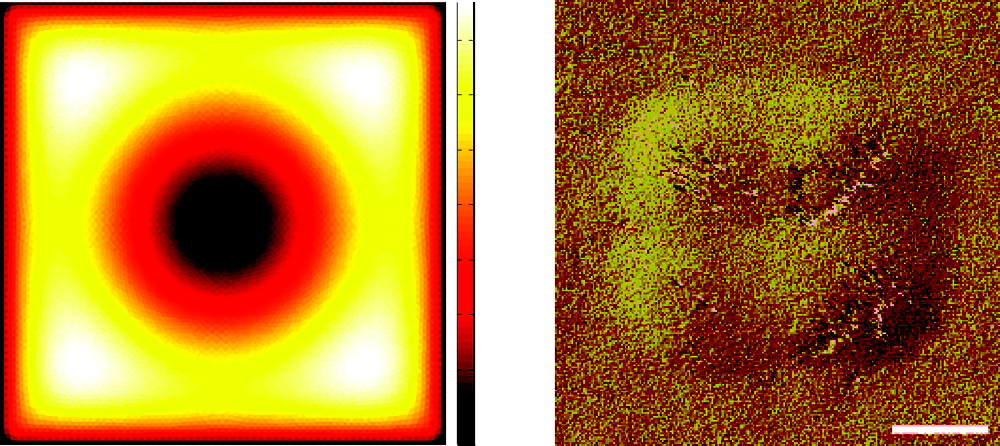
\includegraphics[width=0.8\textwidth]{nanogold_afm}
    \caption[Comparison of AFM and simulated gold nanostructure topography]{\label{fig:nanogold_afm}A comparison of the (a) topographical colour map derived
        from the continuum elastic model and (b) the AFM image of a
        self-assembled gold nanostructure deposited on the (100) MgAl\textsubscript{2}O\textsubscript{4}
        substrate. Note that the simulation predicts both the presence of
        four lobes at the corners and a central depression. The scale of the
        topographic image is arbitrary, and the scale of the AFM image is
        10 nm.}
\end{figure}

Taken together, the experimental observations and the
continuum elastic modelling results strongly suggest that
epitaxy and a minimization of the surface free energy are
the two primary drivers in determining the shape and size
of the self-assembled gold nanostructures. The fact that
similar structures have not been previously observed is likely
a consequence of the synthesis route used. The route employed here not only involves temperatures well in excess
of those typically used when forming substrate-supported
nanostructures but also requires an annealing profile which
accesses two temperatures. It is possible that the initial 1100 \celsius~anneal is needed to induce surface reconstructions in the
MgAl\textsubscript{2}O\textsubscript{4} substrates which are essential to the growth of these
nanostructures. Surface reconstructions have been shown to
strongly influence the growth of both nanostructures\cite{RefWorks:24,RefWorks:16,RefWorks:104}
and thin films\cite{Neretina2009a} when using (100) SrTiO3 substrates. We,
however, consider it more likely that the formation of these
nanostructures requires temperatures in excess of the melting
point of bulk gold (1064 \celsius). Significant deviations from
the bulk value, due to finite size effects, are considered
unlikely since such effects appear to occur only in nanostructures smaller than 5 nm\cite{RefWorks:43}. Once molten, the nanostructures are cooled to 1000 \celsius~and held at this temperature,
which is just below the melting point. Such a temperature
allows for solidification while maintaining high adatom
mobility. The fact that this fabrication step is crucial to the
formation of the observed intricate nanostructures provides
compelling evidence that considerable adatom motion is
essential. In this scenario, it is likely that an Ostwald-like
ripening process will play a role where larger nanostructures
grow at the expense of smaller ones. Substrate surface steps,
due to the inherent miscut of the substrate\cite{RefWorks:69}, could also
influence the process by providing energetically favorable
nucleation sites. Nanostructure formation is also heavily
reliant on the epitaxial relationship between the nanostructure
base and the underlying substrate. This relationship determines the crystallographic alignment of the base structures,
while the consistency in size is likely a consequence of the
strain imposed by lattice mismatch. Once the 1000 \celsius~anneal
ends, the adatom motion will be quickly quenched by the
lower temperatures, allowing no further alterations to the
shape or size of the nanostructures. The end result is
intricately shaped nanostructures whose size and shape are
determined by a minimization of the surface free energy
while simultaneously being subject to the constraints imposed
by epitaxy.
\section{Implications for Symmetry and Energy at Epitaxial Surfaces}
Despite the materials of interest in this investigation consisting of a noble metal and a complex oxide, materials which one would not expect any kind of interaction, result in epitaxial alignment. This epitaxial alignment is simple in the sense that the nanocrystal orientations follow directly from the underlying substrate. The epitaxial alignment is complicated by the fact that gold fits onto  sublattice of half of a MgAl\textsubscript{2}O\textsubscript{4} lattice. Such epitaxy relies on the symmetry of the surface atoms forming a lattice with a smaller lattice constant than the bulk crystal. This epitaxy can thus be thought of as nanocrystal forming on a reconstructed surface, since the surface atoms present a surface net with a different lattice parameter than the bulk.

The more surprising result from this work is the epitaxial alignment possible between very nonreactive materials. Noble metals are not known to readily react with other elements or compounds other than to form simple metallic bonds. Similarly, metals in general are not known to strongly wet oxide surfaces, preferring to bond to themselves instead. Complex oxides are also known to be very stable to high temperatures, and stable to a great many compounds. To mix such two compounds and observe something other than segregation and no interaction is surprising. These experiments have shown that, despite there being a very weak interaction between the two materials, due to low reactivity, epitaxial alignment is achieved through a careful thermal treatment. The subtle influence of the substrate's lattice can impart alignment of the gold, overriding the tendency to form a equilibrium crystal shape.


\printbibliography
%\printindex
\end{document}
